\documentclass[a4paper,11pt]{report}
\usepackage[a4paper, margin=3cm, bottom=2.5cm]{geometry}
\usepackage{setspace}
\usepackage{amssymb, amsfonts, amsmath, latexsym}
\usepackage{graphicx, color}
\usepackage{booktabs}
\usepackage{array}
\usepackage{hyperref}

\graphicspath{{figures/evaluation/}}
\pagestyle{plain}

\newtheorem{theorem}{THEOREM}
\newtheorem{lemma}[theorem]{LEMMA}
\newtheorem{corollary}[theorem]{COROLLARY}
\newtheorem{proposition}[theorem]{PROPOSITION}
\newtheorem{remark}[theorem]{REMARK}
\newtheorem{definition}[theorem]{DEFINITION}
\newtheorem{fact}[theorem]{FACT}
\newtheorem{problem}[theorem]{PROBLEM}
\newtheorem{exercise}[theorem]{EXERCISE}

\def \set#1{\{#1\} }

\newenvironment{proof}{
PROOF:
\begin{quotation}}{
$\Box$ \end{quotation}}

\newcommand{\nats}{\mbox{\( \mathbb N \)}}
\newcommand{\rat}{\mbox{\(\mathbb Q\)}}
\newcommand{\rats}{\mbox{\(\mathbb Q\)}}
\newcommand{\reals}{\mbox{\(\mathbb R\)}}
\newcommand{\ints}{\mbox{\(\mathbb Z\)}}

\title{Know Your Limits: Delay-Based Passive Estimation of Remaining Path Capacity}
\date{18 May 2026}
\author{Savani Sawaikar\\
Master of Engineering Computer Science\\
Supervised by Dr. Stefano Vissicchio}

\begin{document}

\onehalfspacing
\pagenumbering{gobble}

\begin{titlepage}
\centering
\vspace*{2cm}
{\Large\bfseries Know Your Limits: Delay-Based Passive Estimation of Remaining Path Capacity\par}
\vspace{1.5cm}
{\large SBBP4\par}
\vspace{0.5cm}
{Master of Engineering Computer Science\par}
{University College London\par}
\vspace{0.5cm}
{Supervised by Dr. Stefano Vissicchio\par}
\vspace{0.5cm}
{18 May 2026\par}
\vfill
\begin{minipage}{0.9\textwidth}
\small
This report is submitted as part requirement for the MEng Degree in Computer Science at UCL. It is substantially the result of my own work except where explicitly indicated in the text.

The report may be freely copied and distributed provided the source is explicitly acknowledged.
\end{minipage}
\end{titlepage}

\begin{abstract}
Network operators must infer remaining path capacity from incomplete measurements, while avoiding measurement traffic that perturbs the path being measured. This project studies whether the packet-delay distribution observed at the receiver can provide a useful passive signal for this problem. Rather than reducing delay to a mean, percentile, or scalar counter, the monitor reconstructs an empirical delay distribution, applies adaptive stopping to decide when that reconstruction is stable, and then compares stopped distributions as offered load changes.

The statistical evaluation connects reconstruction to finite-domain distribution learning and uses total variation distance to measure how quickly discrete and continuous delay distributions can be learnt. The tested distributions converge well before the worst-case theoretical sample bound. For the continuous normal, lognormal, and Weibull cases, kernel density estimation reaches the 0.05 total variation distance target at 500 samples.

The online evaluation replaces access to ground truth with adaptive stopping. Consecutive cumulative reconstructions are compared after packet batches, and the experiments identify \(B=200\) and \(\theta=\delta/6\) as a reliable continuous operating point across the three tested delay families. This setting is treated as an empirical operating choice, not as a theoretical guarantee.

The capacity use case is evaluated in Network Simulator 3 under constant-rate cross traffic, Pareto on-off bursty traffic, and a heterogeneous slow-link stress test. The initial hypothesis that first distributional change marks capacity is rejected because it fires too early. A stronger criterion based on the rate of change of total variation distance detects a capacity-relevant boundary at the 0.925 load-grid point in both single-link and two-to-ten-hop constant-rate experiments. Under bursty traffic, the detected average-load boundary moves to 0.475 because the on-period traffic rate is twice the swept average. In the heterogeneous five-hop test, the same 0.925 grid point is recovered when the slow link is first, middle, or final. A final constructed multi-path modal experiment shows that, in the tested separable mixture, the capacity response should be associated with the changing mode rather than the whole mixture. The work does not provide an exact physical capacity measurement. It shows that passive distributional monitoring can expose when a path leaves its previous low-load operating regime.


\end{abstract}

\clearpage
\pagenumbering{arabic}
\setcounter{page}{1}
\tableofcontents

\chapter{Introduction}

Network operators must infer path headroom from measurements that are often intrusive, incomplete, or too coarse to explain why performance has changed. Modern services run over networks whose traffic mix, topology, routing state, queue occupancy, and failure modes change continuously. A central version of this problem is remaining path capacity, meaning how much additional traffic a path can absorb before delay or user-visible performance starts to degrade. Overestimating this headroom risks congestion and service disruption. Underestimating it wastes capacity and can lead to unnecessary routing or provisioning decisions.

Delay is one of the most accessible signals for this question, but it is often compressed too early. Operational systems commonly report mean round-trip time, high-percentile latency, link utilisation, or threshold alarms. These summaries are useful, but each is a scalar view of a richer object. A path whose mean delay remains stable may still be developing a heavier tail. A second delay mode may appear when traffic is rerouted through a longer path or when queues begin to form intermittently. Two path states can have similar percentile values while having different distributional shapes and therefore different operational implications. Treating delay as a distribution rather than as a single number keeps this information available.

The central question is whether receiver-visible delay samples contain enough information to detect when a path leaves its low-load delay regime. The intended monitor observes packet delays, reconstructs the empirical delay distribution, decides when that reconstruction is stable, and then uses distributional change to infer whether increasing offered load has pushed the path into a different regime. The configured capacity of a simulated link may be used after an experiment to assess error, but it is not available to the monitoring algorithm. The method is designed to reason from observations, not from knowledge of the network configuration.

Existing monitoring systems tend to fall into three groups: active tools that infer available bandwidth by injecting load, telemetry systems that expose queue or hop state from inside the network, and threshold systems that detect anomalies through scalar summaries. The gap addressed here is narrower. The question is whether receiver-visible delay distributions alone can identify the point at which a path leaves its low-load operating regime, and whether that decision can be made without ground-truth capacity or queue state.

\section{Aims and contributions}

The aim of the project is to test whether delay distributions can be treated as a practical monitoring object for estimating a capacity-relevant boundary. This is narrower than general anomaly detection and weaker than direct queue telemetry, but it is chosen because it only assumes receiver-visible delay samples. A successful result would show that distributional monitoring can provide useful evidence before a coarse endpoint alarm is triggered, without requiring the monitor to know the underlying delay family or the true link capacity.

The work is organised around four sub-goals. The first is to establish the statistical basis for learning an unknown delay distribution from samples. The second is to decide when such a reconstruction is stable enough to be used online, where ground truth is unavailable. The third is to turn the stopped reconstruction into an identity decision between operating states. The fourth is to test whether that decision remains meaningful as the network setting moves from direct sampling to a single link, longer paths, and separable multi-path mixtures.

These goals are expressed as three research questions in Table \ref{tab:research-questions}. They are intentionally sequential. A capacity-boundary decision made from delay distributions is only meaningful if the distribution can first be reconstructed, if the reconstruction can be stopped without access to truth, and if the resulting comparison identifies more than ordinary low-load drift.

\begin{table}[htbp]
\centering
\small
\begin{tabular}{p{0.12\textwidth}p{0.78\textwidth}}
\toprule
Question & Focus \\
\midrule
RQ1 & Can an unknown delay distribution be reconstructed from receiver-side samples within a total variation distance target of \(\delta=0.05\)? \\
RQ2 & Can stability between consecutive reconstructions act as an online stopping signal when the true distribution is unavailable? \\
RQ3 & Can changes in stopped delay distributions identify a capacity-relevant boundary as offered load increases, including when the path becomes longer or the receiver sees a mixture of path behaviours? \\
\bottomrule
\end{tabular}
\caption{Research questions addressed by the evaluation.}
\label{tab:research-questions}
\end{table}

The chapter order follows this development. The use case first defines the monitoring pipeline and the intended capacity decision. The statistical chapter then tests whether an unknown delay distribution can be reconstructed from samples. Adaptive stopping tests whether that reconstruction can be trusted without seeing ground truth. The network chapters then use the same stopped distributions to refine the operational decision rule across single-link, multi-hop, and multi-path settings.

The claim is bounded. The report does not claim to measure exact physical capacity. The output is a distributional boundary: the first offered-load region where the observed delay distribution begins moving away from the low-load state much faster than its previous trend. Configured link capacity is used only for post-hoc evaluation in simulation.

The contributions are summarised in Table \ref{tab:intro-contributions}. The main research result is the replacement of first distributional change with a response-rate criterion. Capacity pressure is better identified by the point where total variation distance begins increasing much faster than its previous low-load trend, rather than by the first point where two empirical distributions differ.

\begin{table}[htbp]
\centering
\small
\begin{tabular}{p{0.12\textwidth}p{0.78\textwidth}}
\toprule
Contribution & Summary \\
\midrule
C1 & An empirical calibration of non-parametric delay-distribution reconstruction against a finite-domain total variation distance learning reference. \\
C2 & An adaptive stopping evaluation that shows where consecutive-estimate stability is reliable, and where false stability causes premature stopping. \\
C3 & A capacity-boundary evaluation showing that first distributional change is too sensitive, while a response-rate criterion gives a repeatable boundary under constant-rate single-link and multi-hop conditions and remains interpretable under bursty and heterogeneous stress tests. \\
C4 & A constructed multi-path modal analysis showing that separable receiver-side mixture distributions should be decomposed before capacity association, because whole-mixture TVD can dilute or misplace the stressed path response. \\
\bottomrule
\end{tabular}
\caption{Main contributions of the work.}
\label{tab:intro-contributions}
\end{table}

\section{Network performance context}

The difficulty of this task begins with the structure of the networks being monitored. Large data-centre networks are designed to provide high bisection bandwidth, path diversity, and efficient resource pooling. Fat-tree and Clos-derived designs made it possible to construct large fabrics from commodity switching elements, while systems such as VL2 and Jupiter demonstrate how multi-stage topologies and centralised control can support large-scale cloud services \cite{alFaresFatTree,greenbergVl2,singhJupiter}. These designs improve aggregate capacity, but they also create a measurement problem. Traffic can traverse multiple equal-cost paths, failures can be masked by rerouting, and a performance problem may be visible only as a change in latency, queueing, or flow completion time.

The transport layer adds another reason to care about delay distributions. Data Center TCP (DCTCP), a variant of Transmission Control Protocol, was motivated by the coexistence of latency-sensitive short flows and throughput-hungry background flows, where queue build-up from large flows can harm foreground latency even before severe congestion dominates \cite{alizadehDctcp}. This setting shows why a scalar utilisation counter can be misleading. A link may not appear fully saturated on average, while packet delay begins to show a longer tail or a second operating mode. Remaining capacity is therefore not only a question of nominal link rate. It is a question about when the path's observed behaviour leaves the regime in which it can support additional traffic without unacceptable delay.

Traditional network-management mechanisms provide the historical baseline. Simple Network Management Protocol (SNMP) defines a manager-agent architecture for reading and controlling management information on network devices \cite{harringtonSnmp}. Flow-level systems such as NetFlow export records describing unidirectional Internet Protocol flows, while sampled flow (sFlow) uses packet and counter sampling to support continuous traffic monitoring in high-speed switched and routed networks \cite{claiseNetflow,phaalSflow}. These mechanisms are valuable because they scale to large deployments and have become part of operational practice. Their limitation for this project is their abstraction. Interface counters and flow records are well suited to accounting, capacity planning, and coarse anomaly detection, but they do not directly provide a stable empirical distribution of packet delay on a path.

The key design tension is therefore granularity against overhead. Fine-grained monitoring reveals short-lived queueing and path behaviour that coarse counters miss. However, observing every packet, carrying per-hop metadata, or injecting synthetic probe traffic can consume bandwidth, switch resources, or operational effort. The approach studied here occupies the low-assumption side of that trade-off. It treats delay samples visible at the measurement edge as the primary evidence, then asks how much can be inferred statistically before requiring richer network instrumentation.

\section{Active monitoring}

Active measurement estimates path properties by sending measurement traffic. This family is important because the capacity use case is naturally tempting to frame as active probing. Pathload estimates available bandwidth by sending self-loading periodic streams and detecting increasing one-way delay trends when the probing rate exceeds the available bandwidth \cite{jainDovrolisPathload}. PathChirp improves efficiency by sending exponentially spaced probe trains, extracting information from the rate range covered by each chirp rather than repeatedly probing at a single rate \cite{ribeiroPathchirp}. Packet-pair and packet-train dispersion methods infer capacity or available bandwidth from the spacing of probe packets after they traverse a bottleneck, while Spruce was proposed as a lightweight alternative evaluated against Pathload and Initial Gap Increasing or Packet Transmission Rate methods over wide-area paths \cite{dovrolisPacketDispersion,straussSpruce}.

These methods provide a clear conceptual foundation because delay trends and packet spacing contain information about spare capacity. They are also attractive because they can be deployed from end hosts without requiring internal switch support. The difficulty is that the measurement traffic is part of the experiment. A probe stream must be large enough to reveal congestion, but that same stream can perturb the path being measured. The problem is more acute when the operational question is how much headroom remains. Near the boundary, extra traffic is not merely a measurement cost; it is the mechanism that may push the path into a worse regime.

Coverage-oriented active systems make a different trade-off. Pingmesh continuously measures latency between servers at large scale, while RD-Probe combines randomised and deterministic probing to cover physical components in complex data-centre networks \cite{guoPingmesh,dingRdProbe}. These systems are valuable because they show how active measurement can make hidden network states visible across a large deployment. Their objective, however, is coverage and troubleshooting rather than learning a full delay distribution at a capacity boundary.

Active tools also usually compress their output into a rate estimate or a reachability result. That is appropriate when the goal is to report available bandwidth or path coverage, but it discards some of the signal that appears before, during, and after the rate boundary. A path approaching congestion may first show changes in skew, tail mass, or multimodality rather than a single monotonic delay trend. The capacity use case in this report still changes offered load experimentally, because the goal is to validate whether a capacity boundary can be detected. The monitoring decision, however, is made from the empirical delay distributions observed at each operating point rather than from a direct probe-rate equation. The eventual measurement object is the distributional state of the path under the current load, rather than the probe stream itself.

\section{Passive monitoring}

Passive monitoring avoids injecting dedicated measurement traffic and instead uses traffic already visible to the monitor. For the remaining-capacity use case, this is the more natural target interface. If a monitor can infer a capacity-relevant change from observed delays, then it can run continuously without consuming the headroom it is trying to estimate. Passive monitoring also aligns with operational settings where active probes are undesirable because of policy restrictions, customer traffic sensitivity, or the risk of perturbing short-lived congestion events.

Large-scale passive and hybrid systems show the breadth of this design space. Fathom passively samples remote procedure calls in Google's production fleet and decomposes application latency into client, network, and server components \cite{qureshiFathom}. It is powerful because it links network performance to application-level work and aggregates sampled measurements into distributions. Its measurement interface is nevertheless service-specific and relies on host and stack instrumentation. PIRATE addresses a different visibility constraint by estimating response latency when only one traffic direction is visible under asymmetric routing, using causal request pairs and packet timing gaps \cite{shobhanaPirate}. This demonstrates that packet timing can reveal latency information even when visibility is incomplete. The inferred quantity, however, is response latency from causal structure rather than a path delay distribution used to estimate capacity headroom.

Other systems use passive packet capture or packet histories to improve diagnosis. NetSight records packet histories so that operators can query how packets moved through a network, while Everflow traces selected packets in large data-centre networks using match-and-mirror functionality and analysis servers \cite{handigolNetSight,zhuEverflow}. These systems offer packet-level diagnostic power, but the price is a heavier measurement substrate. They need packet capture, mirroring, collection infrastructure, or packet histories. For debugging and root-cause analysis that cost can be justified. It is still a different operating point from a lightweight edge monitor that estimates whether the delay distribution of a path has changed.

Fine-grained passive systems also show why sub-second and microsecond effects cannot be ignored. Trumpet uses end-host triggers to detect network-wide events at millisecond timescales while inspecting packets at line rate \cite{moshrefTrumpet}. \(\mu\)Mon compresses microsecond-level flow-rate curves using wavelets and replays congestion events to recover short-lived dynamics \cite{zhengMuMon}. These systems reinforce the motivation for moving beyond slow counters. They also highlight a distinction in scope. Their primary objects are events, triggers, or rate curves. The object here is a learned delay distribution, and the central question is whether its stable shape changes as load approaches a capacity limit.

\section{Programmable and in-band telemetry}

Programmable data planes and in-band network telemetry (INT) provide the strongest visibility when the infrastructure supports them. The P4 INT specification allows packets to carry switch-local metadata such as hop latency, queue occupancy, timestamps, and egress utilisation as they traverse the network \cite{p4IntSpec}. Marple proposes a performance query language and switch hardware primitive for line-rate aggregations such as moving averages over queueing latency per flow \cite{narayanaMarple}. ConQuest uses programmable-switch data structures to identify flows that contribute significantly to queue build-up, reporting high precision at millisecond timescales with a small memory footprint \cite{chenConQuest}. UnivMon provides a more general sketch-based framework for estimating network-wide monitoring metrics such as heavy hitters and entropy using programmable measurement \cite{liuUnivMon}.

These systems are compelling because they observe the network close to where queueing occurs. If a switch can report queue occupancy, hop latency, and per-flow contributions, then capacity-related diagnosis can be much more direct. The disadvantage is that this assumes cooperation from the network core. The monitor needs programmable devices, switch resources, telemetry headers, mirrored traffic, or collection infrastructure. That assumption is not always available. It is particularly restrictive for a method intended to reason from path observations rather than from device-local state.

In-band network telemetry also has an overhead problem. Carrying hop-by-hop metadata in packets increases packet size and can affect application performance. Probabilistic in-band network telemetry (PINT) responds to this by encoding telemetry information across packets so that per-packet overhead can be bounded, even as low as one bit for some queries \cite{benBasatPint}. The existence of PINT is itself evidence that raw INT is not free. Reducing overhead is possible, but it introduces a telemetry design problem involving what information should be encoded, how accurately it should be recovered, and which packets should carry it.

The approach in this report is weaker in instrumentation but stronger in deployability. It does not claim to replace INT when switch-local queue state is available. Instead, it targets the complementary case where such support is absent or too expensive. The comparison is therefore not that passive distributional monitoring reveals more than programmable telemetry in an instrumented fabric. Rather, it asks whether a useful capacity signal remains when the available evidence is only the end-to-end delay samples that the monitor can observe.

\section{Threshold-based monitoring}

Operational monitoring often turns continuous measurements into alarms through thresholds. Static thresholds are easy to understand and explain. A link utilisation above a configured percentage, a latency percentile above a service-level objective, or an error rate above a fixed tolerance gives an operator a direct signal. This clarity is one reason threshold-based systems remain common. The weakness is that the threshold is usually imposed on a scalar metric. A single number must stand in for the behaviour of a complex process.

More sophisticated threshold systems adapt to time-series structure. Brutlag integrated Holt-Winters forecasting into network service monitoring so that expected seasonal behaviour could be modelled and deviations could trigger alarms \cite{brutlagAberrant}. Barford, Kline, Plonka, and Ron used signal analysis and wavelets to expose network traffic anomalies across multiple timescales \cite{barfordSignalAnalysis}. Lakhina, Crovella, and Diot used principal component analysis to separate normal and anomalous subspaces in network-wide traffic matrices, diagnosing volume anomalies with low false alarm rates \cite{lakhinaDiagnosing}. These systems all improve on naive fixed thresholds by learning or decomposing normal traffic structure.

The limitation remains that an alarm is usually driven by deviation in an engineered summary. In service-level monitoring, Sommers, Barford, Duffield, and Ron study how to monitor compliance guarantees using distribution-free techniques for quantiles \cite{sommersSla}. That line of work is closer to the problem here because delay guarantees are statistical rather than purely average-based. However, quantile compliance is still narrower than comparing full empirical distributions. Two delay distributions can agree at the monitored quantile while differing elsewhere in the body or tail. Conversely, a small but persistent movement of probability mass can be operationally meaningful before a chosen threshold is crossed.

The proposed monitor keeps the interpretability of a threshold, but moves the threshold onto a distributional distance. Instead of asking whether a single latency value is too high, the monitor asks whether the current stopped empirical distribution has moved too far from an empirical operating reference. The threshold is still necessary, because operational decisions require a boundary. The difference is that the boundary is applied after preserving shape information rather than before it.

\section{Distributional monitoring}

Distributional ideas already appear in several areas of network measurement. Lakhina, Crovella, and Diot showed that traffic feature distributions can reveal and classify anomalies that are difficult to detect from volume alone \cite{lakhinaDistributions}. Nychis, Sekar, Andersen, Kim, and Zhang later evaluated entropy-based anomaly detection across multiple traffic distributions, showing both the promise of distribution-derived metrics and the care needed when selecting features and interpreting entropy changes \cite{nychisEntropy}. These works are important because they demonstrate that the distribution of traffic features can carry diagnostic information hidden from scalar volume measurements.

Delay-specific distributional work makes the connection even clearer. Network delay tomography estimates internal link delay distributions from end-to-end measurements, using statistical inference to recover hidden delay components without direct internal instrumentation \cite{tsangDelayTomography}. Packet Doppler monitors packet shifts and argues that passive distributional monitoring can detect burst events missed by active probing \cite{qiuPacketDoppler}. Empirical delay-modelling work has also used families such as lognormal and Weibull to capture skewed Internet delay and traffic behaviour \cite{karakasDelay,downeyLognormal,arfeenWeibull}. These papers justify treating delay shape as meaningful rather than as noise around a mean.

The remaining gap is not that distributions have been ignored. The gap is that distributional monitoring has usually been used for anomaly detection, tomography, or model fitting, rather than for estimating remaining path capacity through repeated comparison of stable delay distributions. Anomaly detection asks whether something unusual happened. Tomography asks where hidden delay components are located. Parametric modelling asks which family can describe observed measurements. The present work asks a narrower operational question about when a path leaves the delay distribution associated with its low-load operating state as offered load increases.

The statistical design follows from that distinction. If a monitor compares unstable empirical distributions, it risks interpreting sampling noise as congestion. If it waits for a worst-case sample-complexity bound every time, it may be too slow for online use. The project therefore combines distribution reconstruction, adaptive stopping, and distribution identity comparison. Reconstruction asks whether the empirical distribution is accurate enough in controlled settings. Adaptive stopping asks when enough samples have been observed without access to ground truth. Identity comparison then asks whether two stopped distributions are sufficiently different to indicate a capacity-relevant change.

\section{Project position}

The contribution is a statistical and experimental argument for treating delay distributions as first-class path characteristics. It is narrower than general network anomaly detection because the motivating question is remaining capacity. It is weaker than programmable telemetry because it does not assume switch-local queue state, in-band metadata, or packet histories. It is less intrusive than active available-bandwidth probing because the monitor's decision object is the observed delay distribution, not a probe stream that must itself load the path. These restrictions are deliberate. They define a measurement interface that is realistic for passive monitoring and still rich enough to test whether capacity pressure leaves a detectable distributional signature.

The work is organised around three statistical tasks. The first task is reconstruction. Given samples from an unknown delay process, the monitor estimates a probability mass function or a smoothed density without being told whether the data came from a normal, lognormal, Weibull, binomial, Zipfian, or irregular distribution. The second task is stopping. A monitor cannot wait for a worst-case theoretical number of samples every time, so an online rule is needed to decide when the current distribution estimate has stabilised. The third task is identification. Once a stable distribution has been reconstructed, the monitor compares it with another stable distribution to decide whether the path has changed enough to matter operationally.

The experimental scope is intentionally controlled. Direct sampling first isolates the statistical reconstruction problem from network effects. The next stage applies the same reconstruction and stopping logic to a simple Network Simulator 3 (NS-3) topology with controlled offered load. Later stages then increase topology complexity through multi-hop paths and multi-path mixtures. This staged design makes the evaluation diagnostic. If a network experiment fails, the likely source of failure can be separated from basic distribution learning and traced instead to the stopping rule, the network mechanism, or the distributional decision boundary.

The central claim is therefore not that delay distributions solve all monitoring problems. They cannot identify the responsible flow as directly as ConQuest, expose hop metadata as directly as INT, or produce a traditional available-bandwidth estimate in the same form as Pathload. Their value is different. A delay distribution can be observed from the edge, compared with statistical guarantees, and interpreted as a behavioural fingerprint of a path under load. If this fingerprint changes consistently near capacity, then passive distributional monitoring gives operators a practical way to reason about headroom without assuming full control over the network interior.


\chapter{Use Case}

The motivating use case asks how much additional traffic a path can sustain before its delay behaviour changes. This is a capacity-headroom question, but it is not treated as direct capacity measurement. The monitor is not given the true link capacity, the bottleneck queue state, or a reference delay distribution supplied by the operator. It observes packet delays under a chosen sequence of offered-load levels and asks how the stopped empirical distribution moves away from an observed low-load state.

A capacity estimator that begins from a ground-truth baseline has already been given the hardest part of the monitoring problem. The first observed state is only an empirical reference produced by the measurement procedure. It is not a statement about how the path ought to behave, and it is not assumed to be globally valid for all future time. The evaluated capacity experiments keep this low-load estimate fixed so that the response curve can be traced against one common origin. The reported boundary is the point where movement away from the initial operating state accelerates, not the point where an operator-supplied reference is violated.

\section{Problem framing}

As introduced in Chapter 1, the monitor is treated as two linked statistical tasks: reconstruction of a receiver-side delay distribution, followed by identification against an empirical operating state. This chapter develops the identification step for the capacity-headroom use case. A poor reconstruction means the monitor has not yet learnt the delay process. A poor identification decision means a stable estimate has been interpreted incorrectly.

This separation keeps the experimental and deployment roles distinct. In the controlled experiments, the simulator knows the configured delay family, link rate, and offered load. The monitor does not. It constructs \(\widehat{P}\) only from observed packet delays, while the hidden configuration is used later to score the result. A monitor that is given the true link rate, the queue state, or the correct reference distribution would not be demonstrating passive inference. It would be verifying information already supplied by the experiment.

The work therefore follows a staged structure. Direct sampling first checks whether the delay distribution can be learnt when network effects are removed. Adaptive stopping then asks whether a monitor can decide that the estimate is stable without seeing ground truth. The capacity use case adds identification, because the stopped distribution must be compared with an empirical operating state. The later network chapters increase the difficulty of the sample source while preserving the same interface, where received packet delays are observed, a distribution is reconstructed, and a distributional decision is made.

\section{System design}

Figure \ref{fig:system-design-iteration} shows the system design used throughout the report. The top row is the runtime monitoring pipeline. A receiver observes packet delays, reconstructs a non-parametric delay distribution, waits until adaptive stopping says that the estimate is stable, compares the stopped distribution with an empirical low-load state, and then interprets the comparison as evidence about a capacity boundary. Ground truth does not enter this pipeline. It is used only after an experiment has finished, when the result is scored against the simulator configuration.

The lower row explains the structure of the evaluation. The work does not begin with the full capacity experiment because a failure there would be hard to diagnose. Direct sampling first tests the reconstruction step in isolation. Adaptive stopping then tests whether the estimate can be trusted online. The single-link chapter tests whether a stopped distribution can support the capacity decision in the cleanest network setting. The multi-hop chapter then keeps the same interface and increases the path complexity. Each stage preserves the same measurement object while changing one source of difficulty.

\begin{figure}[htbp]
\centering
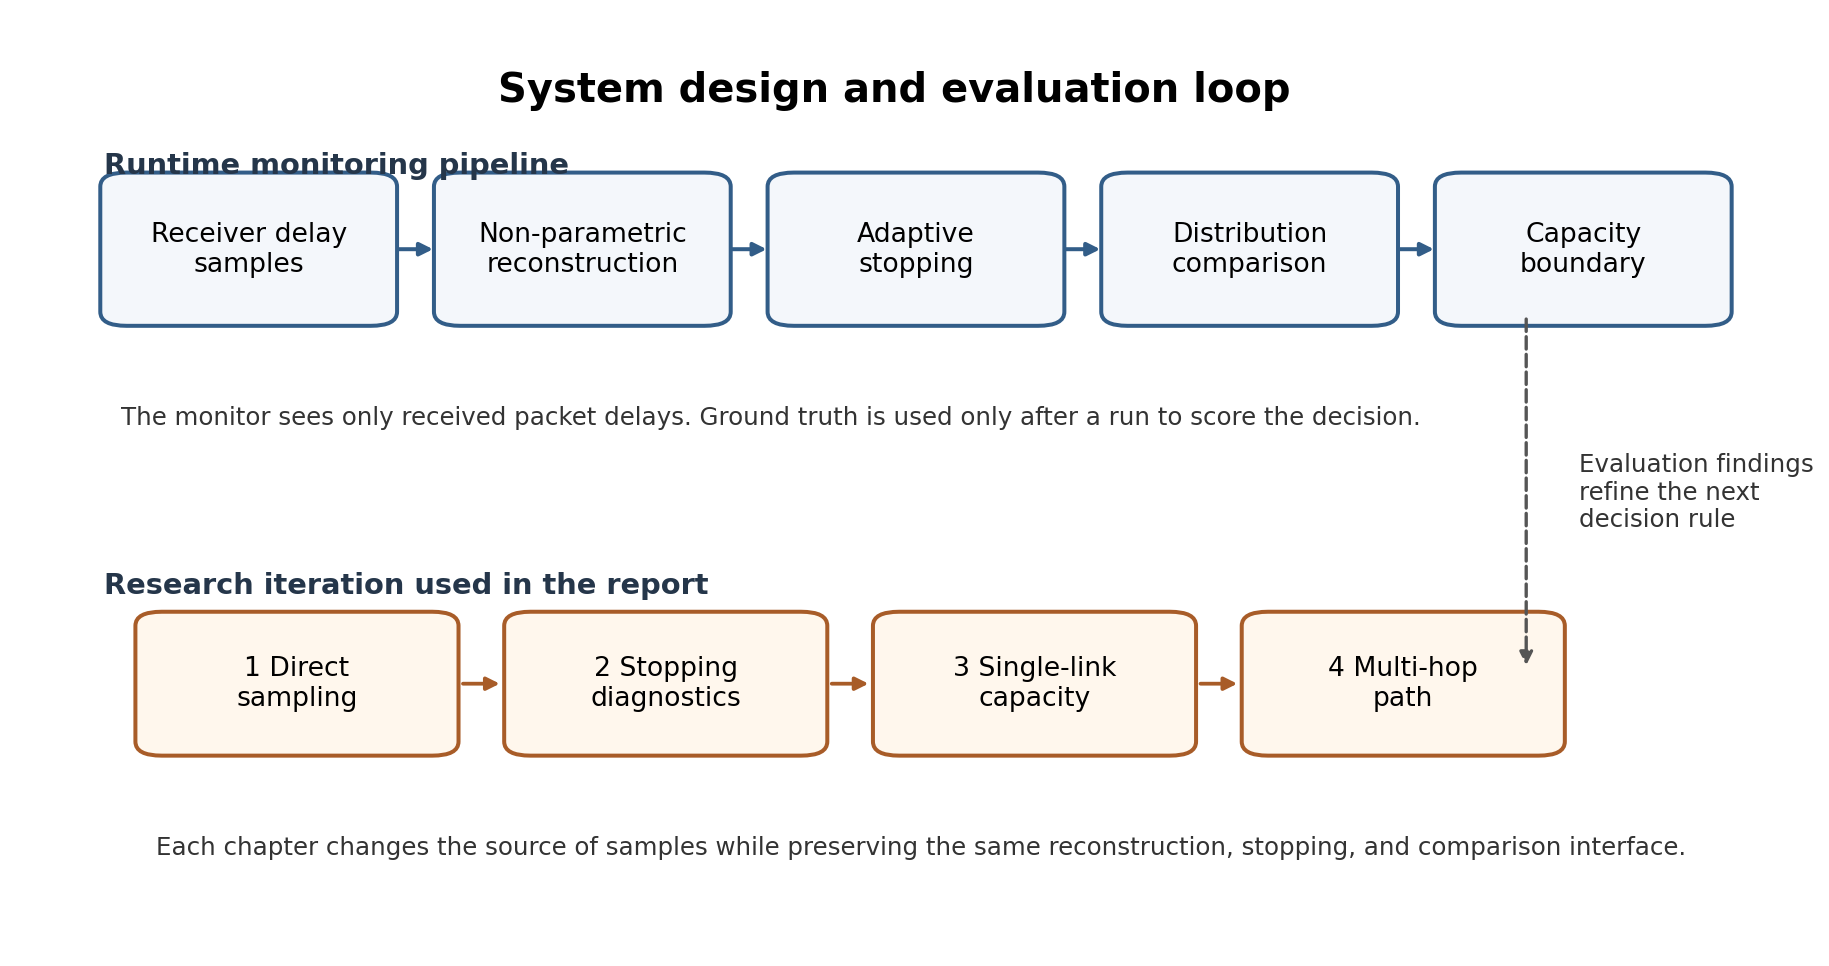
\includegraphics[width=\textwidth]{system_design_iteration.png}
\caption{System pipeline and evaluation decomposition. Runtime monitoring uses only receiver-side delay samples; simulator configuration is used only after each run for scoring. The evaluation isolates reconstruction, stopping, and capacity interpretation before increasing network complexity.}
\label{fig:system-design-iteration}
\end{figure}

The design bridges this chapter and the statistical evaluation that follows. The use case defines what the monitor is trying to do, but it does not yet prove that the first block in the pipeline is reliable. Chapter 3 therefore asks the narrower question of how many samples are needed to reconstruct a delay distribution at all. Chapter 4 then asks when the reconstruction can stop without access to ground truth. Only after those two questions are answered does it become meaningful to interpret a distributional difference as a capacity signal.

\section{Implementation and reproducibility}

The implementation consists of Network Simulator 3 (NS-3) 3.46 simulation programs for the single-link, multi-hop, heterogeneous-link, bursty-traffic, and multi-path input-generation experiments, together with Python analysis scripts for empirical probability mass function reconstruction, kernel density estimation, adaptive stopping, total variation distance computation, scalar baselines, response-rate detection, modal splitting, and plotting. The main simulation code lives under the repository's delay-monitoring experiment directories, while the analysis and plotting scripts live under the corresponding analysis directory. The reported network experiments use fixed seed ranges, a documented load grid, finite first-in, first-out queues, a one millisecond delay grid from 0 to 150 milliseconds, and saved seed-level outputs so that figures and summary tables can be regenerated from the experiment logs.

\section{Operational setting}

Consider a source sending traffic to a destination over a path with unknown remaining capacity. The operator can introduce a controlled offered load for measurement, or can observe naturally increasing traffic, but the monitoring algorithm sees only the packet-delay samples that arrive at the receiver. At each load level \(r_i\), samples are collected until adaptive stopping declares the reconstructed delay distribution stable. The resulting estimate is denoted \(\widehat{P}_{r_i}\). The stopping decision uses only consecutive reconstructions at the same load level; it does not use the true distribution.

After stopping, the current distribution is compared with the first low-load distribution in the evaluated experiments. The comparison uses total variation distance (TVD) as follows.
\[
d_{\mathrm{TV}}\left(\widehat{P}_{r_0},\widehat{P}_{r_i}\right)
= \frac{1}{2}\sum_x
\left|\widehat{P}_{r_0}(x)-\widehat{P}_{r_i}(x)\right|.
\]
If the distance is at most a chosen identity threshold \(\Delta\), the new load is treated as part of the same delay regime. If the distance exceeds \(\Delta\), the load is treated as the first evidence that the path has entered a different regime. This is a batch-level distribution comparison. It is not a test of whether an individual packet belongs to a distribution.

The operational interpretation is conservative. A significant distributional change does not by itself prove that every packet is congested, nor does it identify a physical queue. It indicates that the delay process observed by the receiver no longer matches the low-load operating state. In the capacity use case, the later evaluation asks whether the response to added load accelerates enough to mark a capacity-relevant boundary.

\section{Initial search design and response sweep}

The first design used a two-phase search. The first phase was exponential. Starting from a small offered load \(r_0\), the monitor collected a stopped distribution and then tested \(2r_0,4r_0,8r_0\), and so on. Each new stopped distribution was compared with the low-load stopped distribution. This phase avoided spending many experiments far below the capacity boundary, where distributions were expected to remain similar. It ended once the first significant distributional change was detected, creating a bracket \([r_{\mathrm{safe}},r_{\mathrm{changed}}]\).

The second phase refined the bracket by binary search. The midpoint load was tested, a stopped distribution was reconstructed, and the same distributional comparison was applied. If the midpoint remained similar to the low-load state, it became the new lower end of the bracket. If it was significantly different, it became the new upper end. The output was therefore not a single exact value. It was a capacity range defined by the final stable load and the final changed load. Reporting a range better reflects measurement uncertainty than reporting a point estimate because the boundary is inferred from noisy packet observations and a chosen threshold \(\Delta\).

The evaluated experiments replace this bracketed search with an additive load sweep. The bracketed procedure was the initial deployment-oriented design, but it hides the response curve and would make it harder to see why first-change detection fails. The additive sweep is less efficient as a deployment procedure, but it is more revealing experimentally because it exposes the full response curve. Instead of treating any distributional change as capacity, the final evaluated procedure follows the rate at which TVD changes as load is increased. Delay distributions can move gradually under additional load before the path reaches a capacity-relevant boundary. The useful signal is the point where the distributional response accelerates, not the first point where it is non-zero.

This use case depends directly on the earlier statistical sections. Sample-complexity analysis explains why enough samples are needed before a distribution comparison is meaningful. Adaptive stopping decides when those samples have accumulated at a particular load level. Distribution identity then turns the stopped estimate into an operational decision. Without stopping, the search could compare unstable distributions. Without identity testing, the search would have no principled way to decide whether a new load had changed the path.

\begin{figure}[htbp]
\centering
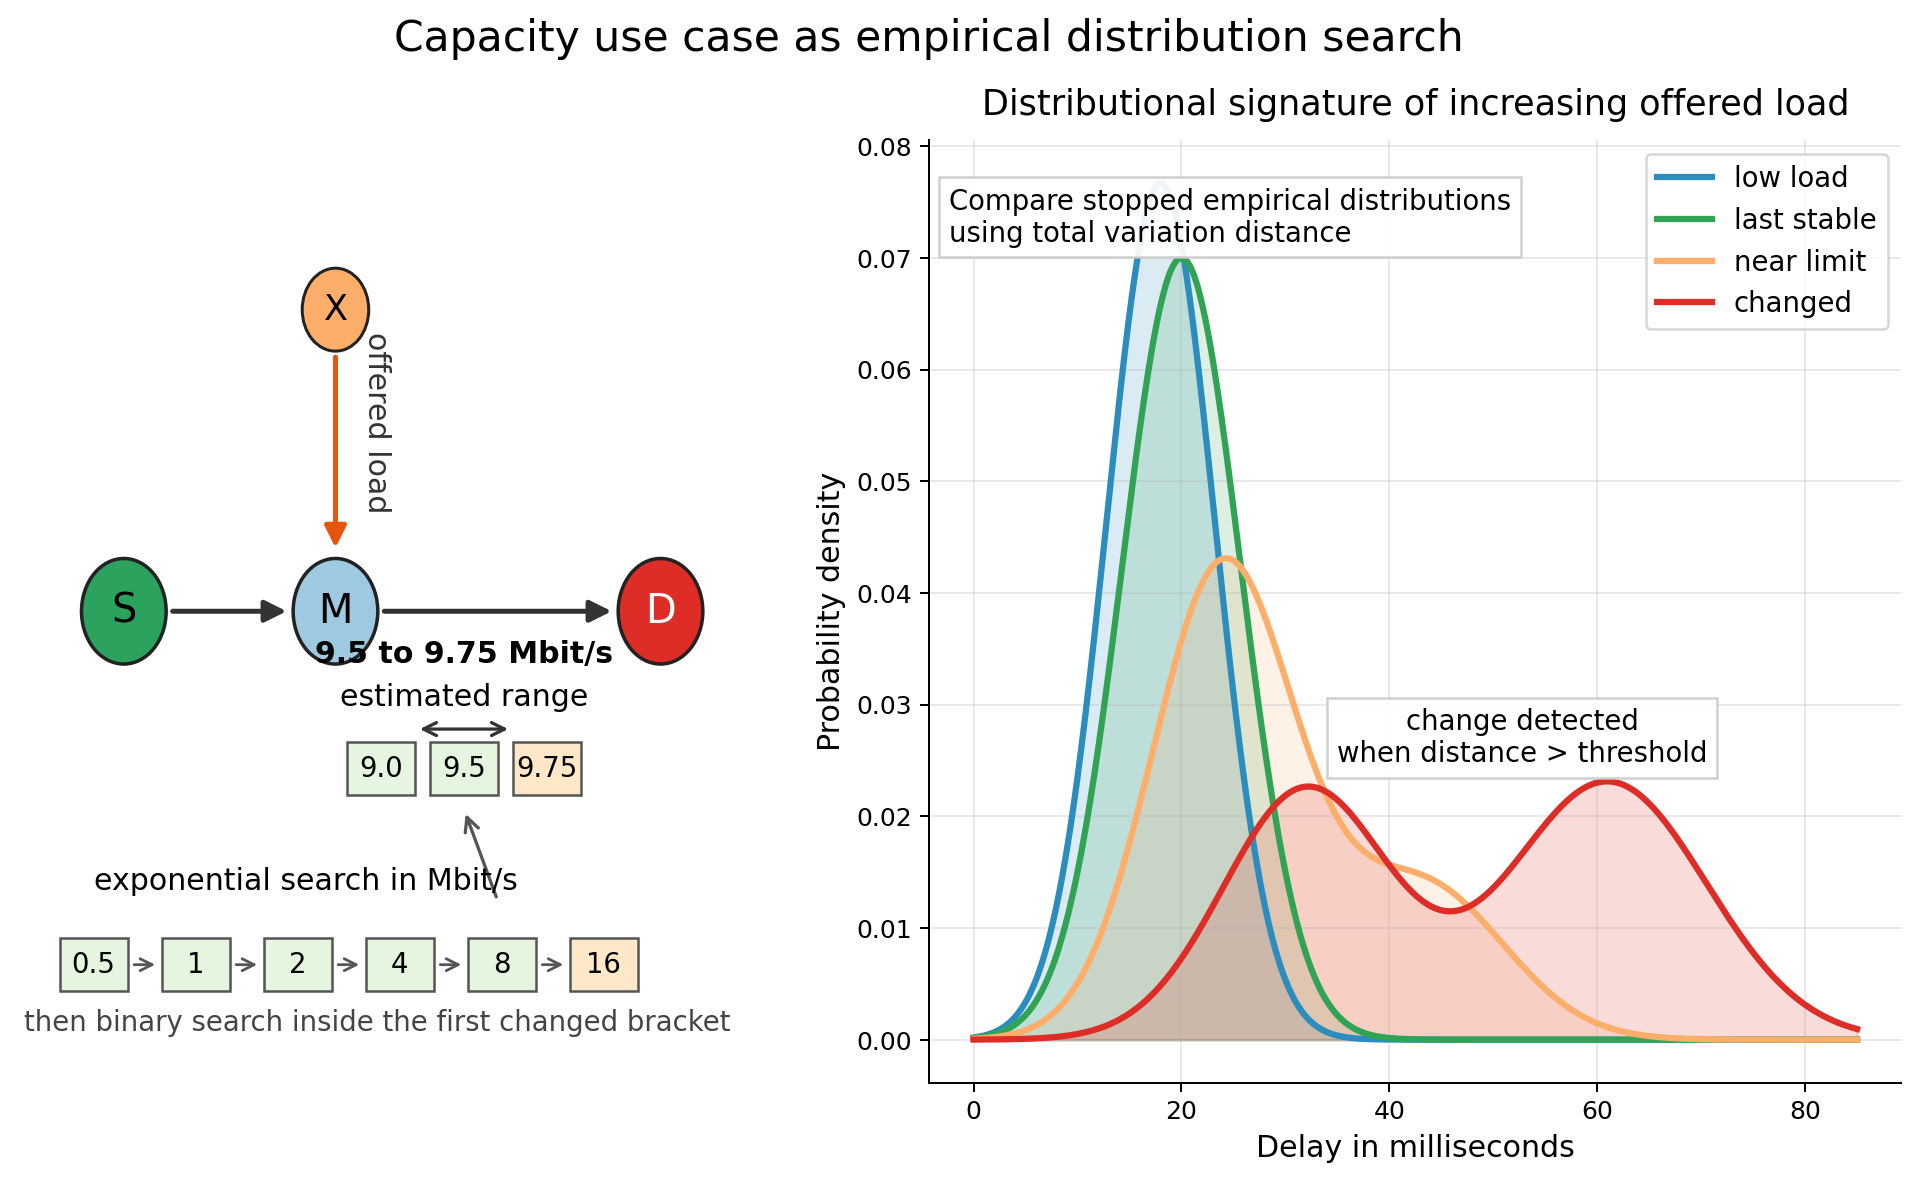
\includegraphics[width=\textwidth]{capacity_use_case_overview.png}
\caption{Early design iteration for bracketed distribution search. The monitor increases offered load until a stopped delay distribution differs from the low-load state and then refines the bracket by binary search. The evaluated runs in Chapters 5 to 7 use additive TVD response tracking instead.}
\label{fig:capacity-use-case-overview}
\end{figure}

\section{Illustrative example}

Figure \ref{fig:capacity-use-case-overview} illustrates the initial bracketed logic using a simple one-link experiment. The configured simulation capacity is 10 megabits per second (Mbit/s), but the monitor does not use this value. It begins at 0.5 Mbit/s and compares stopped empirical distributions at 1, 2, 4, and 8 Mbit/s with the low-load reference. In the example trace, these comparisons remain below the identity threshold, so 8 Mbit/s becomes the highest stable load. The next exponential step, 16 Mbit/s, produces a large distributional change. The search has therefore bracketed the transition between 8 and 16 Mbit/s.

Binary search then tests the interior of the bracket. Loads of 12 Mbit/s and 10 Mbit/s are changed relative to the low-load state, while 9 Mbit/s and 9.5 Mbit/s remain similar. A final test at 9.75 Mbit/s crosses the identity threshold. The resulting estimate is the interval from 9.5 to 9.75 Mbit/s. The configured 10 Mbit/s capacity is used only after this procedure to evaluate the estimate. The example is intentionally simple, but it captures the main point that the capacity boundary is inferred from where the delay distribution changes, not from direct access to the link rate.

The right-hand side of Figure \ref{fig:capacity-use-case-overview} shows why a distributional view is useful. A low-load and a later stable distribution may have similar centres and tails. As the load approaches the limit, the distribution can widen or develop a heavier tail before a scalar threshold becomes decisive. Once the path is pushed beyond its stable regime, the distribution may shift sharply, become multi-modal, or place much more mass at high delays. These shape changes are precisely the information that a scalar mean or a single percentile can hide.

\section{Relationship to active probing}

The use case resembles active probing because the experiment changes offered load. Its interpretation is different. Traditional available-bandwidth tools transmit probe streams and infer a rate from how those probes are dispersed or delayed \cite{jainDovrolisPathload,dovrolisPacketDispersion}. Here, the object being tracked is the empirical delay distribution at each operating point. The monitor is passive with respect to its measurement object: it does not inject dedicated probes or use queue telemetry to make the distributional decision. The evaluation uses controlled load changes only to expose the response curve and score the decision against known simulation capacity.

This framing also differs from fine-grained queue telemetry. ConQuest gives direct visibility into which flows contribute to queue occupancy when programmable data-plane support or link tapping is available \cite{chenConQuest}. The approach here assumes a weaker measurement interface. It does not require the monitor to inspect queue internals or identify the flow responsible for a backlog. It asks whether the end-to-end delay distribution has changed, which is a less detailed but more generally available signal.

PIRATE is closer in spirit because it extracts latency information passively from packet timing under difficult visibility conditions \cite{shobhanaPirate}. The difference is the unit of inference. PIRATE estimates response latency from causal request pairs. The method studied here estimates a distribution over packet delays and asks whether that distribution has changed under load. Both approaches show the value of packet timing beyond simple counters, but they answer different operational questions.

The use case provides the bridge between the statistical foundations and the later network experiments. A successful result would not mean that the exact physical capacity has been measured. It would mean that the monitoring system can identify the range of offered load over which the path leaves its previous delay regime. The following chapters make that test progressively harder: first a single link, then a longer one-route path, and finally a multi-path mixture in which several route behaviours appear in the same receiver-side distribution.


\chapter{Statistical Sample Complexity}
\label{sec:eval-statistical}

Sample-complexity analysis provides the statistical foundation for the rest of the project. Later use-case experiments aim to infer remaining path capacity from changes in the observed delay distribution, but that objective depends on a prior capability: the monitor must be able to reconstruct a distribution accurately without being told its generating family. To isolate that requirement, the network simulator is removed from the loop and samples are drawn directly from known distributions. The experiment is intentionally narrow. Its value is that any failure would point to the statistical reconstruction method itself, rather than to Network Simulator 3 (NS-3), packet scheduling, or topology design.

Only samples are exposed to the monitor. It is not told whether they came from a binomial, Zipfian, piecewise, normal, lognormal, or Weibull distribution. The generating family creates ground truth for evaluation, but plays no role in reconstruction. Maintaining that separation is essential because the eventual capacity use case must also be distribution-agnostic. A path may move from a low-delay state to a congested state by changing its skew, tail, or modality rather than by following a named parametric family.

Accuracy is measured primarily by total variation distance (TVD). For a true distribution \(P\) and an estimate \(\widehat{P}\) over a finite domain \(\mathcal{X}\), this is
\[
d_{\mathrm{TV}}(P,\widehat{P}) =
\frac{1}{2}\sum_{x \in \mathcal{X}} |P(x)-\widehat{P}(x)|.
\]
A reconstruction is treated as successful when this distance is at most a target error \(\delta\), with failure probability at most \(\varepsilon\). Throughout this section, \(\delta=0.05\) and \(\varepsilon=0.05\), so the target is TVD of at most 0.05 with probability at least 0.95.

The section answers three evaluation questions in order. First, it checks where the finite-sample reference bound comes from and how it should be interpreted. Second, it applies the bound to discrete distributions, where the support is already finite. Third, it applies the same comparison to continuous delay distributions after discretising them onto a common evaluation grid. The order follows the theory. The TVD learning bound is stated for a finite domain of \(k\) outcomes, so the first experiment uses native discrete supports where those outcomes are exactly defined. The continuous experiment then maps delay samples onto a 150-bin grid, which is the finite-domain form used by the later network evaluation.

\section{The Learning Bound}

Finite-domain distribution learning supplies the theoretical reference point. Canonne's monograph on distribution testing records this as the learning baseline for arbitrary distributions on a known finite domain, and uses it as the benchmark against which sublinear testing algorithms are compared \cite{canonneTopics}. Canonne writes the TVD tolerance as \(\varepsilon\) and the failure probability as \(\delta\). Using this report's notation, where \(\delta\) is the TVD target and \(\varepsilon\) is the failure probability, independent samples from an unknown distribution over \(k\) possible outcomes are sufficient for the plug-in histogram estimator to learn the distribution in TVD with sample complexity
\[
n = \Theta\left(\frac{k+\log(1/\varepsilon)}{\delta^2}\right).
\]
This information-theoretic finite-sample bound is tight up to universal constants for arbitrary distributions on \(k\) categories \cite{canonneShort,canonneTopics,devroyeLugosi}. The base of the logarithm affects only constants in the asymptotic theorem; the numerical calculations below use the natural logarithm. The \(k\) term counts how many probabilities must be estimated. The \(1/\delta^2\) term comes from concentration, so halving the desired error requires roughly four times as many samples. The \(\log(1/\varepsilon)\) term pays for high probability rather than only average-case accuracy.

As a baseline, the bound suits this first evaluation because the question is reconstruction rather than capacity identification. Later sections use the reconstructed distribution to compare path states, but this section keeps that later decision out of scope and measures only TVD against the known generating distribution.

Finiteness is also a methodological constraint. A discrete distribution already has a finite support. A continuous delay distribution must be evaluated on a finite grid before TVD can be computed as a sum. The grid is the discretisation used for evaluation, not a claim that observations are aggregated over time. A bin is one fixed interval on the delay axis. In the continuous experiments below, one bin corresponds to a one millisecond interval, and all bins from 0 milliseconds to 150 milliseconds are used. This gives \(k=150\) categories. Once the continuous distribution has been converted into bin probabilities, the same finite-domain comparison applies.

The experiments use the explicit reference value
\[
n_{\mathrm{ref}} =
\left\lceil \frac{k+\log(1/\varepsilon)}{\delta^2} \right\rceil .
\]
This reference drops the unknown asymptotic constant hidden by the \(\Theta(\cdot)\) notation, so it is an order-of-magnitude comparison scale rather than a formal sufficient-sample threshold. With \(\varepsilon=0.05\), \(\log(1/\varepsilon)=\log(20)=2.996\). The corresponding reference curve in the plots is the same relationship inverted as
\[
\delta_{\mathrm{ref}}(n)=
\sqrt{\frac{k+\log(1/\varepsilon)}{n}}.
\]
The curve is a distribution-free reference, not a prediction that every structured distribution will need exactly that many samples. The empirical questions are whether TVD falls with \(n\), whether harder shapes converge more slowly, and how far below \(n_{\mathrm{ref}}\) the target is reached for each shape. Empirical failure probability is measured as the fraction of seeds whose reconstruction misses the TVD target, which is the empirical analogue of the \(\varepsilon\) parameter in the bound.

\begin{figure}[htbp]
\centering

\includegraphics[width=\textwidth]{statistical_distribution_shapes.png}
\caption{Ground-truth distributions used in the direct-sampling sample-complexity evaluation. The top row shows the three discrete probability mass functions. The bottom row shows the three continuous densities.}
\label{fig:statistical-distribution-shapes}
\end{figure}

\section{Discrete Sampling}

Three finite distributions are used in the discrete experiment, shown in the top row of Figure \ref{fig:statistical-distribution-shapes}. They are chosen so that support size and probability shape can be examined separately, with each shape standing in for a feature that can also appear in real delay distributions. A binomial distribution gives a smooth, concentrated peak, resembling a lightly loaded path with narrow delay variation. A Zipfian distribution gives strong skew and a long finite tail, matching the case where delays are usually small but occasionally much larger. A piecewise distribution gives irregular, multi-modal mass, as would be expected when delays arise from several disjoint regimes such as different service classes or route choices. The purpose of the discrete experiment is not to claim that delay is intrinsically discrete. It asks whether reconstruction can preserve these shape features before the added complication of continuous sampling.

The binomial case uses
\[
X \sim \mathrm{Binomial}(20,0.5),
\qquad
p(x)=\binom{20}{x}0.5^x0.5^{20-x},
\qquad x \in \{0,\ldots,20\}.
\]
The support has \(k=21\) possible outcomes. The Zipfian case uses a truncated power law,
\[
p(x)=\frac{x^{-1.5}}{\sum_{j=1}^{20}j^{-1.5}},
\qquad x \in \{1,\ldots,20\},
\]
so \(k=20\). Finally, the piecewise case also uses support \(\{1,\ldots,20\}\), with probabilities indexed in support order as
\[
\begin{aligned}
p = (&0.12,0.02,0.08,0.01,0.10,0.03,0.07,0.12,0.02,0.09,\\
     &0.01,0.08,0.04,0.06,0.02,0.05,0.02,0.04,0.01,0.01).
\end{aligned}
\]
These values sum to one and create separated high-probability regions.

For each distribution, samples are drawn directly from the probability mass function (PMF) and reconstructed using the empirical PMF. Each point in Figure \ref{fig:statistical-discrete-tvd} is the median TVD over 100 random seeds, while the shaded band shows the interquartile range. The median shows the typical reconstruction trajectory, while the interquartile band shows whether the conclusion is being driven by a narrow group of seeds or by consistent behaviour across runs. The adaptive stopping section therefore reports correctness across seeds explicitly, since an operational monitor should care about the probability of stopping with a bad reconstruction. Tested sample sizes are centred around the calculated \(n_{\mathrm{ref}}\) value for each support size.

\begin{figure}[htbp]
\centering
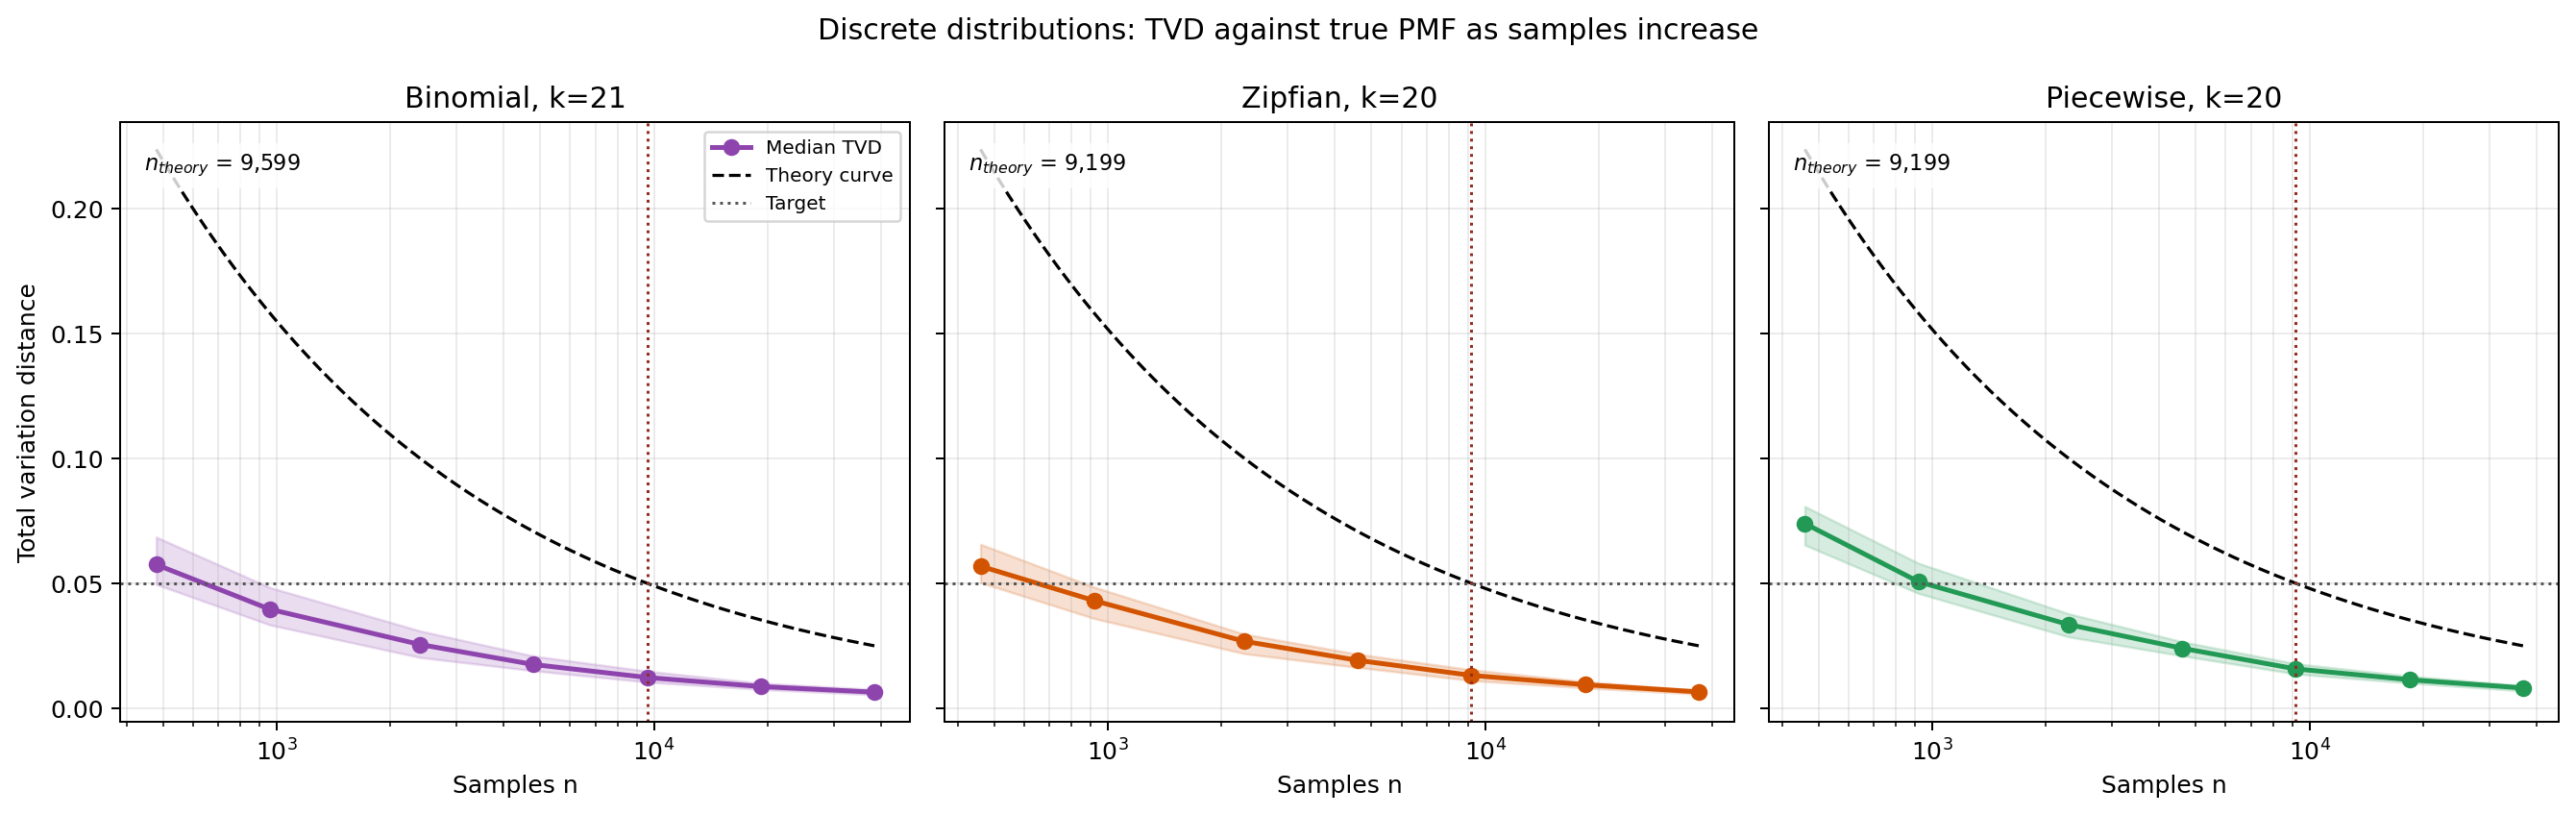
\includegraphics[width=\textwidth]{statistical_discrete_tvd_vs_n.png}
\caption{Discrete reconstruction error as the sample count increases. The dotted horizontal line is the target \(\delta=0.05\), the red vertical line is the calculated \(n_{\mathrm{ref}}\), and the dashed black curve is \(\delta_{\mathrm{ref}}(n)\).}
\label{fig:statistical-discrete-tvd}
\end{figure}

\begin{table}[htbp]
\centering
\small
\begin{tabular}{lrrrr}
\toprule
Distribution & \(k\) & \(n_{\mathrm{ref}}\) & Target \(n\) & TVD at \(n_{\mathrm{ref}}\) \\
\midrule
Binomial & 21 & 9,599 & 960 & 0.0123 \\
Zipfian & 20 & 9,199 & 920 & 0.0132 \\
Piecewise & 20 & 9,199 & 2,300 & 0.0158 \\
\bottomrule
\end{tabular}
\caption{Discrete sample-complexity results. The first \(n\) column reports the smallest tested sample count for which the median TVD is below 0.05.}
\label{tab:statistical-discrete-results}
\end{table}

For the binomial case,
\[
n_{\mathrm{ref}} =
\left\lceil \frac{21+\log(20)}{0.05^2} \right\rceil
=
\left\lceil \frac{23.996}{0.0025} \right\rceil
= 9{,}599.
\]
For the Zipfian and piecewise cases, \(k=20\), so
\[
n_{\mathrm{ref}} =
\left\lceil \frac{20+\log(20)}{0.05^2} \right\rceil
=
\left\lceil \frac{22.996}{0.0025} \right\rceil
= 9{,}199.
\]

Figure \ref{fig:statistical-discrete-tvd} shows the expected decrease in TVD as \(n\) grows. Binomial and Zipfian estimates reach the 0.05 target with about ten times fewer samples than \(n_{\mathrm{ref}}\), while the piecewise estimate reaches it with about four times fewer. More important than the absolute gap to theory is the ranking across distributions. Binomial is easiest despite having one more support point than the other two cases, because most probability mass is concentrated near the centre and the low-probability tails contribute little to TVD. It first reaches the target at \(n=960\), and by \(n_{\mathrm{ref}}=9{,}599\) the median TVD is 0.0123.

Zipfian reaches the target at \(n=920\) and has median TVD 0.0132 at its reference point. Its head is easy to estimate because the first few outcomes carry most of the mass. Rare tail outcomes are harder individually, but their combined probability is limited, so tail errors do not dominate TVD. That is why the Zipfian curve stays close to the binomial curve despite having a more uneven shape.

Piecewise is the hardest discrete case. It needs \(n=2{,}300\) samples before median TVD falls below 0.05, roughly two and a half times the binomial requirement at a similar support size. Probability mass is spread across separated peaks and troughs, so the empirical PMF has to learn several non-neighbouring support points accurately. The result shows that the theoretical bound is conservative even outside the smooth cases. An irregular finite distribution still reaches the target before the calculated distribution-free sample count, but it does so later than the smoother and more skewed alternatives.

Support size \(k\) alone does not determine practical reconstruction difficulty; the arrangement of mass across the support matters as well. Piecewise therefore remains in the adaptive stopping experiments as a stronger stress test for false stability than binomial. A rule that succeeds only on smooth or highly concentrated shapes has not yet shown that it can handle the irregular probability mass that appears in multi-regime delay behaviour.

\section{Continuous Sampling}

Continuous sampling uses the normal, lognormal, and Weibull distributions shown in the bottom row of Figure \ref{fig:statistical-distribution-shapes}. These families are not claimed to exhaustively model Internet delay. They provide controlled representatives of shape classes that matter for passive monitoring. Empirical work on network delay reports concentrated modes with right-skewed or heavy-tailed variation, and has fitted gamma, lognormal, and Weibull forms to one-way delay and round-trip time measurements \cite{karakasDelay}. Wider traffic-modelling studies also use lognormal and Weibull families for Internet metrics and packet-level behaviour \cite{downeyLognormal,arfeenWeibull}. Normal is included as a symmetric low-variance baseline. Lognormal captures a positive, right-skewed regime in which delay is usually small but occasionally much larger. Weibull gives a different positive asymmetric shape, with a sharp rise and a longer decaying tail. Together, the three families test whether reconstruction works beyond a single benign, bell-shaped case.

The parameter choices are
\[
X_{\mathrm{normal}} \sim \mathcal{N}(40,2^2),
\qquad
\log X_{\mathrm{lognormal}} \sim \mathcal{N}(2.3,0.2^2),
\qquad
X_{\mathrm{weibull}} \sim \mathrm{Weibull}(\lambda=10,\alpha=2).
\]
All samples are evaluated on the same one millisecond grid from 0 milliseconds to 150 milliseconds. This grid is the finite representation used to compare continuous objects. True bin probabilities are computed by integrating the known cumulative distribution function over each bin. The empirical PMF counts sample frequencies on the same grid. The kernel density estimate (KDE) uses a Gaussian kernel with bandwidth chosen by Scott's rule, which is the default in the SciPy implementation used throughout the project. Scott's rule sets the bandwidth from the sample size and standard deviation alone, so it does not require knowledge of the generating family. The KDE is evaluated at the bin centres and normalised for comparison as a probability mass function on the same grid. TVD is then computed over probability mass on the grid, not over raw continuous density values.

The finite-grid comparison has \(k=150\), roughly an order of magnitude larger than the discrete supports above, so the calculated reference value is
\[
n_{\mathrm{ref}} =
\left\lceil \frac{150+\log(20)}{0.05^2} \right\rceil
=
\left\lceil \frac{152.996}{0.0025} \right\rceil
= 61{,}199.
\]
Each point in Figure \ref{fig:statistical-continuous-tvd} is the median across 30 random seeds, with interquartile shading. The main text keeps the combined view because it shows the ordering between the three continuous families. The individual normal and lognormal curves are reported in Appendix Figures \ref{fig:app-tvd-vs-n-normal} and \ref{fig:app-tvd-vs-n-lognormal}, while the Weibull curve is also retained in Appendix Figure \ref{fig:app-tvd-vs-n-weibull} as the hardest continuous reconstruction.

\begin{figure}[htbp]
\centering

\includegraphics[width=\textwidth]{statistical_continuous_tvd_vs_n.png}
\caption{Continuous reconstruction error on the one millisecond grid. The PMF line compares the binned empirical distribution with the true bin probabilities. The KDE line compares the smoothed estimate with the same true bin probabilities.}
\label{fig:statistical-continuous-tvd}
\end{figure}

\begin{table}[htbp]
\centering
\small
\begin{tabular}{lrrrrr}
\toprule
Distribution & PMF target \(n\) & KDE target \(n\) & PMF at reference & KDE at reference & Gap \\
\midrule
Normal & 500 & 500 & 0.0047 & 0.0060 & 0.0031 \\
Lognormal & 1,000 & 500 & 0.0052 & 0.0057 & 0.0030 \\
Weibull & 2,000 & 500 & 0.0073 & 0.0058 & 0.0039 \\
\bottomrule
\end{tabular}
\caption{Continuous sample-complexity results on the one millisecond grid. The first \(n\) columns report the smallest tested sample count for which the median TVD is below 0.05. The last three columns report median values at \(n_{\mathrm{ref}}=61{,}199\).}
\label{tab:statistical-continuous-results}
\end{table}

Figure \ref{fig:statistical-continuous-tvd} shows the same broad pattern as the discrete results. TVD falls as sample count grows, and all three distributions are well below the target by the calculated \(n_{\mathrm{ref}}\). The empirical PMF reaches the target at 500 samples for normal, 1,000 samples for lognormal, and 2,000 samples for Weibull. Normal places most mass in a narrow symmetric region, so the important bins are quickly populated. Lognormal skew makes the right tail noisier. Weibull is hardest for the binned PMF because its mass rises sharply near the lower end and then decays over a longer range, requiring the histogram to estimate both a peak and a tail.

KDE changes the low-sample regime. It reaches the 0.05 target at the first tested point, 500 samples, for all three continuous distributions. This does not mean KDE has been given the parametric family; it uses only the local smoothness of nearby delay values. Where the empirical PMF treats adjacent one millisecond bins as unrelated categories, KDE shares information across neighbouring values. Smoothing is especially helpful for Weibull: at 500 samples, the PMF median TVD is 0.0875, while the KDE median TVD is 0.0421. The later continuous experiments therefore use KDE as the primary estimator and retain the binned PMF as a finite-grid audit.

The conservative reading is slightly more nuanced than the median alone. For the binned PMF, the first sample count whose median is below 0.05 is not always the first point whose upper quartile is also below 0.05. Normal and lognormal PMF estimates have median TVD below the target at 500 samples, but their upper quartiles remain above it; by 1,000 samples the interquartile band is safely below the target. For KDE, the upper quartile is already below 0.05 at 500 samples for all three continuous families. The later stopping analysis therefore uses correctness over seeds rather than only median stopping time.

At the reference point, both estimators are much more accurate than required. Binned PMF medians are 0.0047 for normal, 0.0052 for lognormal, and 0.0073 for Weibull. KDE medians are 0.0060, 0.0057, and 0.0058. The small reversal for normal and lognormal, where PMF is slightly closer than KDE at very large \(n\), is expected. Once many samples have populated the bins, the empirical PMF has little variance left, while KDE still introduces a small amount of smoothing bias. KDE is more sample efficient at the target accuracy used here, while PMF becomes competitive once the sample count is already large.

The comparison fixes the estimator choice for the next iteration. KDE is used for early continuous reconstruction because it buys sample efficiency without using a parametric assumption. PMF remains useful as a finite-grid audit because it shows what can be learned without smoothing. The small large-\(n\) KDE bias also prevents over-interpretation of the smoother curve. Smoothing helps early stopping, but it should not be treated as ground truth when the use case needs a conservative capacity decision.

The supporting KDE-versus-PMF diagnostic in Appendix Figure \ref{fig:app-estimator-gap} checks that smoothing is not reconstructing a fundamentally different object. The gap between the binned PMF and KDE falls with \(n\), with the largest small-sample disagreement in the Weibull case and much smaller gaps for normal and lognormal. That agreement is important for the use case. A capacity estimator based on distributional change should not depend on an arbitrary choice between two incompatible representations of the same samples.

The finite-domain reference captures the dependence on support size, confidence, and error tolerance, and the empirical curves behave as the theory predicts. Structured distributions reach the 0.05 target with one to two orders of magnitude fewer samples than \(n_{\mathrm{ref}}\). Continuous KDE estimates reach it at 500 samples for all three families, against \(n_{\mathrm{ref}}=61{,}199\), a factor of about 122. Discrete PMF estimates reach it between \(n=920\) and \(n=2{,}300\), against \(n_{\mathrm{ref}}\) values near 9{,}200, a factor between 4 and 10. Smoothness, concentration, skew, and modality each shift this gap, with piecewise and Weibull the slowest of the six tested distributions. An online monitor that waited for \(n_{\mathrm{ref}}\) packets every time would therefore over-collect by roughly that factor, motivating the adaptive stopping rule in the next section.

Because this evaluation uses stationary distributions and direct sampling, it does not yet test how the same estimators behave on non-stationary delay traces or under network-induced effects such as missing or reordered observations. Those tests belong to the network experiments. The reading at this stage is that reconstruction itself is not the bottleneck. If a later network experiment fails, the likely cause is the stopping rule, the network mechanism, or the identification step rather than the empirical PMF or KDE estimator.

Appendix \ref{app:statistical-diagnostics} contains the delta-sweep, bin-resolution, KDE-disagreement, and Kolmogorov-Smirnov diagnostics. They support the same conclusion from a wider set of views. Stricter TVD targets and finer grids increase the theoretical sample requirement, while the structured distributions tested here usually converge much earlier than the worst-case finite-domain reference. The Kolmogorov-Smirnov diagnostics are secondary because the main reconstruction and identity decisions use TVD. Kolmogorov-Smirnov distance is sensitive to the maximum vertical gap between cumulative distributions, whereas TVD measures total probability-mass disagreement across the delay grid. The plots therefore check that convergence is not only a TVD-specific artefact; they do not choose the operating point. Wasserstein distance, also known as earth mover's distance, remains a useful future diagnostic because it measures how far probability mass moves along the delay axis.

\clearpage

\chapter{Adaptive Stopping}
\label{sec:eval-adaptive}

Adaptive stopping moves the analysis from offline reconstruction to online decision making. The previous section shows that the tested delay distributions can be reconstructed long before the worst-case sample bound. A passive monitor, however, cannot look at ground truth during deployment and cannot know in advance where it sits on the TVD curve. It needs a stopping rule that decides when the current estimate is stable enough to be passed to the next stage of the system. In the use case, that next stage is distribution identity: comparing the current delay distribution with a reference capacity state.

\section{Stopping Rule and Metrics}

At runtime, samples are processed in groups of \(B\) packets, where \(B\) is the packets per batch parameter. After each new group of packets, the monitor computes the TVD between the current estimate and the previous estimate. If this inter-estimate TVD falls below a threshold \(\theta\), the monitor stops:
\[
\tau = \inf\left\{mB : d_{\mathrm{TV}}\left(\widehat{F}_{mB}, \widehat{F}_{(m-1)B}\right) < \theta\right\}.
\]
The true distribution is not used by the stopping rule. Ground truth appears only after a run has stopped, when the experiment checks whether the stopped estimate satisfies \(d_{\mathrm{TV}}(\widehat{F}_{\tau},F)\leq\delta\), where the target is \(\delta=0.05\).

The rule is simpler than classical sequential tests. Sequential probability ratio tests make likelihood-ratio decisions between specified hypotheses, while cumulative-sum methods accumulate evidence for a persistent change in process behaviour \cite{waldSequential,pageCusum,laiSequential}. The monitor here does neither. It has no parametric likelihood, no labelled pre-change and post-change models, and no ground-truth reference distribution at runtime. The stopping rule is therefore a low-cost stability check for an empirical distribution estimate, not a formal sequential change detector. That limitation bounds the claim: the rule is evaluated empirically under the tested distributions rather than given a finite-sample stopping guarantee.

Estimates in this rule are cumulative. With \(B=100\), the first comparison is between the reconstruction from samples 1 to 100 and the reconstruction from samples 1 to 200. The next comparison is between samples 1 to 200 and samples 1 to 300. The rule is therefore not comparing disjoint batches. It asks whether adding another batch changes the accumulated reconstruction enough to justify continuing. Batch size controls the spacing of these decisions: small batches give more opportunities to stop, while larger batches make each stability check less noisy.

The adaptive sweep tests eight choices for packets per batch,
\(B \in \{100,200,300,500,750,1000,1500,2000\}\), and six stability thresholds, \(\theta \in \{\delta/6,\delta/5,\delta/4,\delta/3,\delta/2,\delta\}\). Each configuration is evaluated over 100 random seeds. The threshold \(\theta\) controls how much movement is tolerated between two consecutive cumulative estimates. Setting \(\theta=\delta\) means that the stopping rule accepts an inter-estimate change as large as the final reconstruction-error target itself. Setting \(\theta=\delta/6\) requires the local change to be six times smaller before stopping. This makes \(\theta\) a conservativeness parameter rather than a new accuracy target.

The continuous group uses the same normal, lognormal, and Weibull distributions as the sample-complexity experiment, reconstructed with a Gaussian kernel density estimate (KDE) on the 1 ms grid using Scott's rule for bandwidth selection. The discrete group uses a binomial distribution, a truncated Zipf distribution, and a hand-built multi-modal piecewise distribution over roughly 20 support points, reconstructed with a probability mass function (PMF) estimator. Both groups are retained because they answer different design questions. Continuous KDE reconstruction is the more natural choice for real-valued delays, while discrete PMF reconstruction tests the harder case where probability mass must be allocated to separate support points without smoothing. The final monitoring system may use one representation, but comparing both here shows how much of the stopping behaviour comes from the estimator rather than from the stopping rule alone.

The evaluation asks whether stability between consecutive estimates is a reliable proxy for accuracy against the true distribution. The previous section uses ground truth only to measure when a reconstruction becomes accurate, while a deployed passive monitor sees only its own estimates. A useful stopping rule must therefore stop early and still meet the TVD target with high probability. Since the bound in the previous section asks for failure probability at most \(\varepsilon=0.05\), the empirical analogue here is correctness of at least 0.95 across the seeds at a given stopping configuration.

Small values of \(B\) give the monitor more opportunities to stop, but each decision rests on a small increment of new evidence. Loose thresholds amplify the same problem by accepting weak signs of stability. Continuous and discrete reconstruction are analysed separately because they fail for different reasons. A kernel density estimate can look stable while the smoothed peak or tail is still wrong. A probability mass function estimate can look stable before enough mass has reached separated support points. These are precisely the shape errors that would matter in a capacity use case, where the decision depends on whether the current delay distribution still matches a reference state.

Correctness is the primary adaptive metric, defined as the fraction of seeds where the stopped estimate is within TVD 0.05 of the true distribution. Efficiency is secondary, defined as the ratio between the relevant theoretical bound and the median number of packets collected before stopping. Efficiency is only interpreted as useful when correctness is at least 0.95. Below that point, a high efficiency number means only that the rule stopped early, not that it stopped safely. The figures in the main text are introduced as they become needed. Correctness heatmaps first establish which operating points are reliable. Stopping-count plots then show the packet cost of those choices. The Weibull stopped-distribution and continued-trace plots show what the decision means in distributional terms. Normal and lognormal variants are retained in the appendix so that the section can make the argument without repeating the same visual pattern three times. In Table \ref{tab:packet-timing-reference}, Gbit/s denotes gigabits per second.

\begin{table}[htbp]
\centering
\small
\begin{tabular}{rrrr}
\toprule
Packet count & Time at 100 Gbit/s & Time at 10 Gbit/s & Time at 1 Gbit/s \\
\midrule
200 & 24 microseconds & 240 microseconds & 2.4 milliseconds \\
400 & 48 microseconds & 480 microseconds & 4.8 milliseconds \\
800 & 96 microseconds & 960 microseconds & 9.6 milliseconds \\
1,600 & 192 microseconds & 1.92 milliseconds & 19.2 milliseconds \\
3,000 & 360 microseconds & 3.60 milliseconds & 36.0 milliseconds \\
\bottomrule
\end{tabular}
\caption{Back-to-back transmission time for representative 1500-byte packet counts. These times are only a scale reference, since the passive monitor does not inject traffic.}
\label{tab:packet-timing-reference}
\end{table}

Packet count is reported as the primary cost because the monitor is passive. The time needed to collect a given number of samples depends on the traffic already traversing the path. Table \ref{tab:packet-timing-reference} is therefore only a scale conversion, not an assumption that the monitor sends probes. For 1500-byte packets sent back-to-back on a 100 gigabit per second link, 1,600 packets correspond to about 192 microseconds and 3,000 packets to about 360 microseconds. On a 1 gigabit per second link the same counts correspond to 19.2 milliseconds and 36.0 milliseconds. This makes the sample counts easier to interpret. In a high-rate setting, successful stopping configurations are not waiting for a long measurement interval; they are waiting for enough naturally observed packets to make the distribution stable.

\section{Continuous Stopping Behaviour}

\begin{figure}[htbp]
\centering

\includegraphics[width=\textwidth]{correctness_grid_cont.png}
\caption{Correctness of the adaptive stopping rule for the continuous distributions. Each cell is the fraction of 100 seeds where the stopped estimate is within TVD 0.05 of the true distribution. The vertical axis increases upwards with batch size.}
\label{fig:adaptive-cont-correctness}
\end{figure}

Figure \ref{fig:adaptive-cont-correctness} shows the continuous correctness grid, with larger batch sizes higher on the vertical axis. Unsafe settings concentrate in the lower-right corner, where the monitor checks too often and accepts too much change between estimates. With \(B=100\) and \(\theta=\delta\), correctness is 0.53 for normal, 0.42 for lognormal, and 0.49 for Weibull. The rule accepts inaccurate estimates in roughly half of the trials while appearing highly efficient. Since \(\theta=\delta\) allows consecutive estimates to differ by the full final-error target, the rule can stop even when both estimates are still wrong in the same direction. Tightening the threshold to \(\theta=\delta/6\) at the same value of \(B\) raises correctness to 0.98, 0.95, and 0.97. Increasing \(B\) has a similar stabilising effect because each comparison is made after a larger cumulative sample. At \(B=200\) and \(\theta=\delta/6\), correctness is 1.00 for normal, 1.00 for lognormal, and 0.99 for Weibull. The heatmap therefore does not imply that smaller batches are always bad. It shows that the monitor needs enough evidence between decisions for stability to be meaningful.

The Weibull case is retained as the continuous stress case because it was the hardest continuous distribution for the binned PMF in the sample-complexity evaluation. Its sharp rise and longer right tail make it a useful check on whether KDE stability is hiding a shape error. The most aggressive setting, \(B=100\) and \(\theta=\delta\), stops after a median of 200 packets but is correct in only 49 percent of seeds. Tightening the threshold to \(\theta=\delta/6\) at the same batch size raises correctness to 97 percent, while \(B=200,\theta=\delta/6\) reaches 99 percent correctness with a median stopping time of 1,400 packets. Appendix Figures \ref{fig:adaptive-weibull-efficiency}, \ref{fig:app-adaptive-normal-efficiency}, and \ref{fig:app-adaptive-lognormal-efficiency} give the corresponding heatmaps.

Packet-count diagnostics are kept in Appendix Figures \ref{fig:n-stop-summary-cont-all} and \ref{fig:n-stop-b200-continuous}. The main point is that larger values of \(B\) and tighter thresholds increase stopping time, but the conservative operating point remains far below the finite-domain reference. At \(B=200,\theta=\delta/6\), median stopping counts are 1,600 packets for normal and lognormal, and 1,400 packets for Weibull, with correctness values of 1.00, 1.00, and 0.99. This gives the use case a cleaner input: a distribution estimate held to a stricter stability standard before any capacity interpretation is made.

\begin{figure}[htbp]
\centering
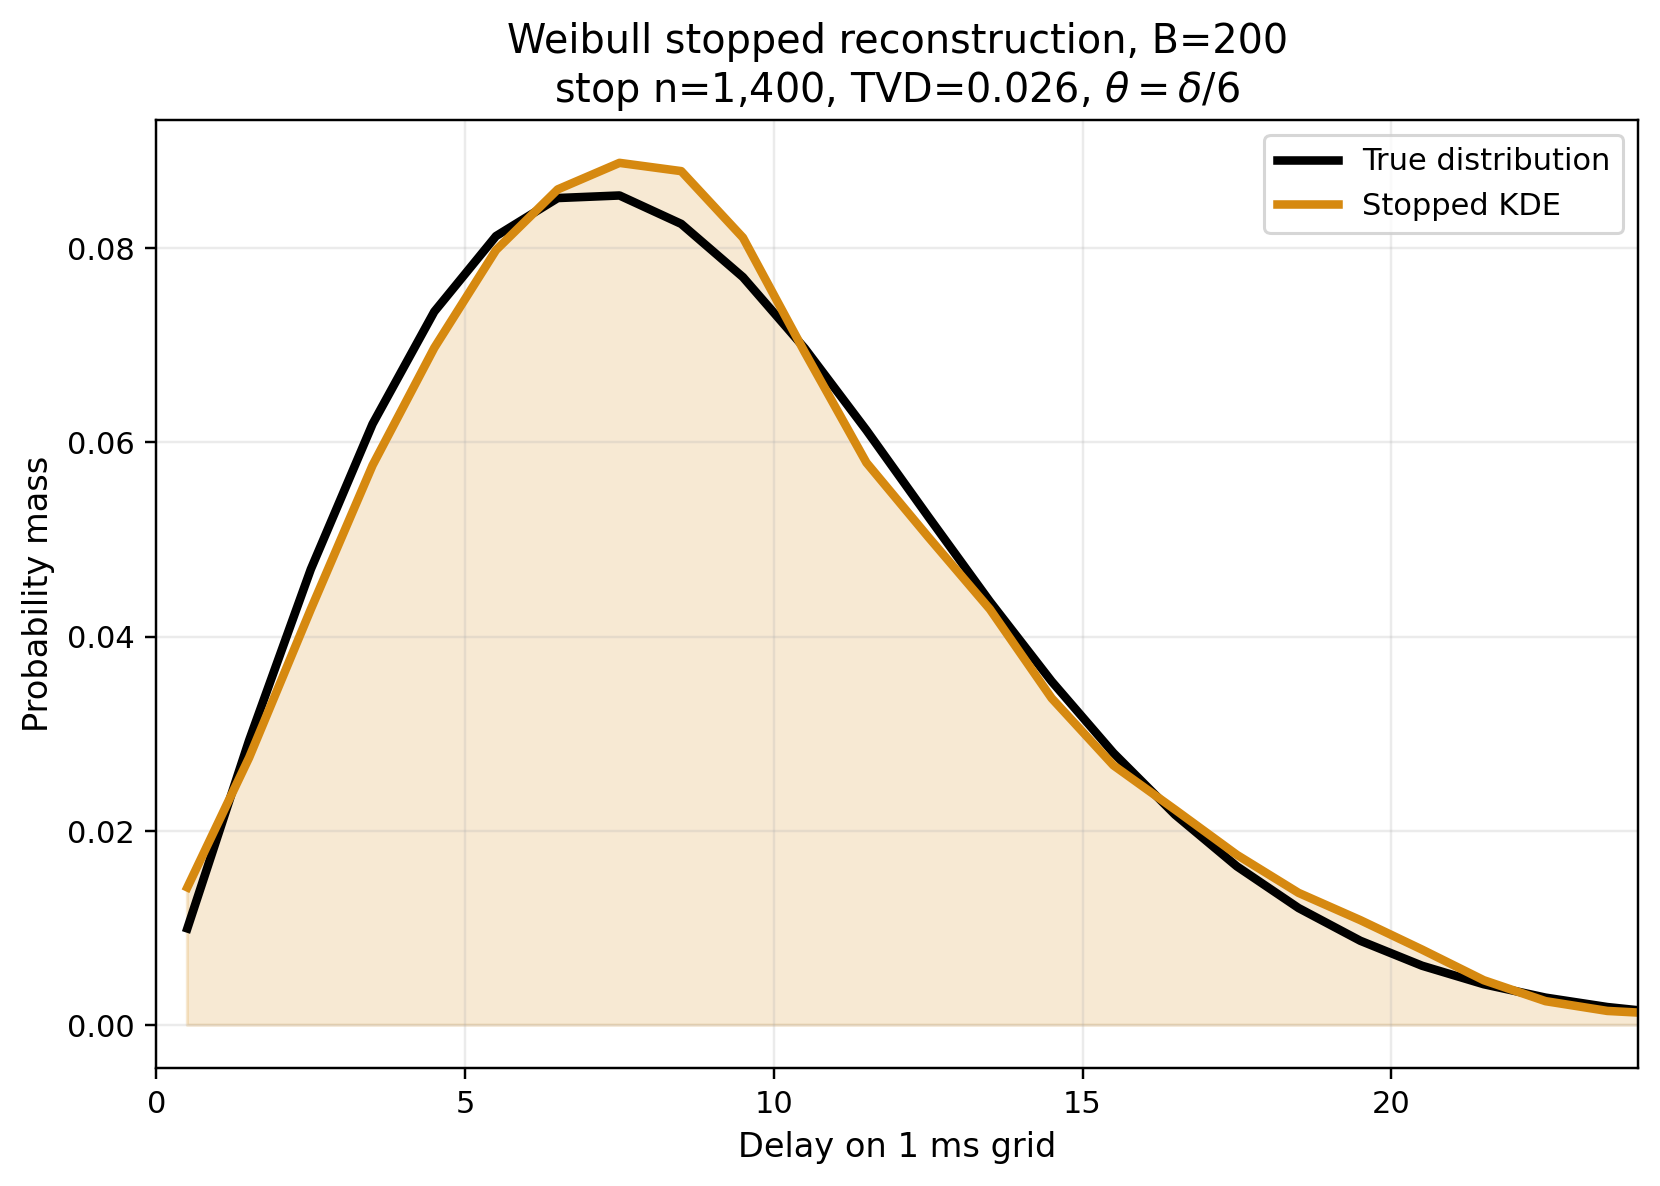
\includegraphics[width=0.92\textwidth]{stopped_distribution_weibull_b200.png}
\caption{Zoomed stopped KDE reconstruction for the Weibull distribution at \(B=200\) and \(\theta=\delta/6\). The plot shows whether the asymmetric rise, peak, and tail are preserved at the stopping time.}
\label{fig:stopped-distribution-weibull-b200}
\end{figure}

Figure \ref{fig:stopped-distribution-weibull-b200} shows what the conservative \(B=200,\theta=\delta/6\) decision means in distributional terms for the hardest continuous shape. The illustrative Weibull run stops after 1,400 packets, and TVD against truth at the stopping point is well inside the 0.05 target. The plot is more informative than the scalar value alone. It shows that the estimate preserves the steep left rise, the peak, and the longer right tail, which are exactly the features that would matter if a later capacity decision were based on distribution identity. The normal and lognormal stopped reconstructions in Appendix Figures \ref{fig:app-stopped-distribution-normal-b200} and \ref{fig:app-stopped-distribution-lognormal-b200} show the easier cases. Their centres and tails are also aligned, but they add less to the argument once the Weibull reconstruction has been inspected directly.

\begin{figure}[htbp]
\centering
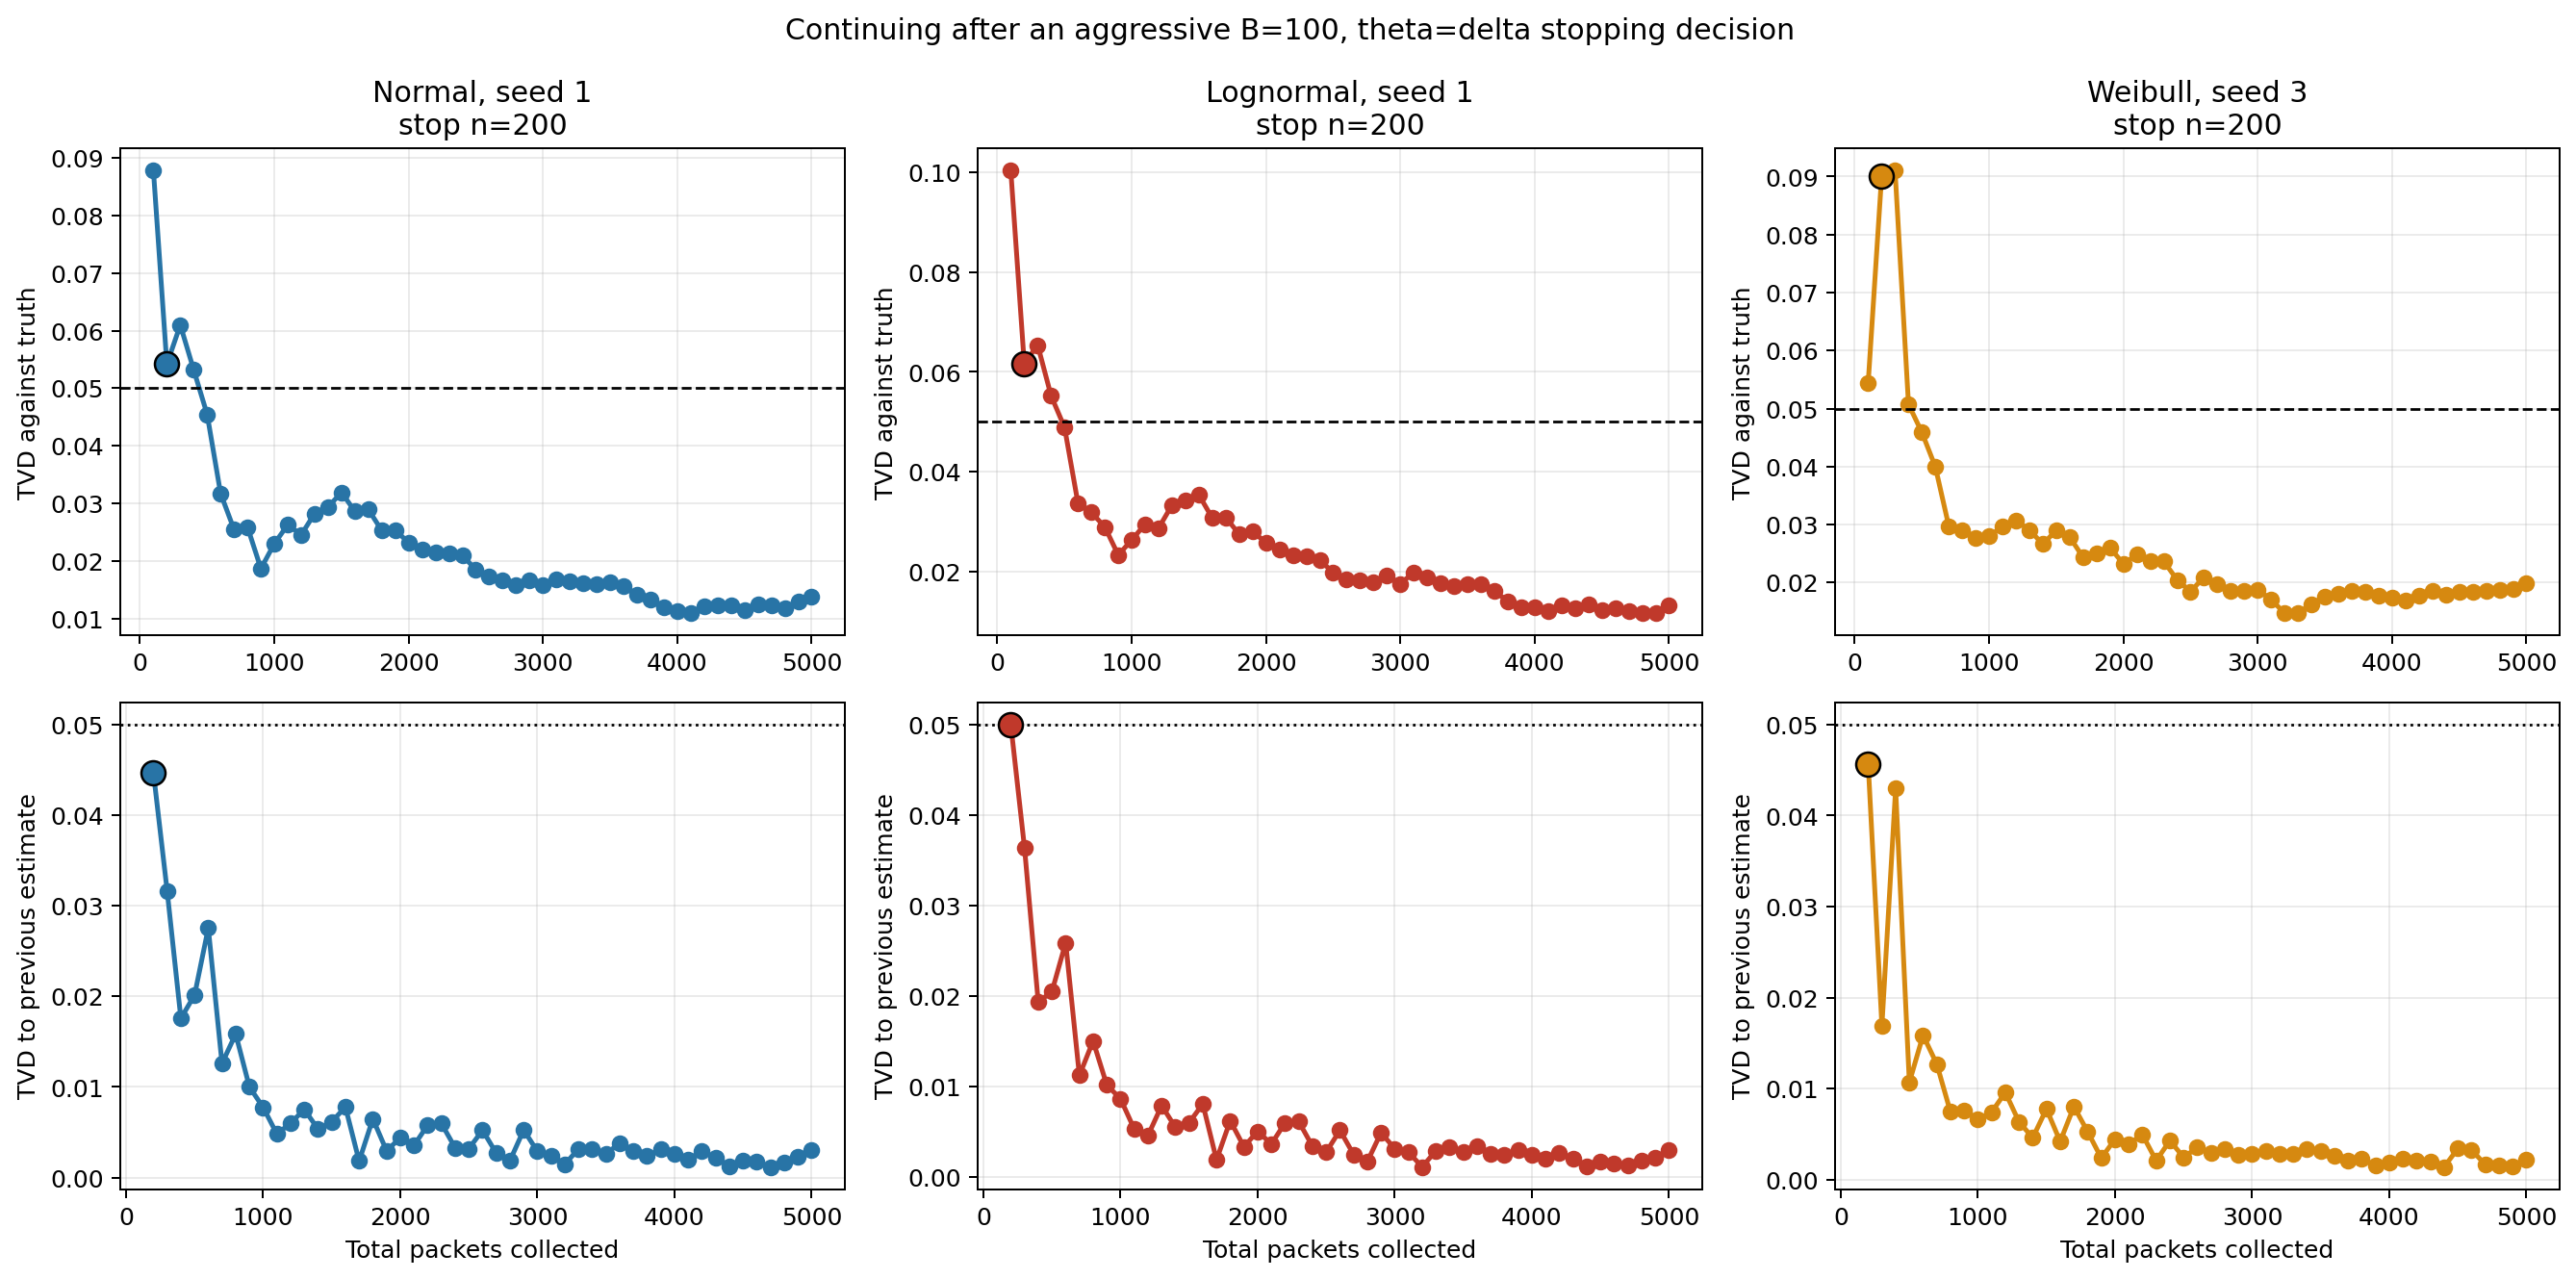
\includegraphics[width=\textwidth]{early_stop_trace_cont_all.png}
\caption{Continued traces after the aggressive \(B=100,\theta=\delta\) stopping decision. The upper row shows TVD against truth after the rule would have stopped. The lower row shows the observed TVD to the previous cumulative estimate.}
\label{fig:early-stop-trace-cont-all}
\end{figure}

Figure \ref{fig:early-stop-trace-cont-all} explains why the loose \(B=100,\theta=\delta\) rule fails. In the examples shown, the observed TVD to the previous estimate falls below the stopping threshold at 200 packets, so the rule stops. The upper row shows that true TVD is still above 0.05 at that point. Continuing the same run beyond the stopping decision shows TVD against truth falling below the target after later batches. The failure is premature conclusion: the first two cumulative reconstructions can be close to one another because both are under-sampled, not because both are correct. In a capacity-estimation setting, this would be a serious error because the system could classify a path state using a distribution that had not yet learned the relevant tail or peak. In this design, tightening \(\theta\) or increasing \(B\) reduces this false-stability event by requiring a stronger sign of convergence before stopping.

\begin{table}[htbp]
\centering
\small
\begin{tabular}{llrrrr}
\toprule
Distribution group & Configuration & First & Second & Third & Median \(n_{\mathrm{stop}}\) range \\
\midrule
Continuous & \(B=100,\theta=\delta\) & 0.53 & 0.42 & 0.49 & 200 to 200 \\
Continuous & \(B=100,\theta=\delta/6\) & 0.98 & 0.95 & 0.97 & 900 to 900 \\
Continuous & \(B=200,\theta=\delta/6\) & 1.00 & 1.00 & 0.99 & 1,400 to 1,600 \\
Discrete & \(B=100,\theta=\delta\) & 0.13 & 0.12 & 0.02 & 300 to 400 \\
Discrete & \(B=100,\theta=\delta/6\) & 0.93 & 0.95 & 0.95 & 1,300 to 1,700 \\
Discrete & \(B=300,\theta=\delta/5\) & 1.00 & 1.00 & 1.00 & 2,250 to 3,000 \\
\bottomrule
\end{tabular}
\caption{Selected adaptive stopping operating points. For the continuous group, the three correctness columns correspond to normal, lognormal, and Weibull. For the discrete group, they correspond to binomial, Zipf, and piecewise.}
\label{tab:adaptive-operating-points}
\end{table}

\section{Discrete Stopping Behaviour}

\begin{figure}[htbp]
\centering

\includegraphics[width=\textwidth]{correctness_grid_disc.png}
\caption{Correctness of adaptive stopping for the discrete distributions. The multi-modal piecewise distribution is the hardest case, and the vertical axis increases upwards with batch size.}
\label{fig:adaptive-disc-correctness}
\end{figure}

Figure \ref{fig:adaptive-disc-correctness} shows that the discrete distributions are more demanding. At \(B=100\) and \(\theta=\delta\), correctness is only 0.13 for binomial, 0.12 for Zipf, and 0.02 for the piecewise distribution. The PMF estimate can appear stable before enough mass has been allocated to each support point, especially when the distribution has several separated modes. Tightening the threshold helps, but the safest region is reached later than in the continuous case. With \(B=300\) and \(\theta=\delta/5\), all three discrete distributions reach 100 percent correctness, with median stopping times between 2,250 and 3,000 samples. Those counts remain far below the corresponding worst-case learning bounds, although the efficiency gains are naturally smaller than in the continuous KDE case because the theoretical bounds for these 20-point discrete distributions are already much lower. The discrete result reinforces the main lesson from the statistical evaluation: irregular shape, not just support size, controls how conservative the stopping rule needs to be.

Appendix \ref{app:adaptive-diagnostics} includes the corresponding total-packets plot and stopping-time TVD plot for the piecewise distribution. Those diagnostics show that the piecewise case is hard because loose thresholds and small values of \(B\) leave many stopped estimates near or above the target line. With tighter thresholds or larger values of \(B\), the stopped TVD moves safely below 0.05, often around 0.02 to 0.03, leaving useful safety margin.

\section{Implications for the use case}

The adaptive stopping evaluation gives a clear message for the stationary direct-sampling tasks tested here. A loose stability threshold is unsafe because the estimate can look locally stable before it is globally accurate. A stricter threshold, especially \(\theta=\delta/6\) or \(\theta=\delta/5\), removes most early stopping failures at a small sample cost compared with the theoretical bound. For continuous KDE reconstruction, \(B=200,\theta=\delta/6\) is the conservative operating point used to carry the method forward. For discrete PMF reconstruction, \(B=300,\theta=\delta/5\) plays the same role. These should not be read as universal recommendations. They show that the approach is feasible, but that feasibility depends on choosing a point in the correctness-efficiency trade-off that gives enough safety margin. The \(B=100\) setting remains useful as an aggressive comparison and as a failure diagnostic under loose thresholds, but the heatmaps show that the larger batch gives a cleaner reliability story across normal, lognormal, and Weibull delays.

These operating points are scoped to the experimental conditions of this section. Samples are independent and identically distributed within each run, the underlying distribution does not change during a run, and the input stream is complete and ordered. Each assumption is relaxed in the network experiments. A drifting distribution can defeat the stability check by producing small batch-to-batch changes that never accumulate, and a sudden change can defeat it by producing one large jump that reads as continued instability. The stopping rule used here is also a simple two-step comparison and does not enforce a minimum sample count. It provides no formal finite-sample guarantee beyond the empirical correctness measured in this section. A more conservative variant could require stability over several consecutive batches, or could require a minimum \(B\) before the first comparison is allowed. The stationary case does not require these extensions, although the use-case experiments keep them in view. Computational cost is dominated by per-batch reconstruction. The PMF estimator costs one increment per sample. The KDE estimator with Scott's rule costs work proportional to the number of samples times the number of grid points at evaluation time, which is the source of most per-batch cost on the 1 ms grid.

Stopping is not the final operational decision; it decides when the distribution estimate is stable enough to be trusted. The use case can then perform the identification step, comparing that stable estimate with an empirical low-load operating state rather than with a ground-truth reference distribution. Early stopping error is the risk of trusting an unstable estimate. Identification error is the risk of drawing the wrong capacity conclusion from a stable estimate. By reducing the first risk, the first two evaluations make the later capacity experiment a fairer test of whether distributional change is an informative signal for remaining path capacity.

\chapter{Single Link Capacity Response}
\label{sec:eval-capacity-use-case}

The single-link chapter is the first full use-case iteration. The previous two chapters establish the statistical machinery in isolation. Delay distributions can be reconstructed from samples, and adaptive stopping can decide when an estimate is stable without access to ground truth. The remaining question is whether a sequence of stopped distributions can support an operational judgement about remaining capacity.

The single-link experiment is a pressure test for the project logic. The initial hypothesis was that the first significant distributional change would mark the point where added traffic had consumed the useful capacity headroom. That hypothesis is plausible from a distribution-testing perspective, but it is too blunt operationally because traffic can perturb delay gradually before the path reaches a capacity-relevant boundary. The refined hypothesis is stronger: the boundary should appear as an acceleration in the distributional response, rather than as the first detectable difference.

\section{Experimental design}

The topology contains one 10 Mbit/s point-to-point link. A monitored probe flow crosses the link while a controlled User Datagram Protocol cross-traffic flow is increased additively. The configured link rate is used by the simulator to create the experimental condition, but it is not used by the monitoring decision. The monitor observes received probe delays, reconstructs a stopped delay distribution at each offered-load level, and compares distributions across load levels.

The experiment uses one hop to isolate the capacity mechanism from path composition, routing, and multi-queue effects. If the method cannot produce a meaningful signal in a single controlled link, there is little reason to expect it to work in a larger topology. If it does work, the single-hop result becomes the baseline against which the multi-hop chapter can be judged.

The final experiment uses an additive load sweep rather than the earlier bracket-refinement design described in the use case. The load ratio starts at 0.050 and increases in steps of 0.025 until 1.300 of the configured link rate. This common grid makes the TVD response visible across all seeds and delay families. It also bounds the precision of the result. A reported boundary of 0.925 means that 0.925 is the first load-grid point satisfying the criterion, not that the physical capacity boundary has been measured to three decimal places.

The delay process is drawn from the same three continuous families used earlier: normal, lognormal, and Weibull. The monitor is not told which family generated the samples. This preserves the distribution-agnostic constraint from the sample-complexity chapter and ensures that success is not due to fitting a known parametric model.

At each offered-load level \(r_i\), samples are collected until the adaptive stopping rule returns a stable estimate \(\widehat{P}_{r_i}\). The continuous stopping configuration is retained, with \(B=200\), \(\theta=\delta/6\), and \(\delta=0.05\). This choice is conservative because the capacity decision depends on comparing distributions. An unstable estimate would create a misleading capacity signal even if the later comparison rule were well chosen.

The score at load \(r_i\) is measured against the first low-load estimate \(\widehat{P}_{r_0}\):
\[
S_i =
d_{\mathrm{TV}}\left(\widehat{P}_{r_i},\widehat{P}_{r_0}\right).
\]
The low-load estimate is not treated as a known ground-truth reference distribution. It is the first empirical operating state observed by the monitor. The purpose of \(S_i\) is to measure how far the path has moved from that starting state as load increases.

Two distributional criteria are compared because each tests a different interpretation of the use case. The first is ordinary distribution change, defined as the first load for which \(S_i \geq 0.05\). This tests the initial hypothesis that any significant identity failure marks the capacity boundary. The second is TVD rate change, which detects the first sharp acceleration in \(S_i\) as load increases. Let
\[
\Delta S_i = S_i-S_{i-1}, \qquad
g_i = \max\left(0,\frac{\Delta S_i}{r_i-r_{i-1}}\right).
\]
Locally decreasing TVD is treated as zero slope so that sampling noise does not reduce the low-load baseline. Once at least two previous finite slopes are available, the baseline is
\[
m_i = \mathrm{median}\{g_j: 1 \leq j < i,\ g_j\ \mathrm{finite}\}.
\]
A load is marked as accelerated when
\[
\Delta S_i \geq 0.05
\qquad \mathrm{and} \qquad
g_i \geq 5 \cdot \max(m_i,10^{-4}).
\]
The \(10^{-4}\) lower bound prevents the median baseline from degenerating to zero when early TVD increments are numerically flat on the 0.025 load grid. These constants are empirical operating choices used to test whether the response curve has changed character, not a universal theory of congestion.

The response-rate criterion is not intended to estimate a universal congestion threshold. It is a diagnostic rule for detecting a change in the shape of the TVD response curve. The minimum jump is tied to the reconstruction target \(\delta=0.05\), so a boundary requires a distributional movement at least as large as the tolerated reconstruction error. The slope multiplier is then ablated in the results to check whether the selected boundary depends on one arbitrary acceleration constant.

The run uses 100 seeds for each delay family, giving 300 independent single-hop runs. Results are reported as a ratio of the configured link rate, which is used only for post-hoc evaluation. The simulation uses finite first-in, first-out queues, and the analysis records endpoint delivery loss as a sanity check, but loss is not used as the capacity criterion.

\section{Results}

Table \ref{tab:observable-single-methods} shows that the initial hypothesis does not survive the single-link experiment. The ordinary distribution-change rule fires in every run, but its median detection point is only 0.625 of the configured link capacity. A median of 0.625 is too early to be a defensible capacity estimate. The distribution-specific medians explain the failure: lognormal detects at 0.575, normal at 0.600, and Weibull at 0.925. The same TVD threshold is therefore measuring ordinary shape sensitivity for some delay families and a capacity-near transition for others. Appendix Figure \ref{fig:observable-single-methods} retains the corresponding summary plot.

\begin{table}[htbp]
\centering
\small
\begin{tabular}{lrrr}
\toprule
Criterion & Detected runs & Median ratio & Interquartile range \\
\midrule
First distribution change & 300 of 300 & 0.625 & 0.575 to 0.925 \\
TVD rate change & 300 of 300 & 0.925 & 0.925 to 0.925 \\
\bottomrule
\end{tabular}
\caption{Distributional capacity criteria in the single-hop 10 Mbit/s experiment. Ratios are relative to the configured link rate.}
\label{tab:observable-single-methods}
\end{table}

The TVD rate-change rule supports the refined hypothesis. It detects at 0.925 of configured capacity in all 300 single-hop runs, with an interquartile range of 0.925 to 0.925. The number must be read as a grid point from the 0.025 load sweep. The evidence lies in the same grid point being selected across the three tested normal, lognormal, and Weibull delay families, rather than in decimal precision. The response-rate criterion removes the dependence on where each distribution first crosses a fixed TVD threshold and instead detects the point where the curve changes character.

\begin{figure}[htbp]
\centering
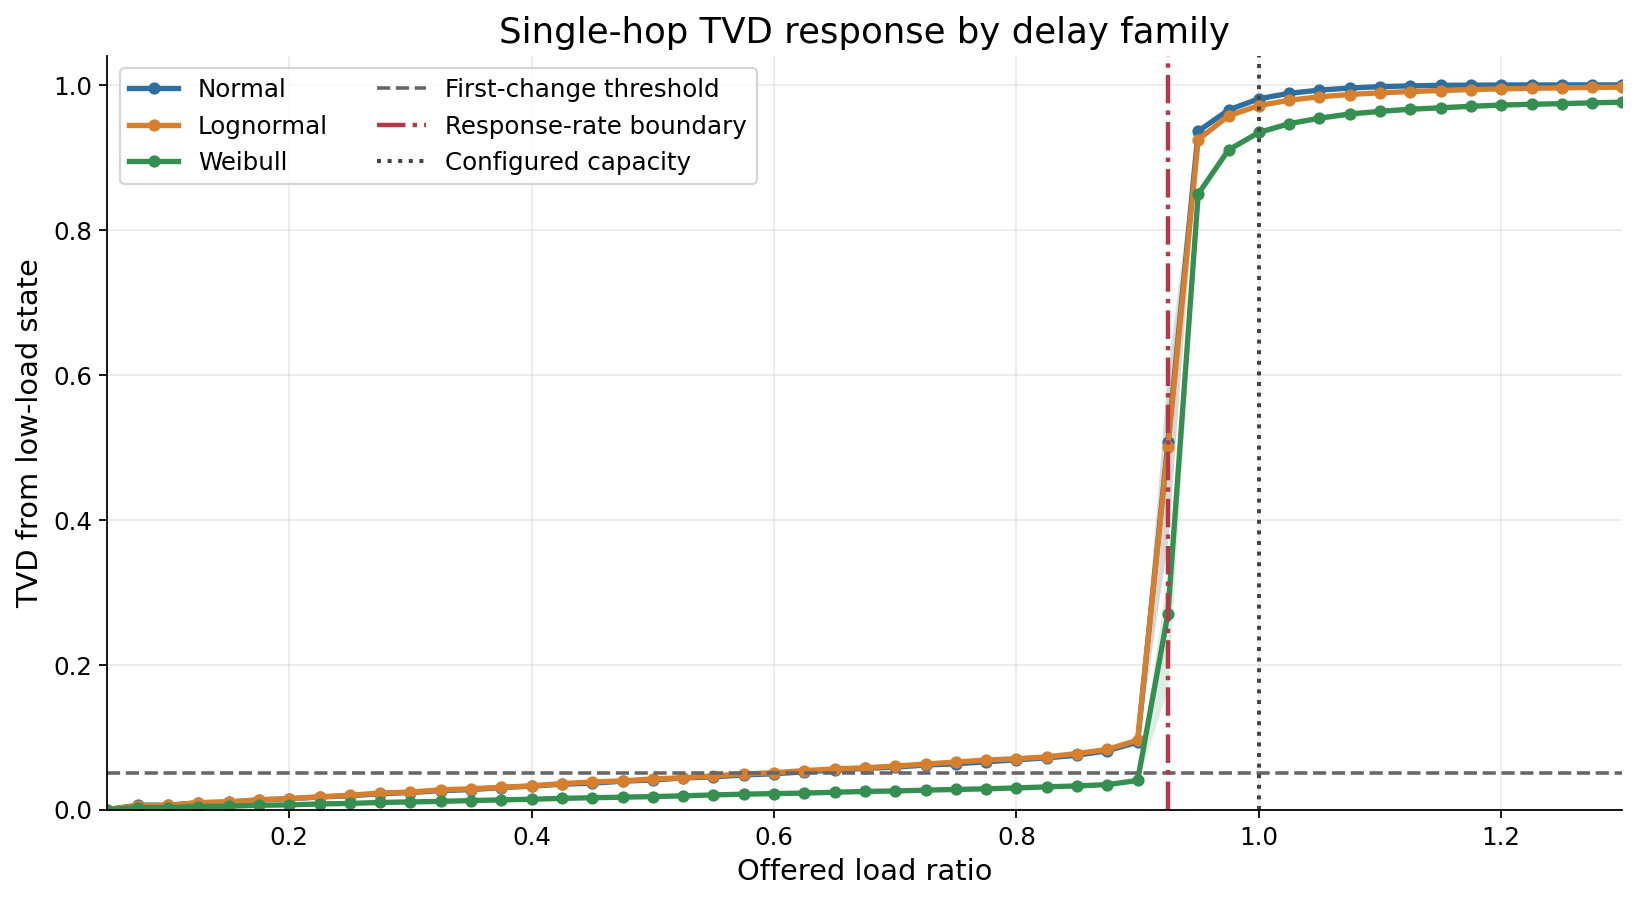
\includegraphics[width=\textwidth]{observable_capacity_single_tvd_by_distribution.png}
\caption{Single-hop TVD response by delay family. Each curve shows the median TVD from the first low-load state, with interquartile ranges across 100 seeds.}
\label{fig:observable-single-tvd-by-dist}
\end{figure}

Figure \ref{fig:observable-single-tvd-by-dist} explains the result mechanistically. Normal and lognormal delays cross the 0.05 first-change threshold gradually, long before the configured capacity. Weibull remains below the threshold for longer, which is why the first-change rule appears to work for that family in isolation. Across families, the same first-change rule reports medians of 0.575, 0.600, and 0.925. That spread indicates sensitivity to ordinary distributional drift rather than a stable capacity boundary.

The response-rate criterion instead detects the point where the TVD curve stops increasing slowly and begins increasing sharply. In Figure \ref{fig:observable-single-tvd-by-dist}, that bend occurs at 0.925 for all three delay families. The criterion uses the change in the rate of distributional movement, not the first non-zero distance from the starting state.

\begin{figure}[htbp]
\centering
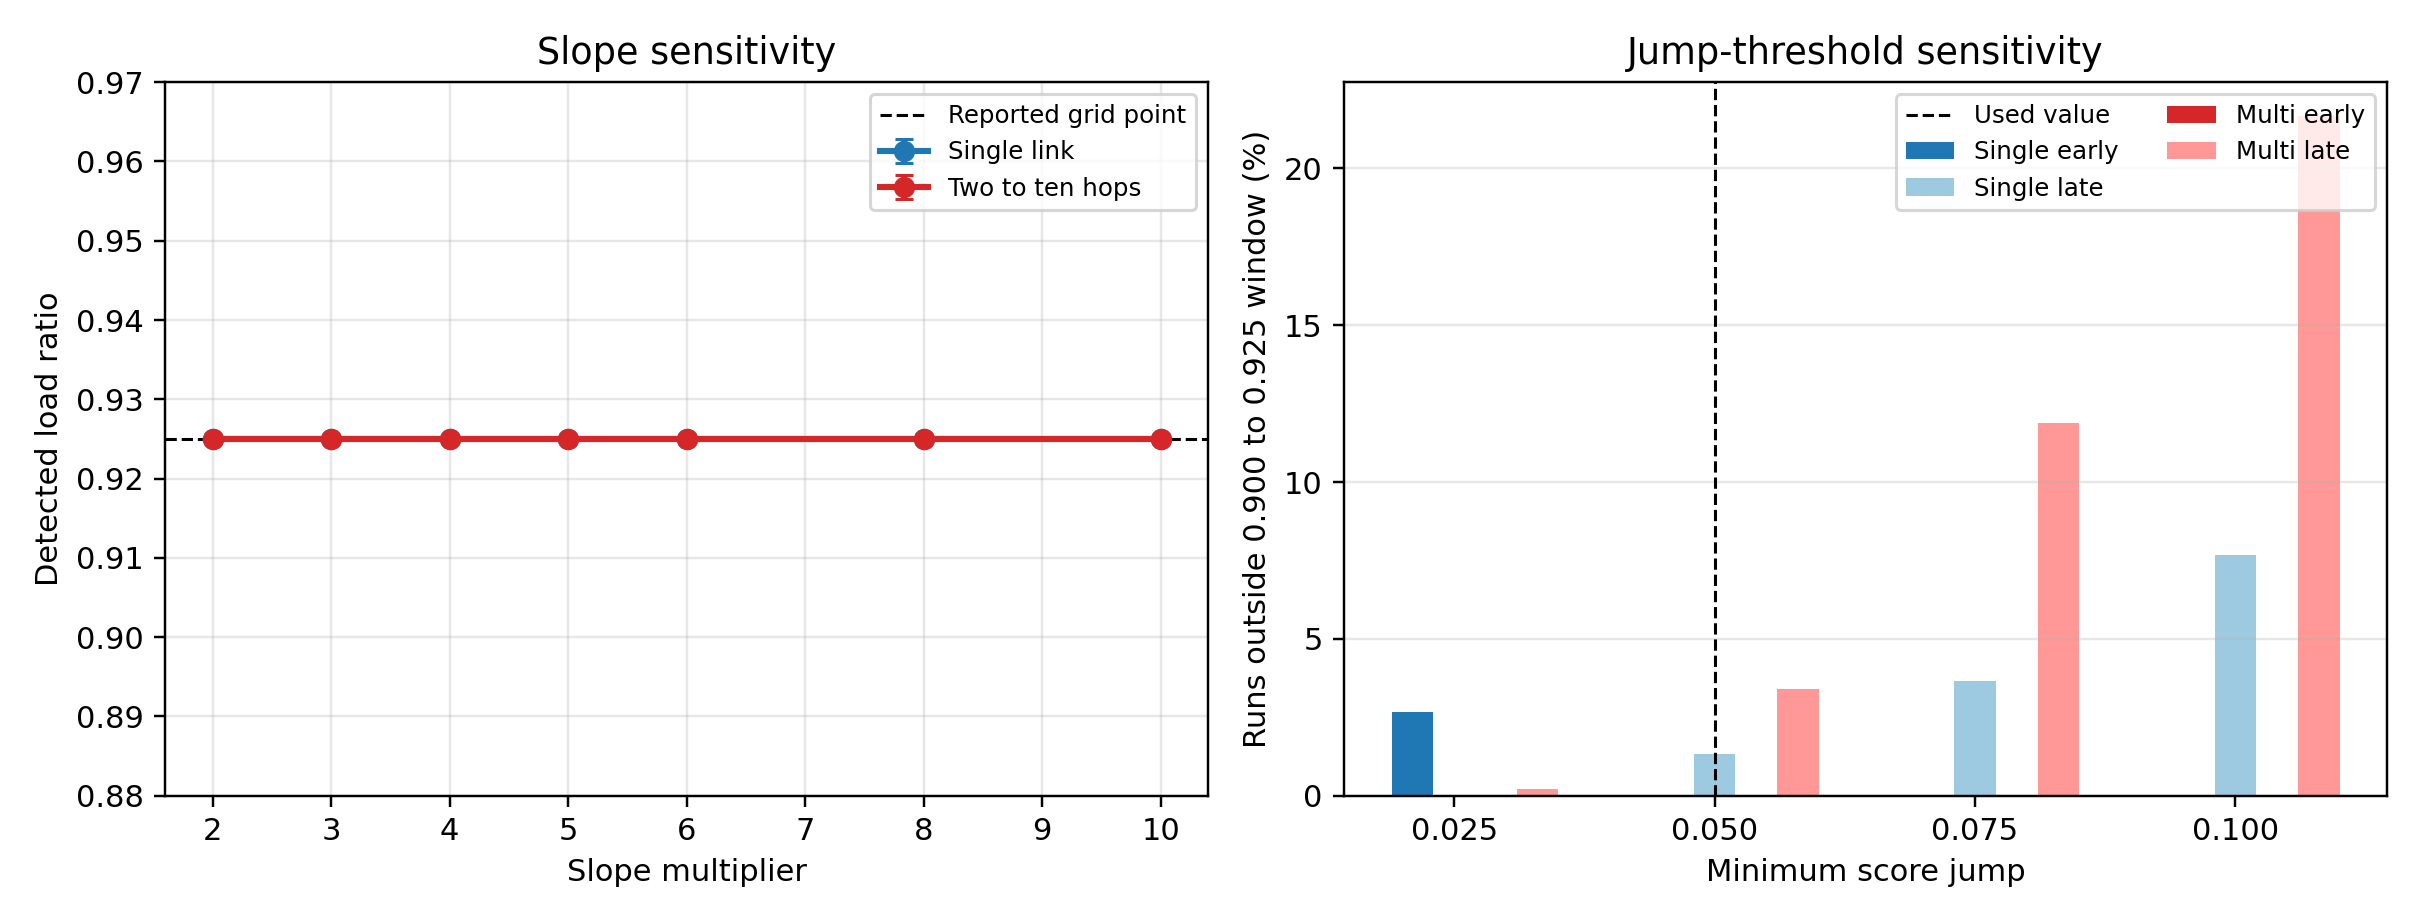
\includegraphics[width=\textwidth]{response_rate_parameter_sensitivity.png}
\caption{Sensitivity of the response-rate criterion on the saved single-link and multi-hop outputs. The median boundary remains at the 0.925 grid point for slope multipliers from 2 to 10. The minimum score jump is more consequential: values below 0.05 admit early outliers, while larger values increasingly delay some runs beyond 0.925.}
\label{fig:response-rate-sensitivity}
\end{figure}

Figure \ref{fig:response-rate-sensitivity} addresses the main free-parameter risk in the refined criterion. The five-times slope multiplier is not uniquely responsible for the 0.925 result, since multipliers from 2 to 10 give the same median and interquartile range on the saved outputs. The minimum score jump matters more. A jump threshold of 0.025 admits early detections below 0.900 in 8 of the 300 single-link runs, while 0.075 and 0.100 increasingly shift some detections to 0.950. The chosen value of 0.05 is therefore best described as a conservative empirical operating point aligned with the reconstruction TVD target. It is not a theorem, and it should be ablated again if the load grid, queue size, or traffic model changes.

A simple scalar comparator was also run on the same stopped samples. Mean, median, 95th percentile, and 99th percentile delay were each compared with their first low-load value, and the first load with at least a 5 percent relative change was recorded. Table \ref{tab:single-scalar-baselines} includes the TVD response-rate row on the same reporting scale. Scalar thresholds match the 0.925 median in this controlled setting, yet introduce early and late outliers that the TVD response-rate criterion does not. The 99th percentile baseline fires as early as 0.075 in some runs, while median delay fires as early as 0.550. The measured advantage here is the absence of early and late detections under one fixed rule, not a different median boundary.

\begin{table}[htbp]
\centering
\small
\begin{tabular}{lrrrr}
\toprule
Signal & Detected runs & Median ratio & Early rate below 0.900 & Late rate above 0.925 \\
\midrule
TVD response rate & 300 & 0.925 & 0.000 & 0.000 \\
Mean delay & 300 & 0.925 & 0.003 & 0.077 \\
Median delay & 300 & 0.925 & 0.023 & 0.073 \\
95th percentile delay & 300 & 0.925 & 0.013 & 0.063 \\
99th percentile delay & 300 & 0.925 & 0.020 & 0.070 \\
\bottomrule
\end{tabular}
\caption{Distributional and scalar baselines on the single-link outputs. Scalar delay rows use a 5 percent relative first-change threshold against the first low-load value.}
\label{tab:single-scalar-baselines}
\end{table}

Endpoint delivery loss provides a useful sanity check on the interpretation, although it is not the proposed detection method. In the same single-link outputs, the TVD response-rate boundary appears at 0.925 in all 300 runs, while endpoint cross-traffic loss first appears at 0.950 and the sparse probe stream does not show loss. Since the load grid has 0.025 spacing, this is the smallest non-zero gap the experiment can resolve. The comparison is therefore a resolution-limited timing result, not a broad claim that distributional monitoring always dominates loss counting.

\begin{table}[htbp]
\centering
\small
\begin{tabular}{p{0.26\textwidth}p{0.24\textwidth}p{0.39\textwidth}}
\toprule
Signal & First observed load ratio & Interpretation \\
\midrule
TVD response rate & 0.925 in all 300 runs & Distributional boundary under the tested criterion \\
Endpoint cross-traffic loss & 0.950 & First delivery-failure signal, one grid step later \\
Probe packet loss & Not observed & Too sparse to act as the trigger in these runs \\
\bottomrule
\end{tabular}
\caption{Single-link sanity check comparing the distributional boundary with endpoint delivery loss. Loss is reported only to contextualise the timing of the proposed signal.}
\label{tab:single-loss-sanity}
\end{table}

\section{Bursty cross traffic}

The constant-rate experiment gives a clean first test, but it is also a favourable traffic model. A second single-link stress test replaces the constant cross-traffic source with Pareto on-off User Datagram Protocol traffic. The on and off periods both use a bounded Pareto random variable with scale 0.02, shape 1.5, and bound 0.5 seconds. During on periods, the sender transmits at twice the swept average rate, so an average offered load near 0.5 already contains on-period bursts close to the nominal link rate. The same adaptive stopping rule and response-rate criterion are used without re-tuning.

\begin{table}[htbp]
\centering
\small
\begin{tabular}{lrrr}
\toprule
Signal & Detected runs & Median ratio & Interquartile range \\
\midrule
First distribution change & 300 of 300 & 0.475 & 0.475 to 0.475 \\
TVD rate change & 290 of 300 & 0.475 & 0.475 to 0.500 \\
Endpoint cross-traffic loss & 300 of 300 & 0.575 & 0.550 to 0.600 \\
Probe packet loss & 0 of 300 & Not observed & Not observed \\
\bottomrule
\end{tabular}
\caption{Bursty single-link stress test over normal, lognormal, and Weibull delay families with 100 seeds each. Loss remains a sanity check rather than a capacity criterion.}
\label{tab:observable-bursty-methods}
\end{table}

Table \ref{tab:observable-bursty-methods} changes the interpretation of the boundary. The median TVD rate-change point is 0.475 of the average offered load, not 0.925. At a swept average load of 0.475, the on-period traffic rate is 0.950 of the link rate. The shift is therefore a consequence of the traffic construction rather than a contradiction of the constant-rate result. The distributional response is tracking burst pressure on the queue, not only the long-run average sending rate. Appendix Figure \ref{fig:observable-bursty-methods} keeps the summary plot for the bursty comparison, while the main text retains the Weibull response curve because it shows the incomplete 90 of 100 detection case directly.

\begin{figure}[htbp]
\centering
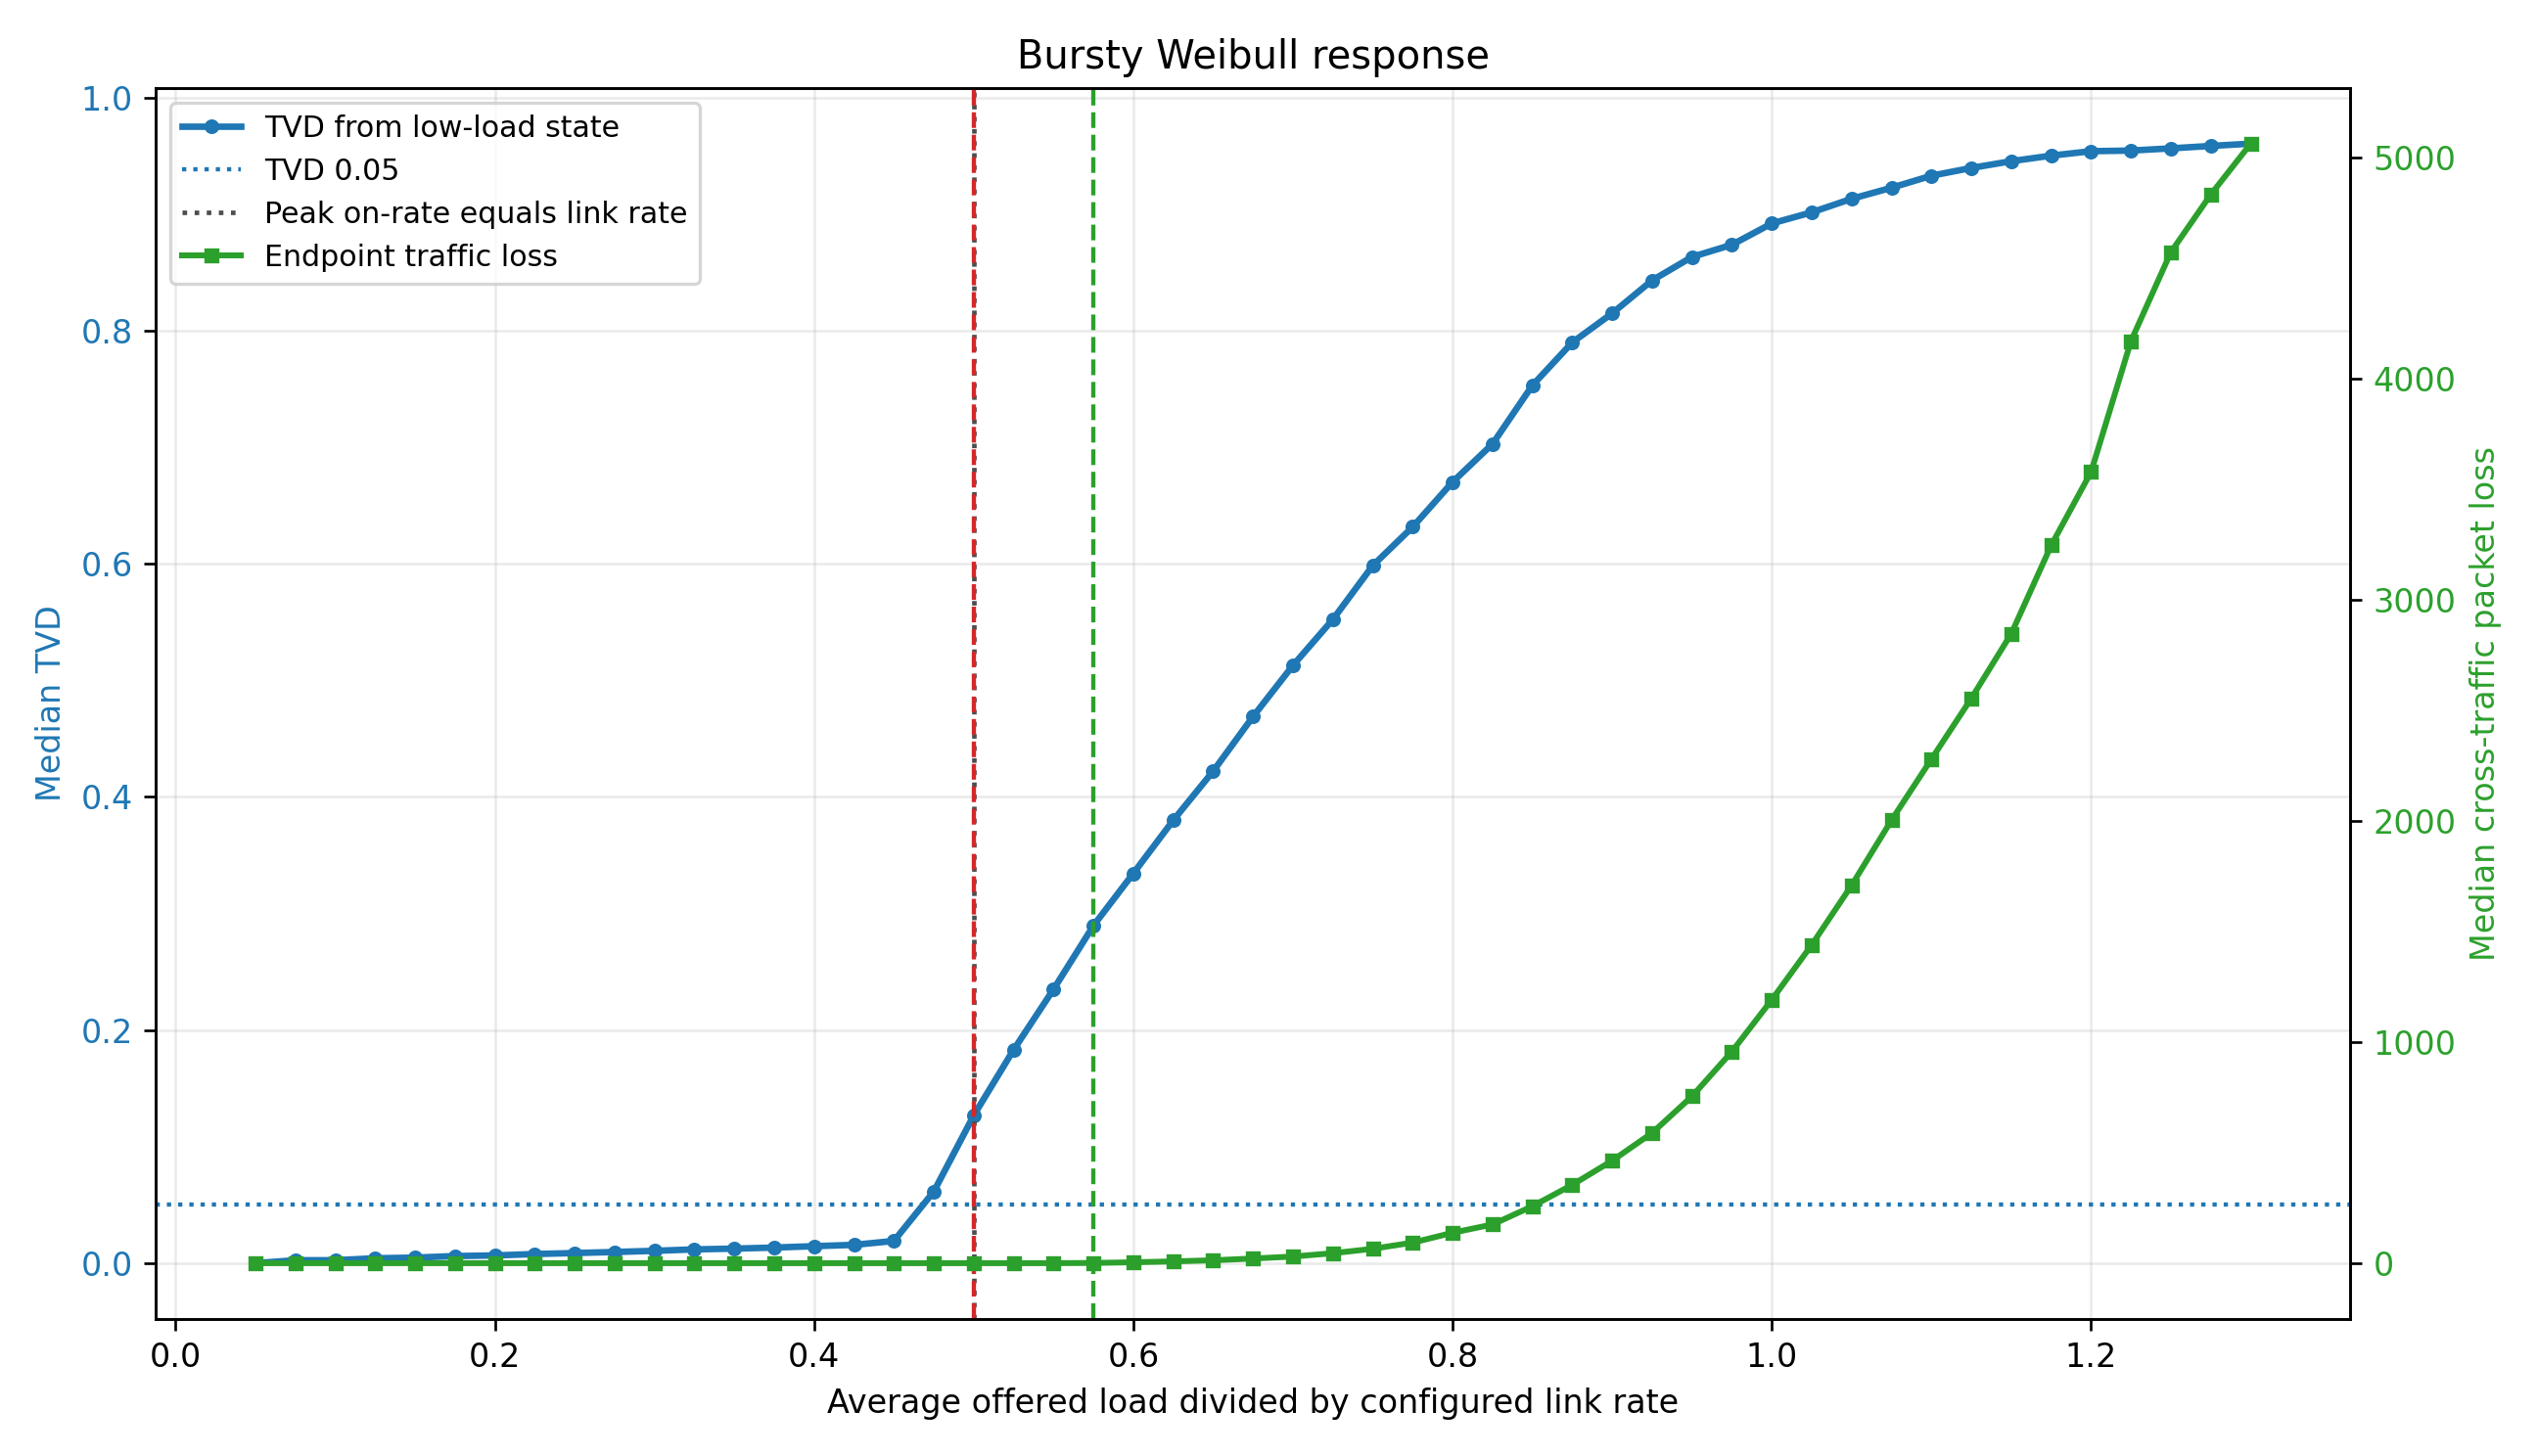
\includegraphics[width=\textwidth]{observable_capacity_bursty_tvd_loss_weibull.png}
\caption{Weibull bursty cross-traffic response. The TVD bend appears before endpoint cross-traffic loss, but the response is less complete than in the constant-rate experiment.}
\label{fig:observable-bursty-weibull}
\end{figure}

The Weibull case in Figure \ref{fig:observable-bursty-weibull} is the harder bursty setting. TVD rate change fires in 90 of 100 Weibull runs, compared with 100 of 100 normal and lognormal runs. Endpoint cross-traffic loss appears later, at a median average load of 0.575, and probe loss is still absent. The 90 percent Weibull detection rate shows that the signal is not tied to constant-rate traffic, although it is weaker than the 100 percent detection rate in the constant-rate experiment. The detected boundary should therefore be reported in terms of the offered traffic process, not only as a fraction of nominal link rate.

\section{Interpretation}

Under constant-rate traffic, defining the capacity signal as first distributional change gives a family-dependent answer. Defining it as slope acceleration gives a consistent grid point under the three tested delay families. Under bursty traffic, the same criterion moves to a lower average offered load because the queue is stressed by on-period bursts rather than by the average alone. These results revise the original operational criterion rather than proving exact physical capacity. The monitor should not ask only whether the path differs from the first state, because some difference is expected as load grows. It should ask whether the rate of difference has changed enough to indicate a new operating regime.

The single-link result carries TVD response rate forward as the main capacity signal. The claim is bounded to this controlled topology and load grid: 0.925 is the first satisfying load-grid point under constant-rate traffic, not a universal constant or an exact measurement of the physical link rate. The bursty stress test adds a second constraint on the interpretation: the detected boundary depends on the traffic process used to increase pressure. The multi-hop chapter tests whether the same criterion remains useful when the receiver observes a longer path-level delay distribution.

The repeated 0.925 value should therefore be interpreted as consistency under a shared experimental mechanism, not as evidence of a universal 92.5 percent capacity threshold. The grid, queue model, traffic pattern, and fixed decision rule all shape the reported number.

\chapter{Multi Hop Capacity Response}
\label{sec:eval-multi-hop}

The multi-hop experiment tests whether the single-link conclusion is robust or merely a clean-topology artefact. A path-level monitor does not see where along the path a delay contribution was introduced. It only sees the final packet-delay samples at the receiver. As the path grows, several links can contribute propagation, transmission, queueing, and scheduling effects to the same observed distribution.

The hypothesis at this stage is more specific than in the single-link chapter. If the signal is only absolute distributional change, then longer paths should make the method worse because more components can perturb the end-to-end delay distribution. If the signal is response acceleration, then the method should be more stable: ordinary drift may begin earlier, but the capacity-relevant bend should remain identifiable relative to the curve's own low-load trend.

\section{Experimental design}

The topology is extended to paths of two to ten point-to-point links. Each link has the same 10 Mbit/s configured rate. Cross traffic is path-wide: it enters at the first node and exits at the final node, so every link on the monitored route carries the increased load. The experiment does not try to locate a single bottleneck link. It tests whether a path-level distributional signal remains useful when traffic pressure is increased throughout the monitored path. The result is therefore a depth-invariance test under uniform load, not a heterogeneous multi-bottleneck experiment. If the response-rate criterion drifted even under uniform pressure, it would be unlikely to remain useful in less controlled topologies.

The monitoring procedure is unchanged from the single-hop chapter. At each offered-load level, the monitor collects received probe delays until adaptive stopping returns \(\widehat{P}_{r_i}\). It then computes \(S_i=d_{\mathrm{TV}}(\widehat{P}_{r_i},\widehat{P}_{r_0})\) and applies the same first-change and TVD rate-change criteria. No threshold is re-tuned for hop count. A result that required a new threshold for every path length would be much weaker operationally. The sweep uses 0.05 load-ratio spacing over most of the range, with additional 0.025-spaced points around 0.900 to 1.050. The reported multi-hop boundary is therefore also a grid point. The experiment repeats the normal, lognormal, and Weibull delay families over 100 seeds for each hop count, giving 2,700 multi-hop runs.

\section{Results}

Figure \ref{fig:observable-multi-methods} shows that the first part of the hypothesis is correct. The naive distribution-change rule becomes less useful as the path grows. Its median detection ratio is 0.25 for two hops, 0.15 for three hops, and 0.10 from four hops onwards. This behaviour is not a capacity estimate. It is the accumulation of ordinary end-to-end distributional movement across a longer path.

\begin{figure}[htbp]
\centering
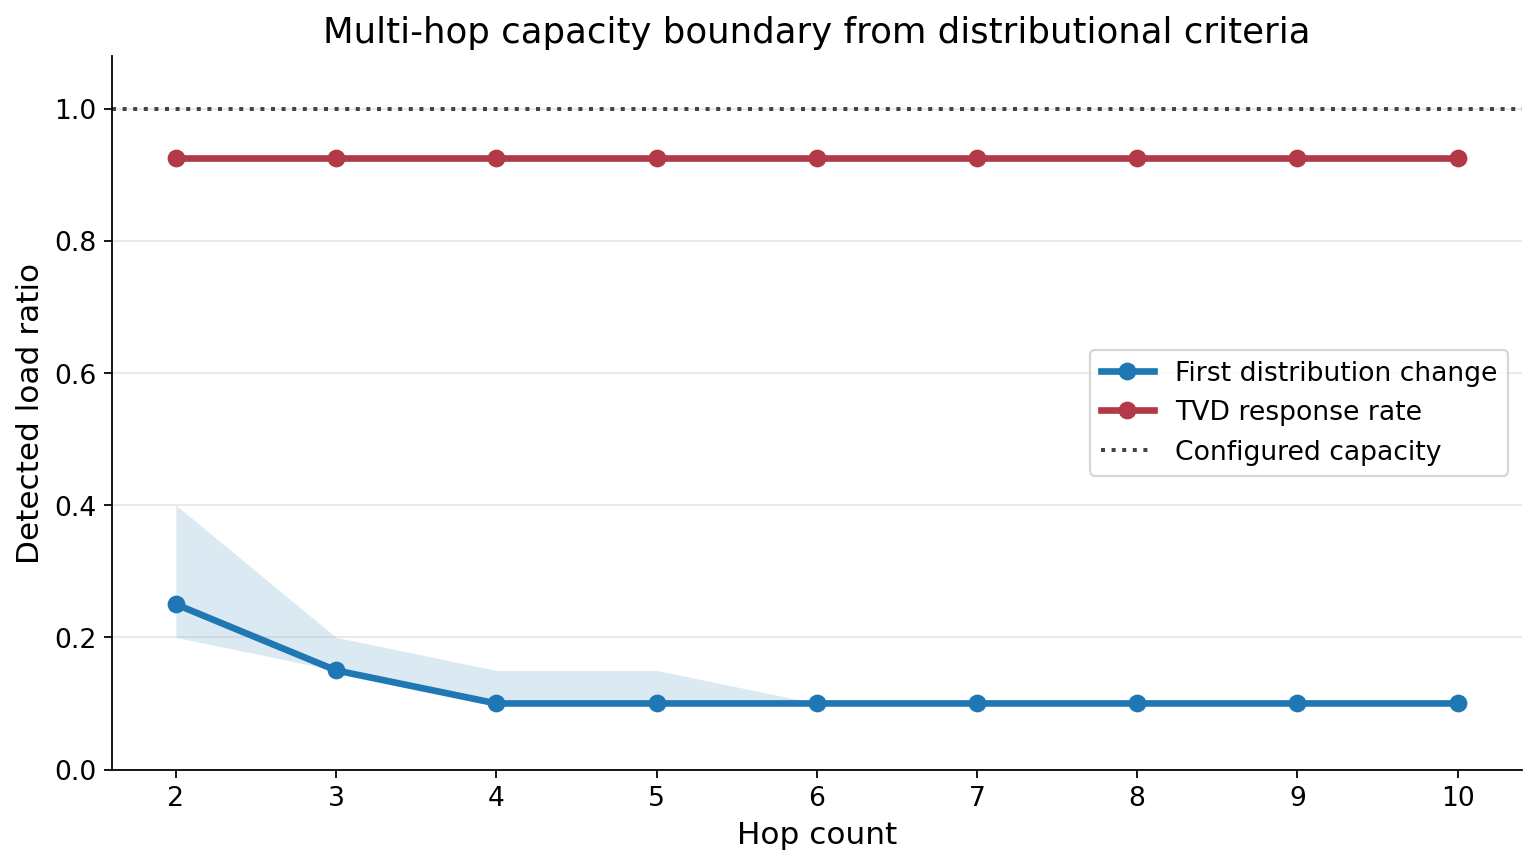
\includegraphics[width=\textwidth]{observable_capacity_multi_methods.png}
\caption{Multi-hop detection load for the two distributional capacity criteria over path-wide cross traffic.}
\label{fig:observable-multi-methods}
\end{figure}

The TVD rate-change rule remains stable across the deeper path setting. For every hop count from two to ten, and across all 2,700 multi-hop runs, the median detection ratio is 0.925 with an interquartile range of 0.925 to 0.925. As in the single-link chapter, this is a statement about the first satisfying load-grid point. Appendix Figure \ref{fig:app-observable-multi-tvd-response} shows the ten-hop response curve: TVD from the low-load baseline drifts upward well before capacity, then accelerates sharply near 0.925.

\begin{figure}[htbp]
\centering
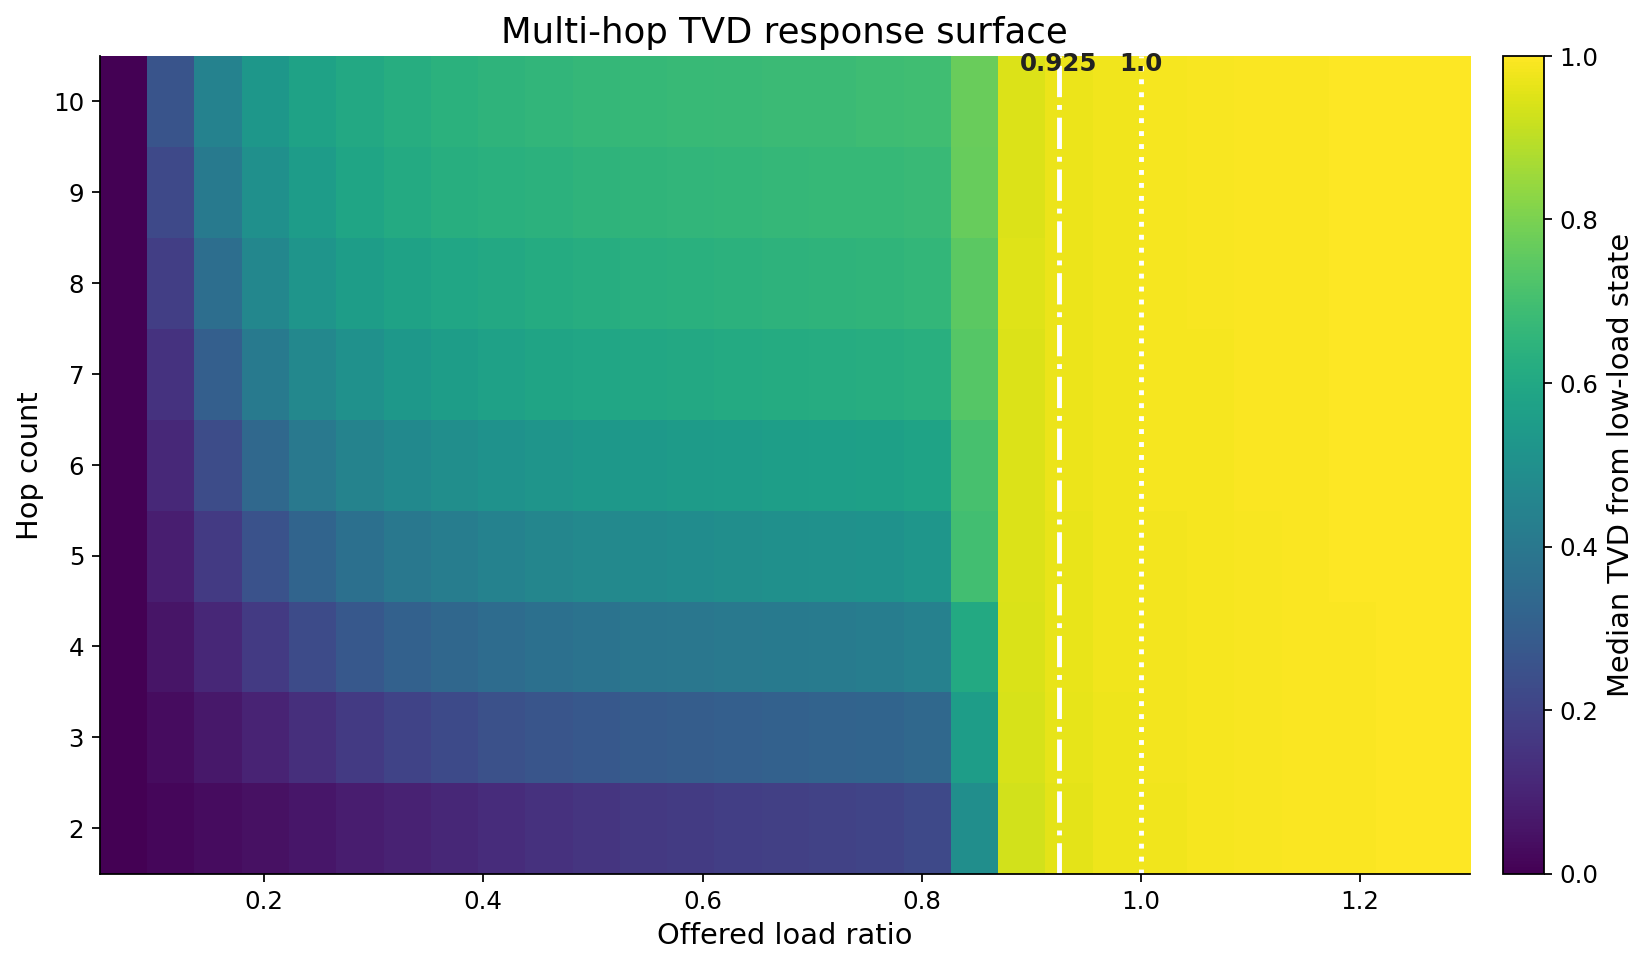
\includegraphics[width=\textwidth]{observable_capacity_multi_tvd_heatmap.png}
\caption{Multi-hop TVD response surface over offered load and hop count. The vertical line at 0.925 marks the response-rate boundary found without re-tuning by hop count.}
\label{fig:observable-multi-tvd-heatmap}
\end{figure}

Figure \ref{fig:observable-multi-tvd-heatmap} shows why the multi-hop experiment is a useful extension of the single-link experiment, while also showing its scope. As the path length grows, the end-to-end distribution is already far from the low-load state at relatively small offered-load ratios. This makes first-change detection easier in the wrong sense: the monitor can detect that the path has changed, but that fact no longer carries a useful capacity interpretation. Across hop counts, the strongest change in the TVD surface appears near the same load ratio, producing the stable response-rate boundary at 0.925.

The mechanism is visible in the heatmap. Under uniform load on identical links, each hop contributes a similar delay component, so increasing the hop count raises the absolute TVD from the low-load state. This explains why first-change detection moves earlier with path length. The response-rate rule normalises against the previous low-load slope, so gradual depth-related drift contributes to the baseline \(m_i\), while the saturation region appears as a sharp increase in \(g_i/m_i\). Since all links have the same rate and carry the same offered load, the bend occurs at approximately the same load ratio for every tested hop count.

\section{Heterogeneous slow link}

The uniform-depth experiment does not test whether the response-rate boundary survives a slow link in different path positions. A follow-up stress test therefore uses a five-hop path with one 10 Mbit/s link and four 20 Mbit/s links. The slow link is placed at the first, middle, and final hop in separate runs. Cross traffic remains path-wide, so the experiment still increases pressure across the monitored route rather than injecting traffic at one isolated link. The monitor is unchanged and does not receive the slow-link position.

\begin{table}[htbp]
\centering
\small
\begin{tabular}{lrrrr}
\toprule
Slow-link position & First-change median & First-change range & TVD rate median & Loss median \\
\midrule
First hop & 0.150 & 0.125 to 0.225 & 0.925 & 0.950 \\
Middle hop & 0.150 & 0.125 to 0.225 & 0.925 & 0.950 \\
Final hop & 0.150 & 0.125 to 0.200 & 0.925 & 0.950 \\
\bottomrule
\end{tabular}
\caption{Heterogeneous five-hop results over normal, lognormal, and Weibull delay families with 100 seeds each per slow-link position. The range column reports the interquartile range. The TVD rate-change criterion detects in all 900 runs, with interquartile range 0.925 to 0.925 in every position.}
\label{tab:observable-heterogeneous-methods}
\end{table}

Table \ref{tab:observable-heterogeneous-methods} gives a stronger multi-hop check than the uniform-depth run. First-change detection again fires early, with median 0.150 in all three slow-link positions. TVD rate change selects the 0.925 grid point in all 900 heterogeneous runs, and endpoint cross-traffic loss appears at 0.950. The slow-link position therefore does not change the response-rate boundary in this controlled path-wide setup. The experiment does not cover multiple bottlenecks or cross traffic entering and leaving at intermediate nodes. It removes the narrower concern that the previous multi-hop result only held because all links had identical configured rates. Appendix Figure \ref{fig:observable-heterogeneous-methods} contains the equivalent summary plot.

\section{Interpretation}

In longer paths, detecting any change becomes too easy and therefore uninformative. Detecting when the response changes character is more stable: TVD rate change selects the 0.925 load-grid point while using the same decision rule across all tested path lengths. The heterogeneous slow-link check extends this conclusion to a controlled non-uniform path, where the same response appears whether the slow link is first, middle, or final.

The boundary is best described as a distributional capacity boundary, not an exact physical link-rate measurement. It is the offered load at which the observed delay distribution stops changing gradually and begins changing rapidly relative to the low-load trend. This avoids claiming access to queue internals or exact physical capacity, while still capturing the operational value of finding a repeatable transition using only received delay samples.

The main depth experiment keeps every link at the same rate, and the heterogeneous stress test changes only one link at a time while preserving path-wide cross traffic. The chapter therefore does not prove robustness to intermediate cross-traffic entry and exit points, several independent bottlenecks, or route changes. The heatmap shows that longer homogeneous paths accumulate distributional distance even when they are far below the response-rate boundary. A deployment would need to distinguish ordinary path-length sensitivity from harmful capacity pressure. The response-rate rule is a first answer to that problem because it compares the curve with its own low-load trend. It is not yet a complete operational policy. A real system would still need safeguards for non-stationary traffic, route changes, and measurement gaps. Within the controlled experiment, however, the same refinement that fixed the single-link failure survives both the multi-hop depth extension and the slow-link position check.

The multi-hop path still has one end-to-end route, so the observed distribution is a lengthened version of a single path response. A multi-path setting is harder because the receiver may observe a mixture of route behaviours. The evidence here justifies carrying forward the response-rate criterion, but it also narrows the question for the next stage. The issue is no longer whether the first change is useful. It is whether a response-rate boundary remains interpretable when several path components can shape the same empirical distribution.

\chapter{Modal Analysis of Constructed Multi Path Mixtures}
\label{sec:eval-multi-path}

The multi-hop chapter keeps one route between source and destination. A multi-path setting is different. The receiver may observe packets that have crossed several route components, each with its own delay profile. The resulting empirical distribution is not simply a longer version of a single path distribution. It can become a mixture, and if the path components are sufficiently separated in delay, that mixture can become bimodal or multi-modal.

This chapter does not evaluate routed equal-cost multi-path forwarding. It isolates a narrower statistical question: if receiver-side delay samples are already a separable mixture of route behaviours, can the capacity response be associated with the changing component rather than the whole mixture? That framing keeps the experiment honest. The chapter is a modal decomposition test, not a full network-routing study.

This changes the capacity question. Applying the single-path TVD score to the whole mixture can hide which component has changed. A lightly used longer path may contribute only a small share of packets, so its capacity response can be diluted by a stable shorter path. Conversely, if most packets take the stressed path, the whole-mixture score can move early because the mixture composition dominates the comparison. The hypothesis in this chapter is therefore that multi-path capacity association should first identify modal components in the receiver-side distribution and then apply the response-rate criterion to the component that changes.

\section{Statistical basis}

Multimodality is a standard statistical signal that a sample may contain more than one generating regime. Hartigan and Hartigan's dip test formalises unimodality testing by measuring how far the empirical distribution function is from the closest unimodal distribution \cite{hartiganDip}. Silverman's test uses kernel density estimates to investigate the number of modes in a population \cite{silvermanModes}. These tests are relevant because the multi-path problem concerns both path change and the presence of several path behaviours in the same receiver-side sample.

Networking work gives the same intuition from a measurement perspective. Passive delay measurements have been used to detect multipath routing through hypothesis tests on delay observations, motivated by the fact that different paths can induce distinct delay behaviour \cite{panMultipathDelay}. Capacity-measurement work has also noted that packet-dispersion estimates can follow complicated multi-modal distributions under heavy load, and that local modes can contain useful capacity information \cite{linLmsa}. This chapter follows that line of reasoning, but does not use a formal dip-test or Silverman-test decision. The experiment uses a simpler operational decomposition: estimate the low-load mixture with the same KDE grid as earlier chapters, identify local maxima above 1 percent of the maximum density with at least eight bins of separation, take the two highest peaks, split at the lowest valley between them, and require the valley height to be no more than 80 percent of the smaller peak. Components that fail this validity check are not used for component-level capacity detection.

Let \(\widehat{P}_{r_0}^{(L)}\) denote the low-load distribution of the lower-delay path and \(\widehat{P}_{r}^{(U)}\) denote the distribution of the upper-delay path at load \(r\). The observed mixture is constructed as
\[
\widehat{M}_{r,\alpha}(x)
= (1-\alpha)\widehat{P}_{r_0}^{(L)}(x)
+ \alpha \widehat{P}_{r}^{(U)}(x-\tau),
\]
where \(\alpha\) is the traffic share on the upper-delay path and \(\tau\) is the path-delay offset. If the low-load mixture has two modes at \(m_1\) and \(m_2\), the split point is
\[
v = \arg\min_{x \in [m_1,m_2]}\widehat{M}_{r_0,\alpha}(x).
\]
The component distributions are then obtained by conditioning on \(x \leq v\) and \(x>v\). The same TVD response-rate criterion from Chapters 5 and 6 is applied to the whole mixture, the lower component, and the upper component. This non-parametric version of modal analysis avoids assuming a Gaussian mixture model, but it only works cleanly when the modes are sufficiently separated.

\section{Experimental design}

The experiment reuses the stopped NS-3 distributions from the single-link capacity runs. It is an explicit modal-mixture experiment rather than a full routed equal-cost multi-path simulation. One component remains at the first low-load distribution. The second component is shifted by 30 milliseconds to represent a higher-delay route and is swept through the same offered-load grid as the single-link experiment. The receiver sees only the weighted mixture, not the component labels. By construction, the upper component carries the single-link capacity response; the evaluation question is whether the modal decomposition can recover and associate that response after the two components have been mixed.

Four traffic splits are tested: \(\alpha=0.10,0.25,0.50,0.75\). The smallest split tests whether a stressed path can still be found when it contributes only 10 percent of observed packets. The largest split tests whether the whole mixture becomes too sensitive when most packets take the stressed component. Normal, lognormal, and Weibull delay families are each evaluated over 100 seeds, giving 1,200 multi-path mixture cases before expanding across the load grid. The link capacity used to generate the upper component is still hidden from the monitor and used only for scoring.

The design follows directly from the previous chapters. The statistical and adaptive-stopping blocks are unchanged. The new difficulty is mixture interpretation. If the whole-mixture response remains reliable across traffic splits, then modal decomposition is unnecessary. If it fails at low or high shares, then the receiver-side distribution must be interpreted as a composition of path behaviours before a capacity boundary can be associated with one route component.

\section{Results}

Figure \ref{fig:multipath-bimodal-example} shows the basic mixture structure for the Weibull case at an even traffic split. At low load, the receiver distribution has two clear modes. The dashed vertical line marks the valley used to separate the lower-delay and upper-delay components. As the upper path approaches and then exceeds the capacity boundary, the upper mode moves and broadens while the lower mode remains fixed. Whole-distribution comparison records that the receiver distribution has changed, but the modal split records which part of it changed.

\begin{figure}[htbp]
\centering
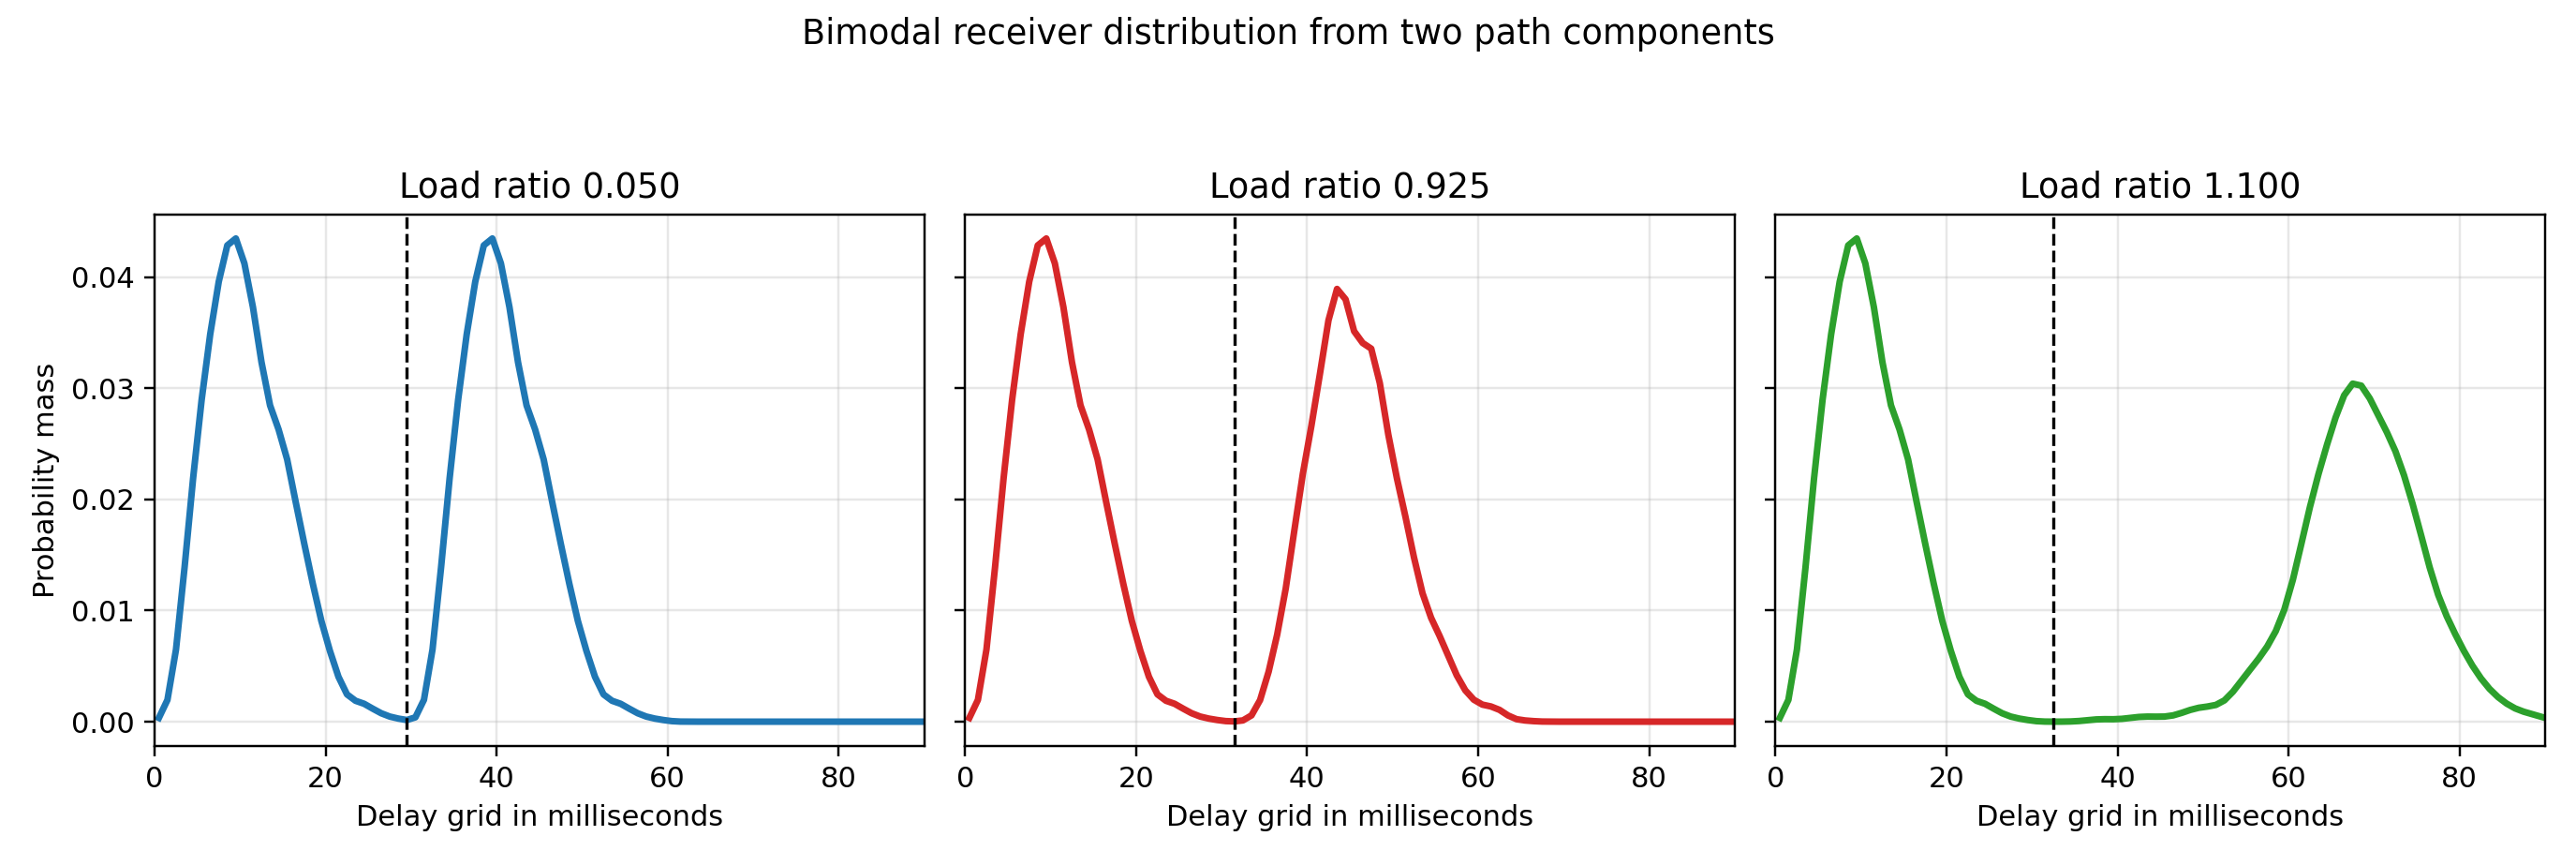
\includegraphics[width=\textwidth]{multipath_bimodal_example.png}
\caption{Example bimodal receiver distribution for a two-component path mixture. The dashed line is the valley split used to separate the lower-delay and upper-delay modes.}
\label{fig:multipath-bimodal-example}
\end{figure}

The modal split is stable under the constructed experiment. Across all traffic shares and all three delay families, the low-load mixture is detected as bimodal in all 1,200 cases. The median split is 29.5 milliseconds for the lognormal and Weibull mixtures, and 57.5 milliseconds for the normal mixtures. The difference is a consequence of the underlying single-link delay shape and the 30 millisecond path offset, rather than a change in the decision rule.

Figure \ref{fig:multipath-component-response} shows the component response for the Weibull case at \(\alpha=0.50\). The whole mixture has a visible TVD jump near the same region as the single-path boundary, but it is smaller because only half the probability mass belongs to the changing component. The lower mode remains close to zero TVD across the sweep. The upper mode shows the sharp response, and its rate-change boundary is the same 0.925 load-grid point selected in the single-link and multi-hop chapters.

\begin{figure}[htbp]
\centering
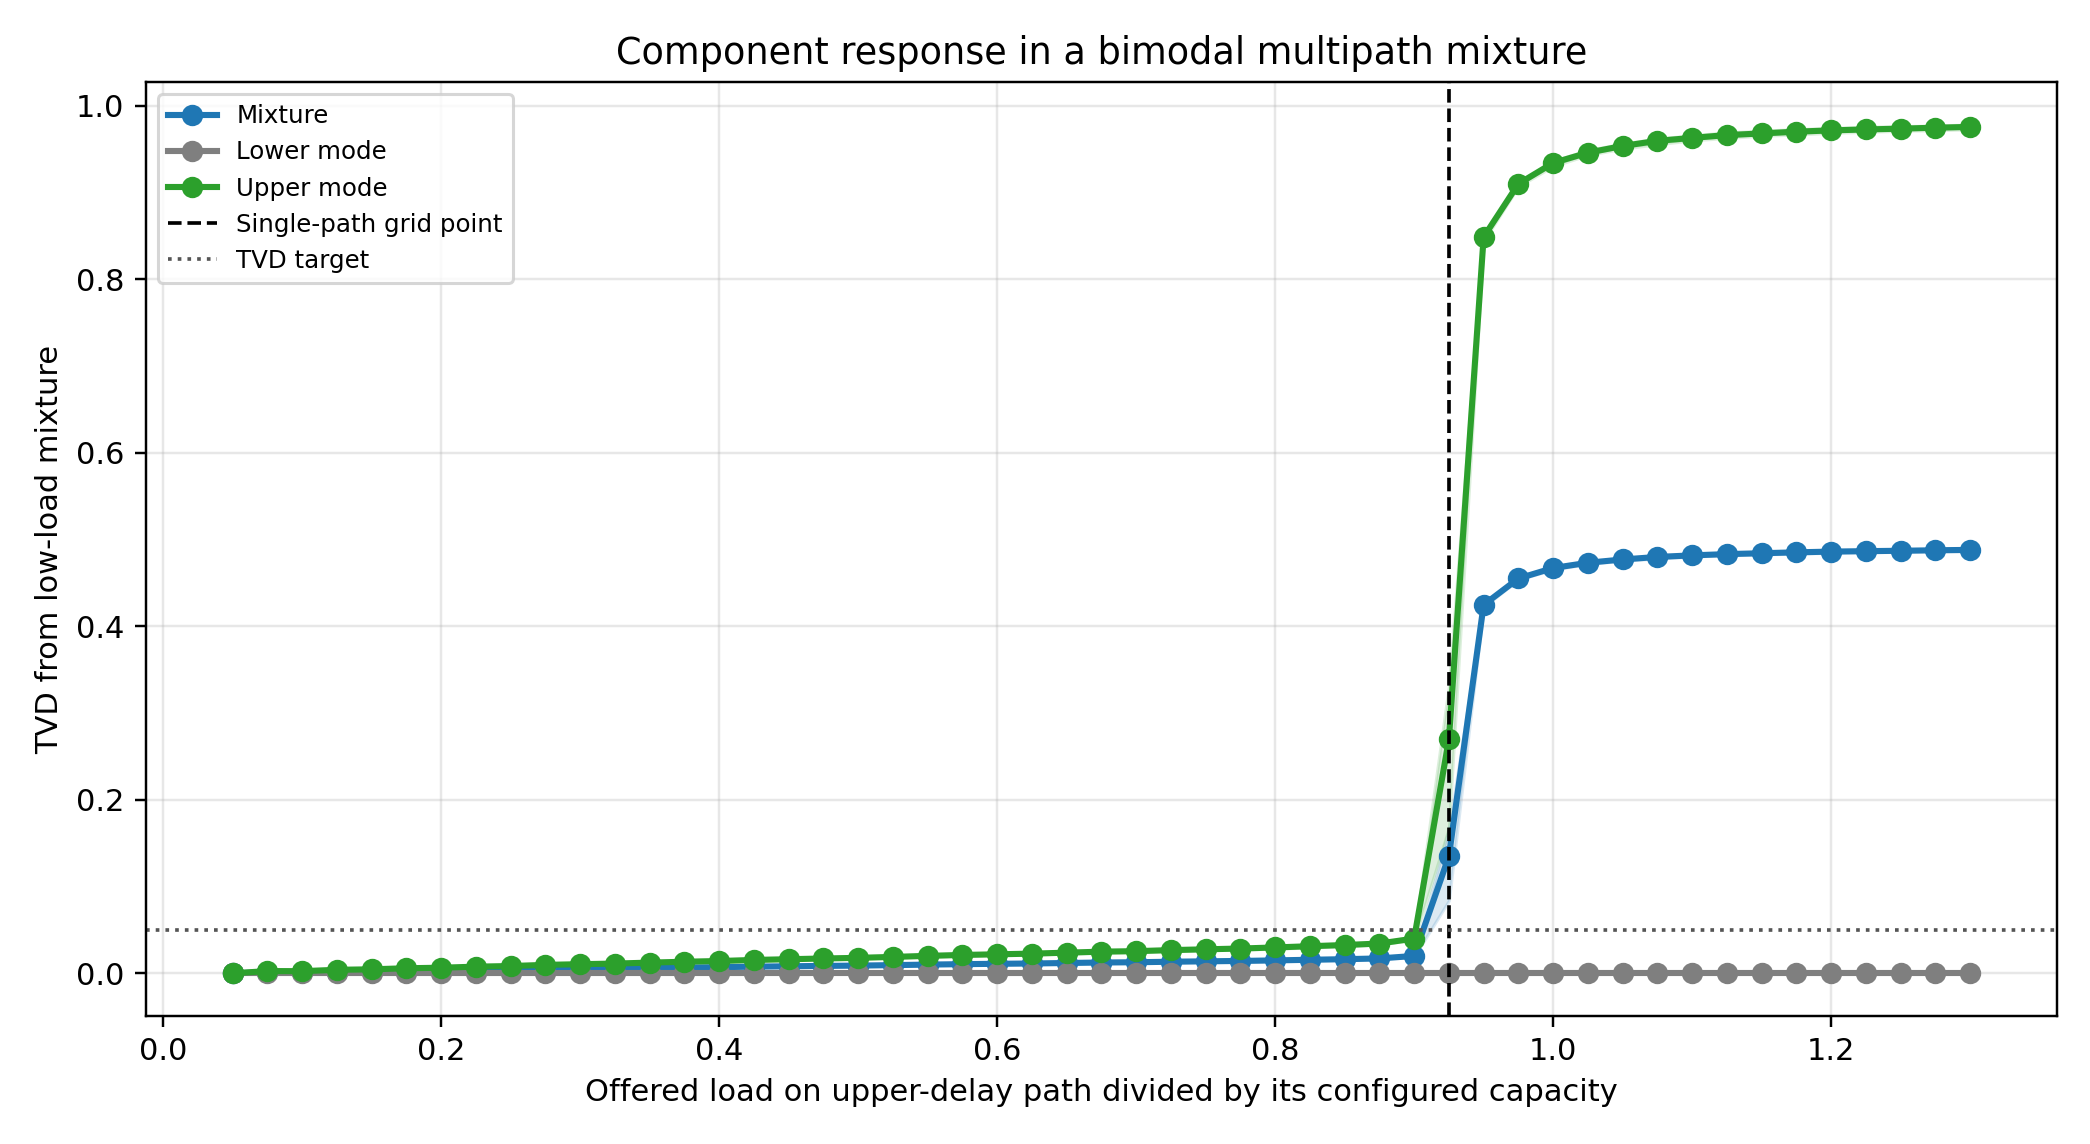
\includegraphics[width=\textwidth]{multipath_component_response_weibull_share50.png}
\caption{Median TVD response in the bimodal Weibull mixture with a 50 percent upper-path share. The upper component carries the capacity response while the lower component remains stable.}
\label{fig:multipath-component-response}
\end{figure}

Table \ref{tab:multipath-methods} summarises the detection results across traffic shares. The whole-mixture criteria are not reliable across the full range. At \(\alpha=0.10\), the mixture rate-change rule detects a boundary in only 69.7 percent of runs, and its median detected ratio among successful detections is 0.950. The stressed path is present, but its contribution to the whole distribution is too small to produce a consistent mixture-level acceleration. At \(\alpha=0.75\), the mixture first-change rule detects too early, with a median of 0.800 and 66.3 percent of runs below 0.900. The mixture is then dominated by the stressed path, so ordinary pre-boundary movement is mistaken for capacity.

\begin{table}[htbp]
\centering
\small
\begin{tabular}{p{0.18\textwidth}p{0.26\textwidth}rrp{0.19\textwidth}}
\toprule
Traffic share on upper path & Criterion & Detection rate & Median ratio & Interquartile range \\
\midrule
0.10 & Mixture first change & 1.000 & 0.950 & 0.925 to 0.950 \\
0.10 & Mixture TVD rate & 0.697 & 0.950 & 0.925 to 0.950 \\
0.10 & Upper-mode TVD rate & 1.000 & 0.925 & 0.925 to 0.925 \\
0.25 & Mixture first change & 1.000 & 0.925 & 0.925 to 0.925 \\
0.25 & Mixture TVD rate & 1.000 & 0.925 & 0.925 to 0.925 \\
0.25 & Upper-mode TVD rate & 1.000 & 0.925 & 0.925 to 0.925 \\
0.50 & Mixture first change & 1.000 & 0.925 & 0.925 to 0.925 \\
0.50 & Mixture TVD rate & 1.000 & 0.925 & 0.925 to 0.925 \\
0.50 & Upper-mode TVD rate & 1.000 & 0.925 & 0.925 to 0.925 \\
0.75 & Mixture first change & 1.000 & 0.800 & 0.750 to 0.925 \\
0.75 & Mixture TVD rate & 1.000 & 0.925 & 0.925 to 0.925 \\
0.75 & Upper-mode TVD rate & 1.000 & 0.925 & 0.925 to 0.925 \\
\bottomrule
\end{tabular}
\caption{Multi-path mixture detection results over normal, lognormal, and Weibull families with 100 seeds each. The lower-mode TVD rate did not fire in any run, so it is omitted from the table body.}
\label{tab:multipath-methods}
\end{table}

For every traffic share, the upper-mode response detects in all 300 runs associated with that share, with median 0.925 and interquartile range 0.925 to 0.925. These are not 1,200 independent confirmations of the capacity boundary, because the upper component is constructed from the single-link response. The result shows instead that the valley split recovers the embedded upper-path response cleanly across shares from 10 percent to 75 percent. The lower-mode response never fires, which is a sanity check on the construction: the unchanged component is not falsely assigned the capacity response.

Appendix Figure \ref{fig:multipath-methods} provides the corresponding summary plot. The table is kept as the main evidence because the detection rates and early detections are more important than the visual alignment of the bars.

The 30 millisecond offset is also tested directly because modal separation is the chapter's main free parameter. Figure \ref{fig:multipath-offset-sensitivity} and Table \ref{tab:multipath-offset-sensitivity} sweep the offset from 10 to 50 milliseconds. At 10 milliseconds, only 66.7 percent of cases pass the bimodal-split validity check. At 20 milliseconds this rises to 97.7 percent, and from 30 milliseconds onwards all tested cases have valid splits. Conditional on a valid split, the upper-mode median remains at 0.925 throughout the sweep. The offset plot is part of the evidence rather than a summary chart because it shows the failure boundary for the modal decomposition. The sweep supports the 30 millisecond setting as a separable proof-of-concept point, but it also shows where the approach begins to fail: insufficient delay separation prevents reliable component recovery.

\begin{figure}[htbp]
\centering
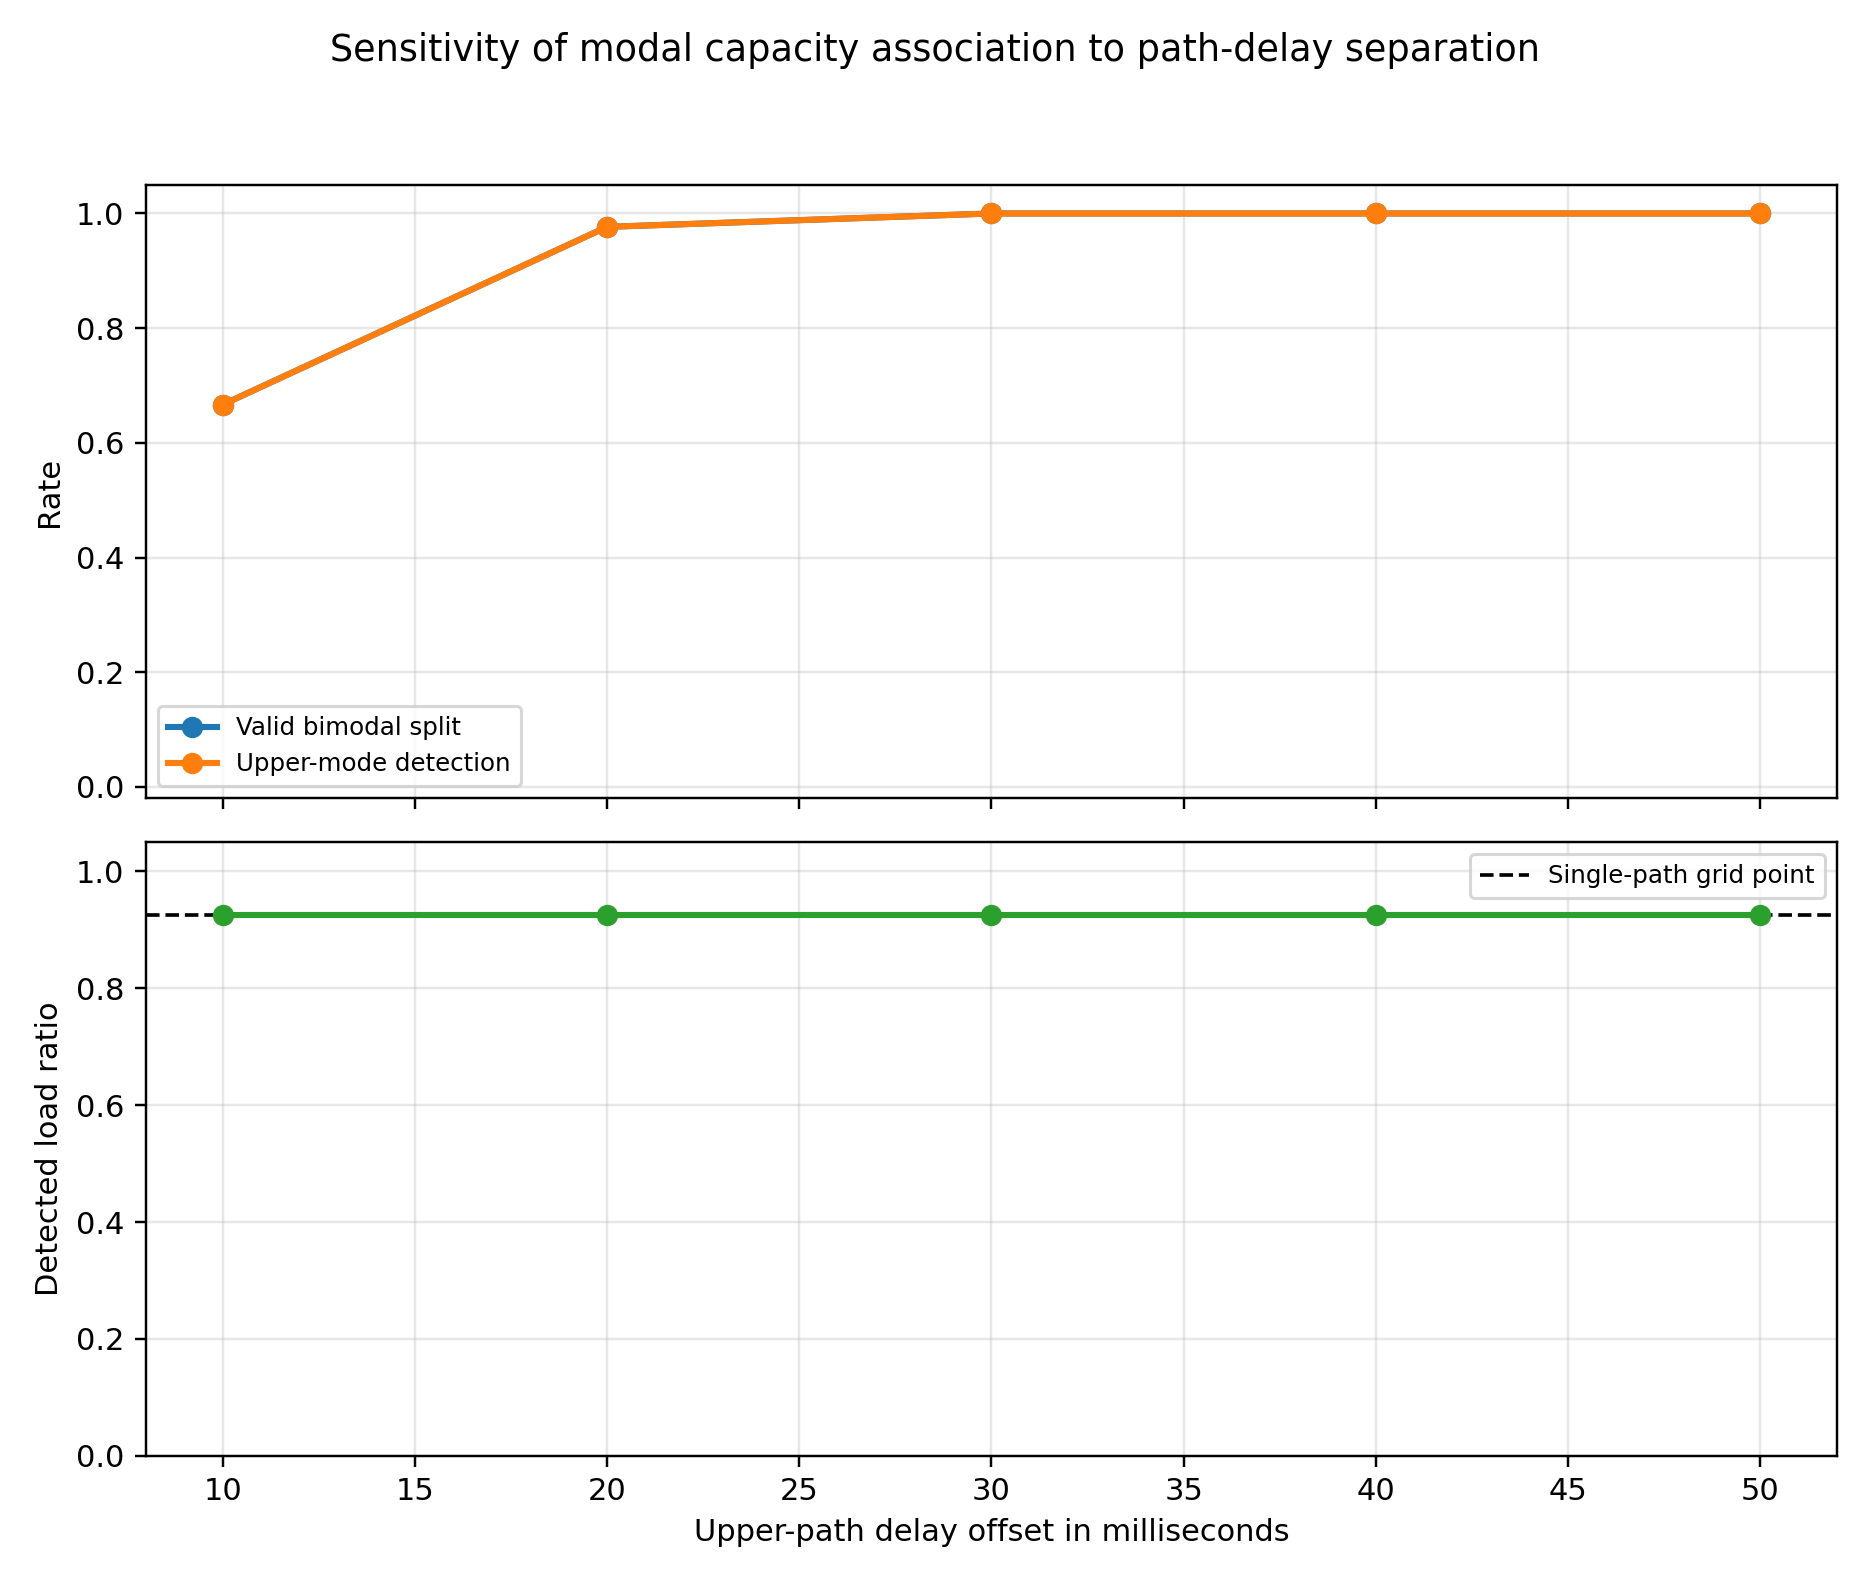
\includegraphics[width=\textwidth]{multipath_offset_sensitivity.png}
\caption{Sensitivity of modal capacity association to the delay separation between path components. Small offsets reduce the probability of a valid bimodal split, even though successful splits still recover the embedded upper-path response.}
\label{fig:multipath-offset-sensitivity}
\end{figure}

\begin{table}[htbp]
\centering
\small
\begin{tabular}{rrrrr}
\toprule
Offset in ms & Valid split rate & Upper detection rate & Median ratio & Late rate above 0.925 \\
\midrule
10 & 0.667 & 0.667 & 0.925 & 0.003 \\
20 & 0.977 & 0.977 & 0.925 & 0.016 \\
30 & 1.000 & 1.000 & 0.925 & 0.013 \\
40 & 1.000 & 1.000 & 0.925 & 0.013 \\
50 & 1.000 & 1.000 & 0.925 & 0.013 \\
\bottomrule
\end{tabular}
\caption{Offset sensitivity for the multi-path modal split over all tested shares, distributions, and seeds.}
\label{tab:multipath-offset-sensitivity}
\end{table}

\section{Interpretation}

The multi-path experiment shows that the response-rate criterion can be attached to a modal component when the receiver distribution is a separable mixture. It also identifies a separate failure mode from the previous chapters. In the single-link chapter, first-change detection is too sensitive to delay family. In the multi-hop chapter, first-change detection collapses as path length increases. In the multi-path chapter, whole-mixture TVD is diluted at low stressed-path share and too sensitive at high stressed-path share. Modal decomposition preserves the distributional signal without collapsing different path behaviours into one score.

The experiment does not yet prove a deployable multi-path monitor. It is constructed from saved stopped distributions rather than from a routed NS-3 equal-cost multi-path topology, and the 30 millisecond offset makes the two modes separable by design. The result demonstrates the statistical decision without making an operational claim about arbitrary multi-path networks. It tests the statistical decision of identifying which mode carries capacity pressure in an already-mixed receiver distribution. It does not test load balancing, path selection, per-flow hashing, packet reordering, or shared-queue interactions, which would require a routed NS-3 multi-path topology. If the path-delay modes overlap strongly, a valley split may be unstable and a formal unimodality test, a bootstrap mode-count test, or a mixture model would be needed before assigning capacity responses to components.

In this restricted setting, the modal split separates the receiver-side distribution into interpretable components, identifies which component is changing, and associates the capacity response with that component. The offset sweep makes the limitation explicit: the method is reliable when the route components are sufficiently separated, and unreliable when the modes overlap enough that the split cannot be recovered consistently.

\chapter{Scope and Limitations}
\label{sec:scope-limitations}

The evaluation is intentionally controlled, and the claims are bounded by that scope. All network experiments use Network Simulator 3 rather than a hardware testbed or production trace. This makes the hidden link rate, traffic load, and delay family available for post-hoc scoring. The results do not yet include clock noise, operating-system timestamp artefacts, real traffic mixes, routing churn, or device-specific queue behaviour.

The main single-link and multi-hop capacity experiments use stationary constant-bit-rate cross traffic and finite first-in, first-out queues. A bursty Pareto on-off stress test is added for the single link, but it remains synthetic User Datagram Protocol traffic rather than Transmission Control Protocol feedback, application traffic, or adversarial background traffic. The comparison with packet loss is also limited by the 0.025 load grid: in the constant-rate experiments, the distributional boundary appears one grid step before endpoint cross-traffic loss, which is the smallest non-zero timing gap the experiment can resolve.

The multi-hop experiment is primarily a depth-invariance test under uniform load. Every link in the main run has the same 10 Mbit/s configured rate, and the cross traffic enters at the first node and exits at the last node. The heterogeneous five-hop stress test adds one slow link at the first, middle, or final position, but it still uses one end-to-end traffic source and one controlled slow link. A real topology could have intermediate cross-traffic entry and exit points, several independent queues changing at different rates, or several bottlenecks that appear and disappear over time.

The distributional assumptions are also bounded. The main network experiments use three continuous delay families: normal, lognormal, and Weibull. These are useful representatives of symmetric, skewed, and asymmetric positive delays, but they do not establish invariance across all delay processes. The multi-path chapter adds a constructed two-component mixture, not a routed equal-cost multi-path simulation with flow hashing, reordering, or shared bottlenecks. Its result is therefore evidence that modal decomposition can recover an embedded capacity response when the modes are separable, not proof that arbitrary multi-path routing can be inferred from passive delay alone.

Finally, several implementation choices remain fixed throughout the evaluation. Continuous distributions are compared on a 1 millisecond grid from 0 milliseconds to 150 milliseconds, KDE uses Scott's rule for bandwidth selection, and the capacity boundary is reported on a 0.025 load grid. The parameter sensitivity plots show that the response-rate multiplier is not solely responsible for the 0.925 boundary, the bursty experiment shows that the detected average-load boundary depends on the traffic process, the heterogeneous stress test checks one slow-link position at a time, and the multi-path offset sweep characterises one modal-separation parameter. Broader robustness still requires bin-resolution sensitivity, richer traffic traces, multiple simultaneous bottlenecks, and routed multi-path experiments.

The response-rate criterion also has identifiable failure modes. It should fail when the low-load TVD baseline is already unstable, when traffic changes non-monotonically during the sweep, when routing changes while the monitor is collecting a load point, or when several bottlenecks produce multiple smaller bends rather than one sharp acceleration. These cases are not defects in the implementation; they define the boundary between a controlled capacity-pressure experiment and a deployable monitoring policy.

\chapter{Future Work}

The experiments in this report stop at controlled capacity-boundary problems. That makes the contribution easier to evaluate and positions the method as a foundation rather than a complete monitoring system. The reusable part is the pipeline: reconstruct a receiver-visible delay distribution, stop when that reconstruction is stable, compare it with an empirical operating state, and interpret the rate of distributional change. The multi-path chapter adds a fourth step when needed, which is to decompose the receiver distribution into modal components before associating a boundary with one path behaviour. The same pipeline can be applied to several related monitoring problems where the key signal is how the full delay distribution changes over time, across paths, or under intervention.

\section{Path Profiling and Rerouting}

The most direct extension is path profiling. In a network with several possible routes between a source and destination, each path can be associated with a characteristic delay distribution. If a failure or routing update moves a flow onto another path, the receiver may observe a shift in the distribution even when no explicit failure alarm is raised. This connects naturally to data-centre and wide-area traffic engineering, where systems such as Hedera, B4, SWAN, and CONGA already exploit path diversity and load balancing to improve utilisation or respond to congestion \cite{alFaresHedera,jainB4,hongSwan,alizadehConga}.

The method in this report could support a passive version of that reasoning. Instead of requiring the monitor to know the selected route, it could compare the current stopped distribution with a library of previously learnt path profiles. A post-failure distribution that matches one profile more closely than another would give evidence about where the flow has moved. Routing telemetry would still be more direct, but the distributional comparison could provide an independent receiver-side check that rebalancing has actually changed the observed path behaviour. The multi-hop and multi-path results are the relevant starting point because they show that a path-level distribution can remain interpretable when several links contribute to delay, and that separable route components can be analysed through their modes. A full routed equal-cost multi-path or unequal-cost multi-path implementation remains future work because the experiment here constructs mixtures from stopped path components rather than simulating router-level path splitting.

\section{Failure Recovery and Healing}

Another extension is to use distributional profiles to distinguish between different recovery mechanisms after a failure. A path may improve because Transmission Control Protocol flows slow down, because traffic is rebalanced across paths, or because a failed component has been repaired. These cases can have different distributional signatures. A pure throughput counter or scalar alarm may report improvement in all three cases, while the delay distribution could reveal whether the path has returned to its earlier shape or has settled into a different operating state.

Such a monitor would complement systems such as Pingmesh, Everflow, NetSight, and Fathom, which make failures and performance regressions more observable through active measurements, packet tracing, or application-level latency decomposition \cite{guoPingmesh,zhuEverflow,handigolNetSight,qureshiFathom}. The future-work question is whether the stopped delay distribution can act as a compact behavioural fingerprint for healing. The method would need a stronger identity step than the one used here, because the task would not only be to detect change. It would also be to decide whether the post-event distribution has returned to the pre-event state or converged to a new stable state.

\section{Short Events and Transient Change}

Short events are a harder use case because adaptive stopping waits for evidence that a distribution is stable. Micro-bursts, sub-second congestion, and transient queue build-up may disappear before enough samples have been collected for the conservative stopping rule used in this report. Existing work such as Trumpet, \(\mu\)Mon, Packet Doppler, and DRILL shows that short-timescale behaviour matters in data-centre networks and that microsecond or millisecond events can affect performance before slower counters react \cite{moshrefTrumpet,zhengMuMon,qiuPacketDoppler,ghorbaniDrill}.

A distributional extension would therefore need to change the stopping model. Instead of asking for one stable distribution over a long interval, the monitor could maintain rolling or hierarchical distributions at several time scales. A short event would then be detected as a temporary movement of mass into a higher-delay region, a temporary tail expansion, or a short-lived second mode. The statistical challenge is to avoid treating ordinary sampling noise as an event. The failed \(B=100,\theta=\delta\) stopping cases in the adaptive-stopping chapter are relevant here because they show exactly how under-sampled distributions can look deceptively stable. Any short-event version of this work would need explicit false-alarm control.

\section{Capacity Aware Backup Path Testing}

The capacity-boundary method can also be applied to backup-path testing. Operators often need to know whether a standby path can absorb traffic during a failure or grey failure without immediately degrading delay. Active available-bandwidth tools such as Pathload, PathChirp, and Spruce estimate path capacity or available bandwidth using probe traffic \cite{jainDovrolisPathload,ribeiroPathchirp,straussSpruce}. The approach in this report suggests a complementary experiment: increase offered load on a candidate backup path, reconstruct stopped delay distributions at each load, and detect the point where the response accelerates.

That extension would turn the current single-path experiment into a path-comparison tool. Two paths might have the same nominal link rate but different delay response curves, tail behaviour, or sensitivity to added traffic. A distributional capacity boundary could therefore help choose whether a backup path has enough capacity and which backup path preserves the most stable delay behaviour under load. The method would need careful guardrails because the test traffic itself can consume headroom. The additive-increase result in this report is relevant because it approaches the boundary more gently than a binary search and keeps the response curve visible.

\section{Induced Change and Configuration Testing}

The use case also extends to planned interventions. Introducing a new load balancer, changing a routing policy, or modifying traffic classes may change the shape of the delay distribution even when no immediate failure occurs. Systems such as B4 and SWAN show that traffic-engineering systems can intentionally push networks towards high utilisation, while relying on control logic to avoid harmful transients \cite{jainB4,hongSwan}. A distributional monitor could provide a before-and-after test for whether such an intervention changes the operating regime seen by end hosts.

The current pipeline supplies the first part of this design. It shows how to compare stopped distributions and why a first-change rule can be too sensitive. Future work should separate benign induced change from harmful induced change. A load-balancer update may intentionally move traffic onto a different path, so a distributional difference is not automatically bad. The richer question is whether the new distribution has a heavier tail, a sharper response-rate boundary, or less headroom before delay behaviour deteriorates. Distributional profiling would then help judge the quality of a change, rather than only detecting that a change occurred.

\section{Telemetry Assisted Validation}

The final extension is to combine passive distributional monitoring with richer telemetry when it is available. In-band network telemetry, PINT, Marple, ConQuest, and UnivMon demonstrate that programmable or sketch-based measurement can expose queue state, hop latency, flow contributions, and network-wide summaries more directly than receiver-side delay alone \cite{p4IntSpec,benBasatPint,narayanaMarple,chenConQuest,liuUnivMon}. The method in this report is weaker by design because it does not assume that instrumentation. That weakness can become useful in a validation setting.

Telemetry could provide ground truth for why a distributional boundary appears. If the delay distribution accelerates at a particular load, switch-local queue or hop-latency measurements could show whether the cause was one congested link, several lightly stressed links, or a routing change. Conversely, if telemetry reports queue pressure but the receiver-side distribution does not change, that would reveal a limit of the passive method. This pairing would make the work more deployable: passive distributional monitoring could run continuously at low overhead, while richer telemetry could be triggered when the distributional signal indicates that a path has entered a new regime.

\chapter{Conclusion}

This report has evaluated whether passive delay distributions can support a capacity-boundary decision. The motivation was that network operators often have to reason about remaining path capacity from limited observations, while scalar metrics such as mean delay, percentile latency, or link utilisation can hide important changes in distributional shape. The central question was therefore whether a monitor that only sees receiver-side packet delays can reconstruct the delay distribution, decide when that reconstruction is stable, and use distributional change to infer when a path leaves its previous operating regime.

The statistical evaluation establishes the foundation. Finite-domain distribution learning gives a conservative reference bound for reconstructing arbitrary distributions in total variation distance. The empirical results show that the tested delay distributions are substantially easier than the worst case. In the discrete setting, binomial and Zipfian distributions reach the 0.05 TVD target with about ten times fewer samples than the theoretical reference, while the irregular piecewise distribution is harder but still reaches the target well before the bound. In the continuous setting, kernel density estimation is more sample-efficient than a binned empirical probability mass function because it exploits smoothness across neighbouring delay values.

The adaptive stopping evaluation then converts offline reconstruction into an online decision. The monitor cannot observe ground truth at deployment time, so it needs a rule based only on consecutive estimates. The experiments show that loose stopping thresholds can stop too early, because two under-sampled estimates can be close to one another without either being accurate. The conservative continuous configuration \(B=200,\theta=\delta/6\) avoids that failure across the tested normal, lognormal, and Weibull distributions while keeping the median stopping cost far below the theoretical sample count.

The capacity experiments reject the initial intuition that first distributional change should mark the capacity boundary. In the single-link experiment, first-change detection fires at a median of 0.625 of configured capacity because some delay families move gradually under load. The stronger criterion is the rate at which TVD changes. It detects at the 0.925 load-grid point across all 300 constant-rate single-link runs, while endpoint cross-traffic loss appears later at 0.950, one load-grid step afterwards. Under Pareto on-off bursty traffic, the detected average-load boundary moves to 0.475 because the on-period sending rate is twice the swept average, and endpoint cross-traffic loss appears at a median of 0.575. The multi-hop experiment confirms that the constant-rate result is not only a clean one-link artefact under the tested path-wide load model. Across paths of two to ten hops and 2,700 runs, first-change detection becomes less meaningful as path length grows, while TVD rate change remains fixed at the same grid point. A heterogeneous five-hop stress test with one 10 Mbit/s slow link and four 20 Mbit/s links also recovers the 0.925 grid point when the slow link is first, middle, or final.

The constructed multi-path experiment adds a final qualification. When the receiver distribution is a separable mixture of route behaviours, whole-mixture TVD can either dilute the stressed component or react too early to ordinary movement in the dominant component. A modal split of the receiver distribution gives a cleaner association: the lower-delay mode remains stable, while the upper-delay mode recovers the embedded 0.925 load-grid response across all tested traffic shares. The offset sweep shows the boundary of this result: valid modal splits occur in only 66.7 percent of cases at a 10 millisecond path offset, but in all cases from 30 milliseconds onwards.

The project is best understood as a staged research argument. Theory first establishes what it means to learn a distribution. Direct sampling then shows that the tested delay shapes are learnable well below the worst-case bound. Adaptive stopping shows how to trust a reconstruction without ground truth. The first network use case then exposes a flaw in the naive identity interpretation and motivates the response-rate criterion. The multi-hop experiment tests that refined criterion under a harder path-level setting, and the multi-path experiment shows how the same idea must be attached to modal components when several route behaviours appear together.

This mirrors the system design introduced in Chapter 2. The pipeline stays fixed, but each evaluation stage tests one block more severely. The contribution is a bounded demonstration that a passive distributional monitor can be built from reconstruction, stopping, and comparison, and that the operational decision rule can be revised when an early hypothesis fails. The method does not measure exact physical link capacity, identify the responsible flow, or replace switch-local telemetry. The reported 0.925 boundary is an empirical result for the tested load grid, constant-rate traffic, finite queues, Scott's-rule kernel density estimates, separable modal mixtures, and the three continuous delay families evaluated here. The bursty stress test shows that the boundary should be interpreted through the offered traffic process, because average load and burst load can diverge.

The strongest conclusion is therefore foundational rather than final. The work establishes the components needed for a distribution-first passive monitor: finite-domain reconstruction, empirical stopping without ground truth, identity comparison against an observed operating state, response-rate detection after first-change failed, and modal association when receiver samples contain separable route behaviours. The future-work chapter follows directly from that foundation. Path profiling, rerouting checks, transient-event detection, configuration validation, and telemetry-assisted diagnosis all ask whether the same pipeline can be made practical beyond the controlled simulations evaluated here.

\appendix

\chapter{Supporting evaluation plots}

The appendix contains diagnostic plots used to check robustness of the main claims. Figures are grouped by the evaluation stage they support rather than by generation order.

\section{Statistical diagnostics}
\label{app:statistical-diagnostics}

\begin{figure}[htbp]
\centering
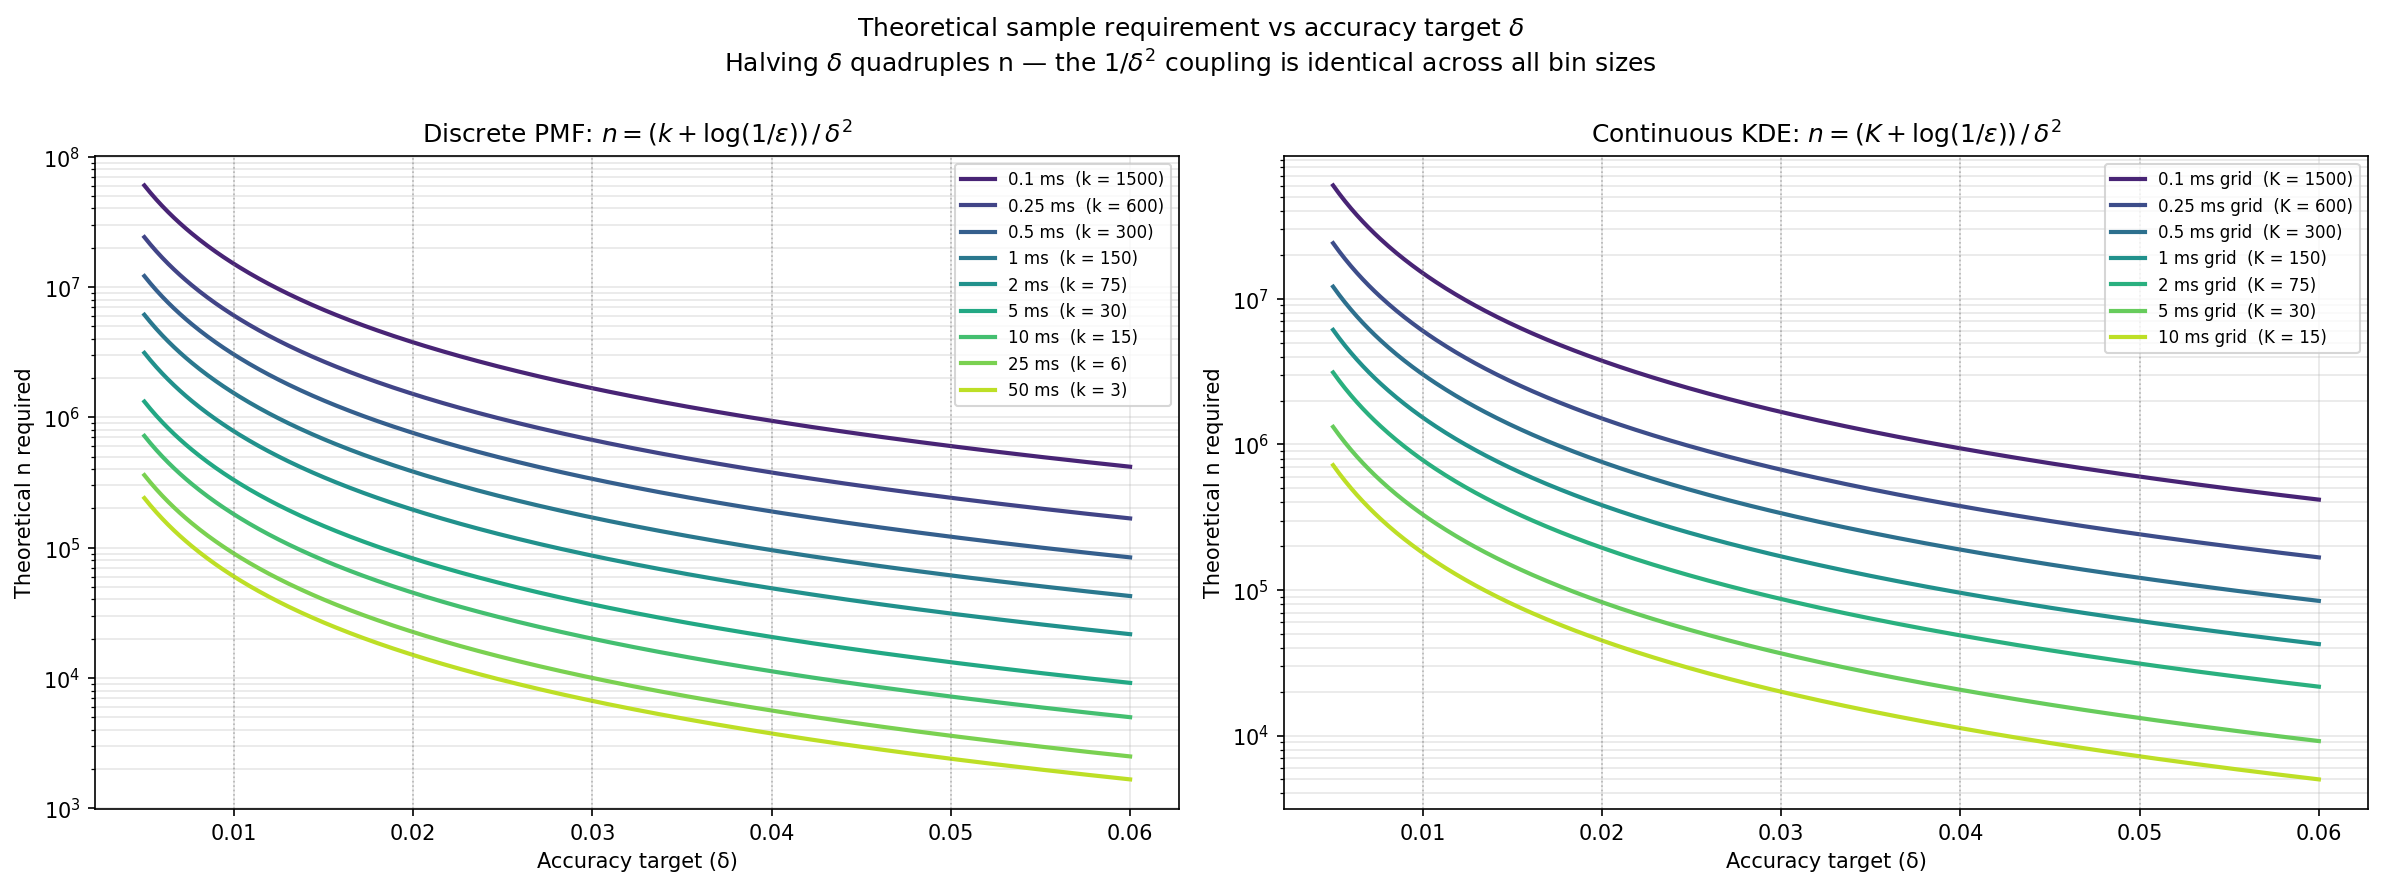
\includegraphics[width=\textwidth]{n_theory_vs_delta.png}
\caption{Theoretical sample requirement as the accuracy target changes. This plot makes the \(1/\delta^2\) coupling explicit for both PMF and KDE resolutions.}
\label{fig:app-n-theory-delta}
\end{figure}

\begin{figure}[htbp]
\centering
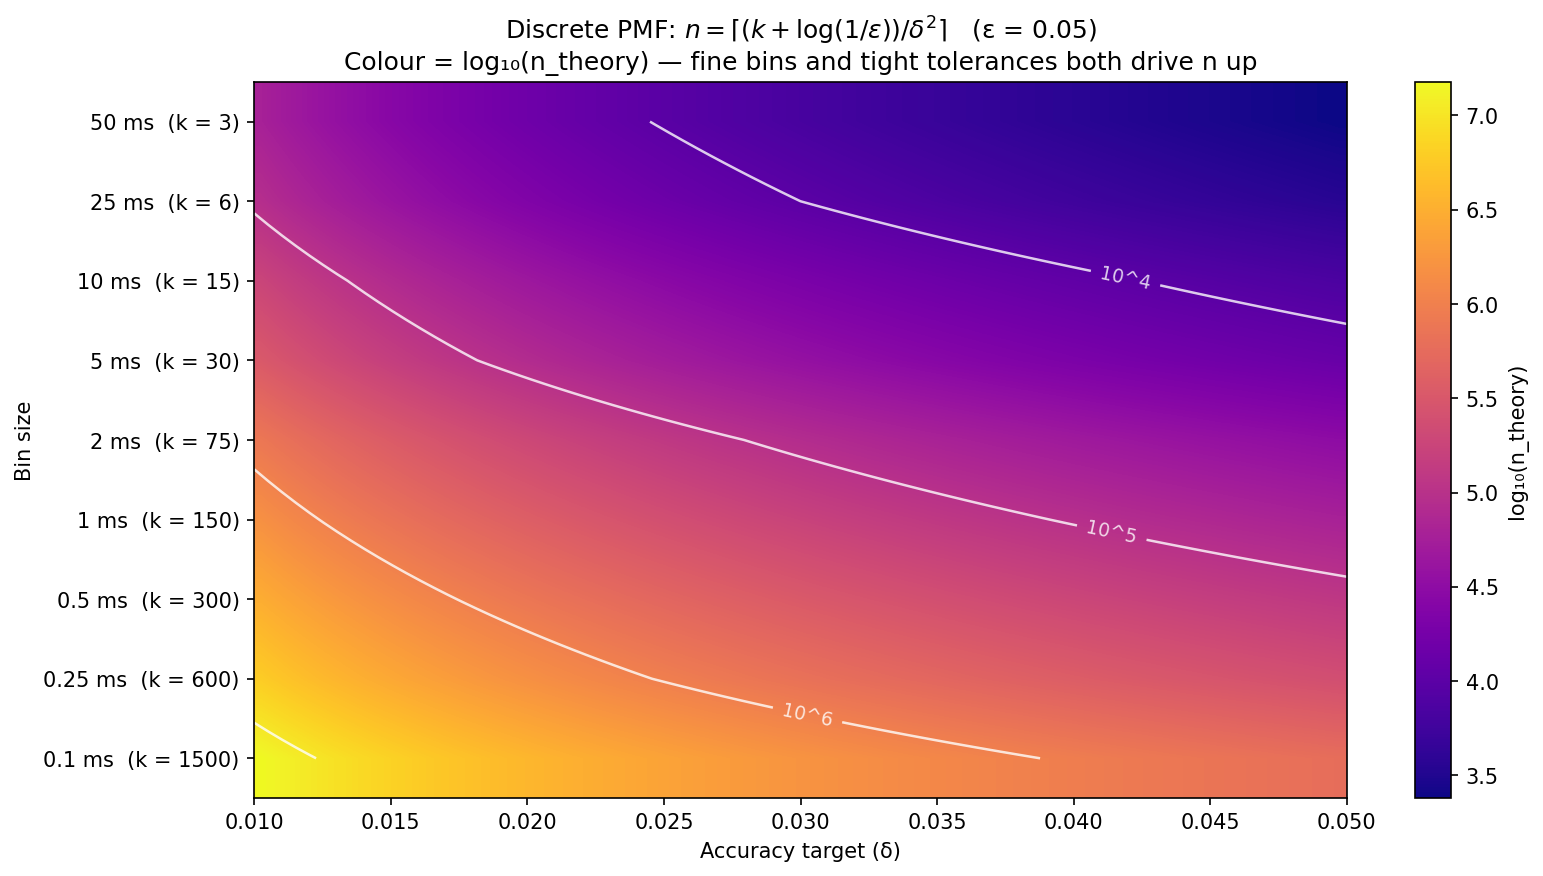
\includegraphics[width=\textwidth]{n_theory_heatmap.png}
\caption{Theoretical PMF sample requirement over bin size and TVD target. Very fine bins and tight error tolerances both drive the bound upwards.}
\label{fig:app-n-theory-heatmap}
\end{figure}

\begin{figure}[htbp]
\centering

\includegraphics[width=\textwidth]{tvd_vs_n_normal.png}
\caption{Median TVD against sample count for the normal distribution. This supporting view separates the normal curve from the combined continuous plot in the main text.}
\label{fig:app-tvd-vs-n-normal}
\end{figure}

\begin{figure}[htbp]
\centering

\includegraphics[width=\textwidth]{tvd_vs_n_lognormal.png}
\caption{Median TVD against sample count for the lognormal distribution. The right-skewed case remains easier than Weibull at the target accuracy.}
\label{fig:app-tvd-vs-n-lognormal}
\end{figure}

\begin{figure}[htbp]
\centering

\includegraphics[width=\textwidth]{tvd_vs_n_weibull.png}
\caption{Median TVD against sample count for the Weibull distribution. The interquartile band narrows as \(n\) increases.}
\label{fig:app-tvd-vs-n-weibull}
\end{figure}

\begin{figure}[htbp]
\centering
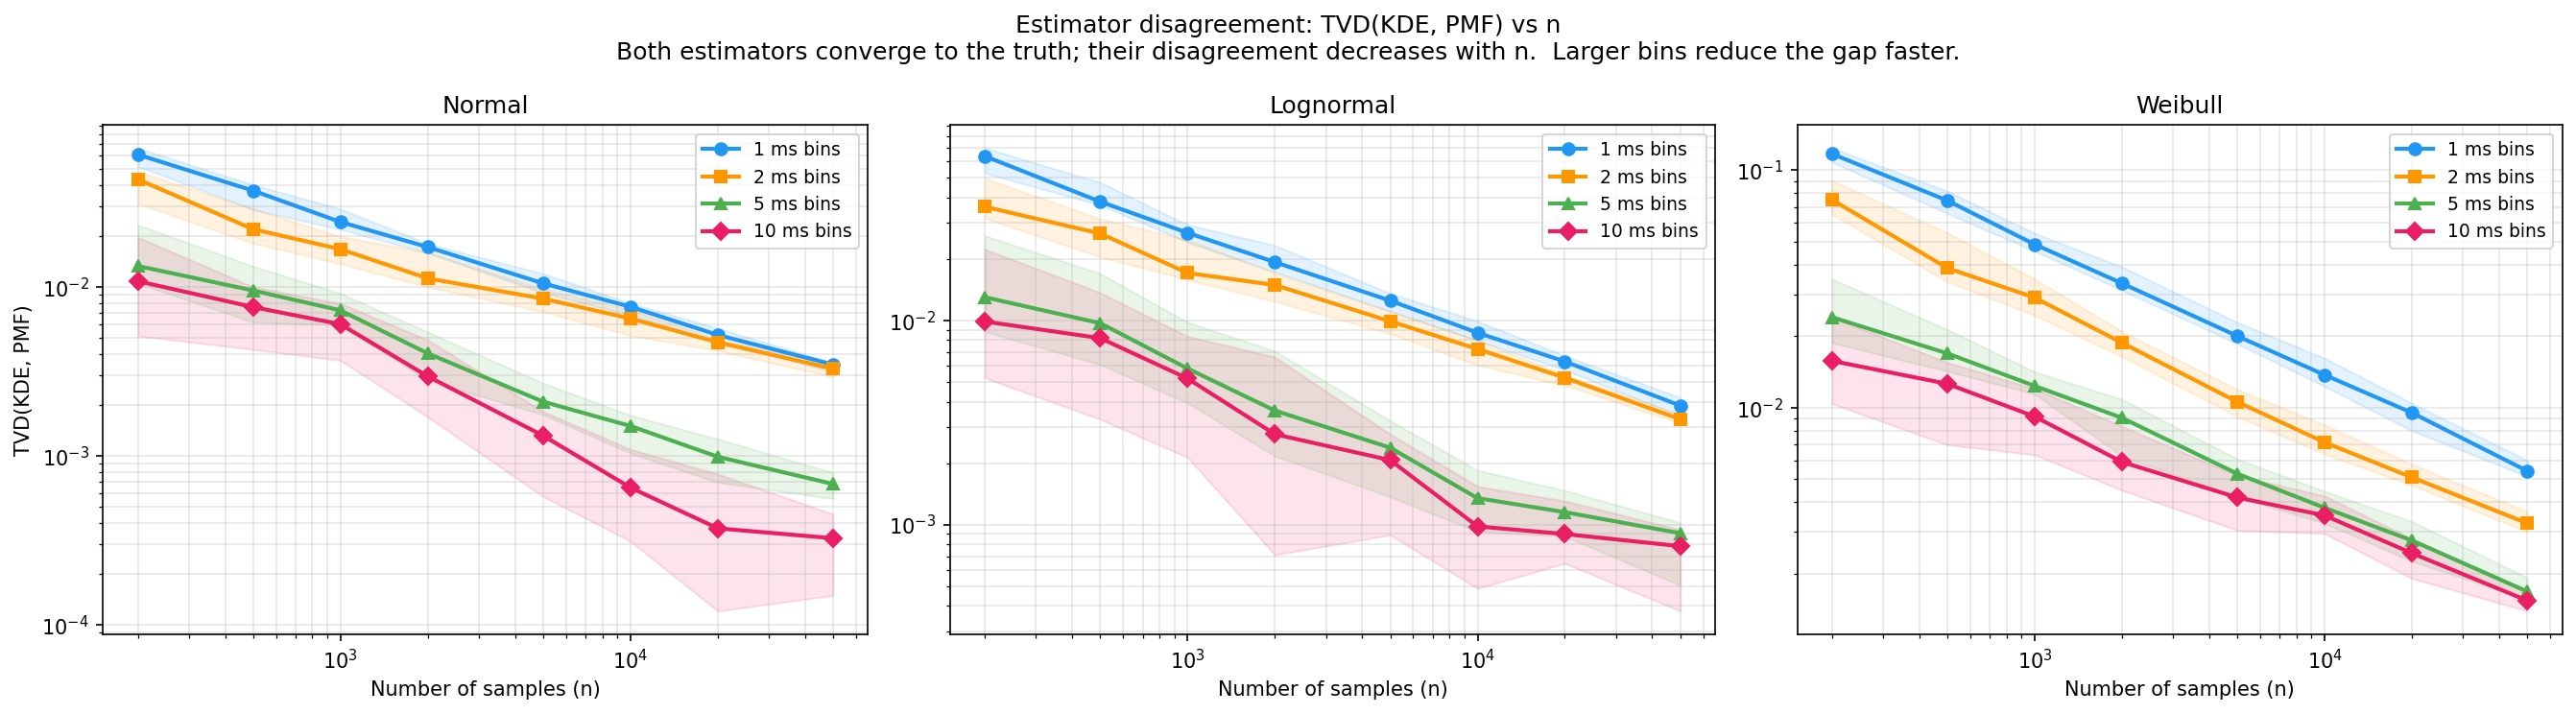
\includegraphics[width=\textwidth]{estimator_gap_all_dists.png}
\caption{TVD between the KDE and PMF estimates as the number of samples grows. The disagreement shrinks with \(n\).}
\label{fig:app-estimator-gap}
\end{figure}

\begin{figure}[htbp]
\centering
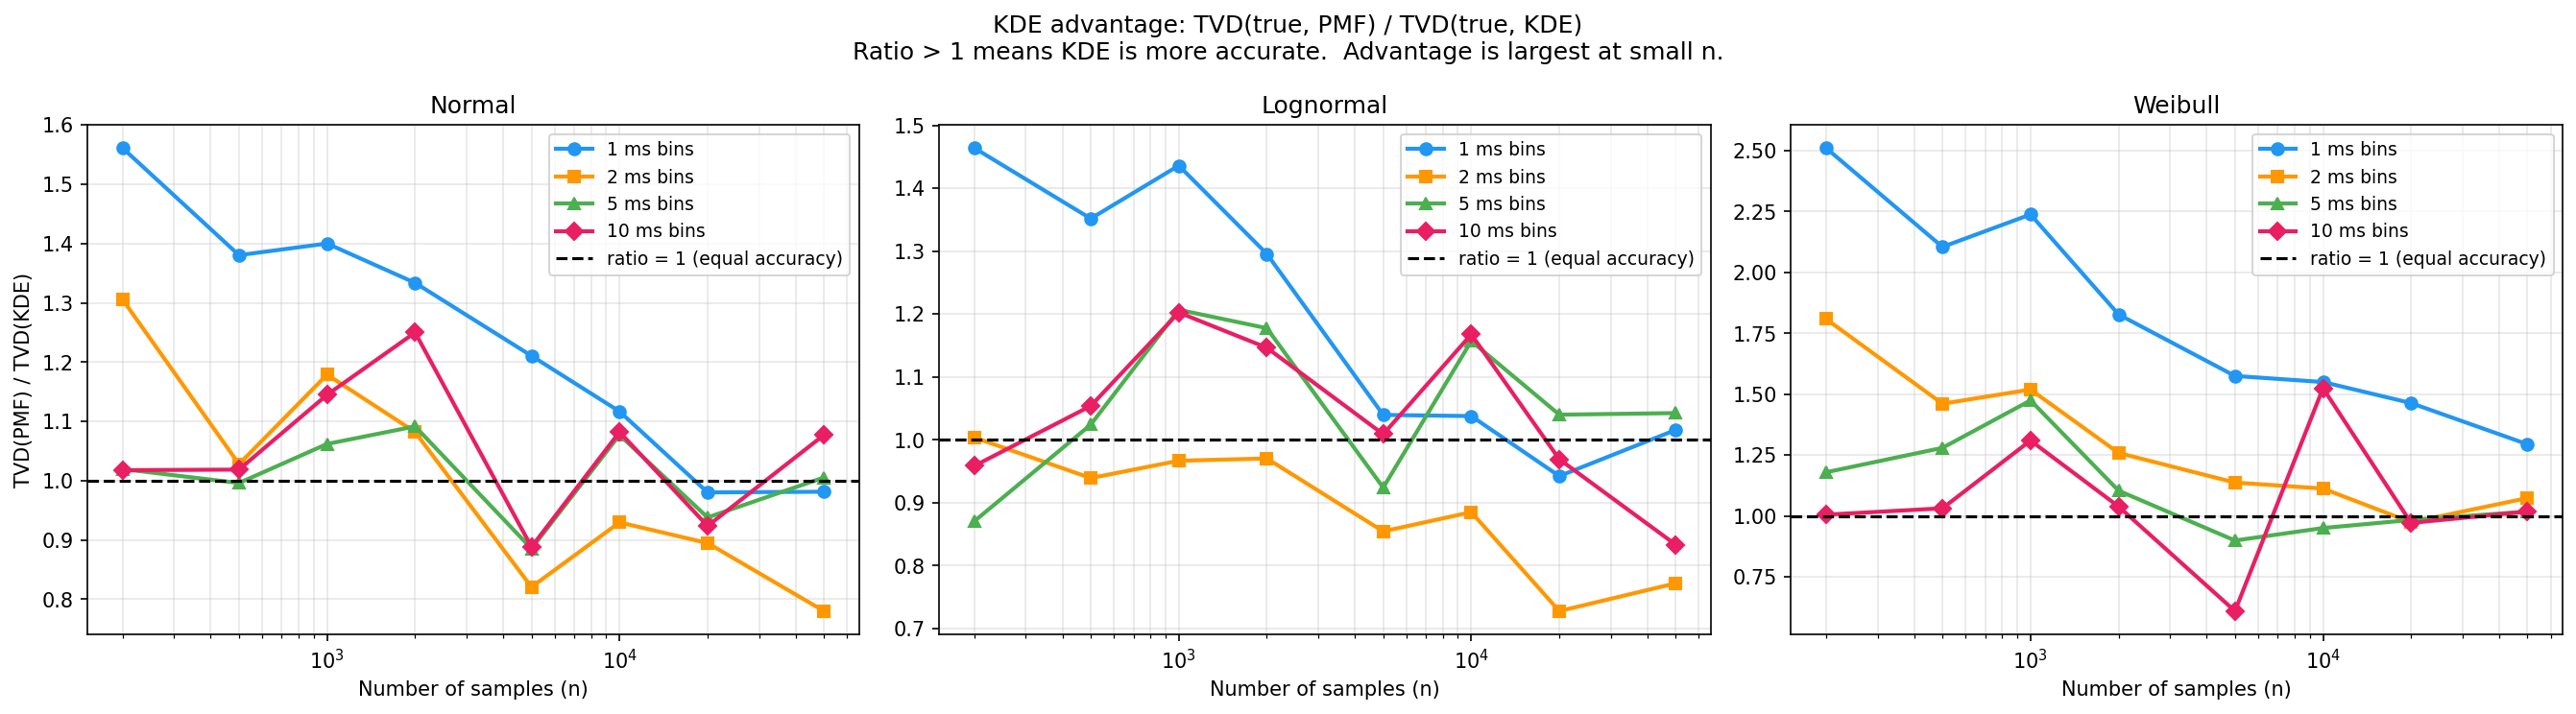
\includegraphics[width=\textwidth]{kde_advantage_ratio.png}
\caption{KDE advantage ratio, defined as TVD of PMF against truth divided by TVD of KDE against truth.}
\label{fig:app-kde-advantage}
\end{figure}

\begin{figure}[htbp]
\centering
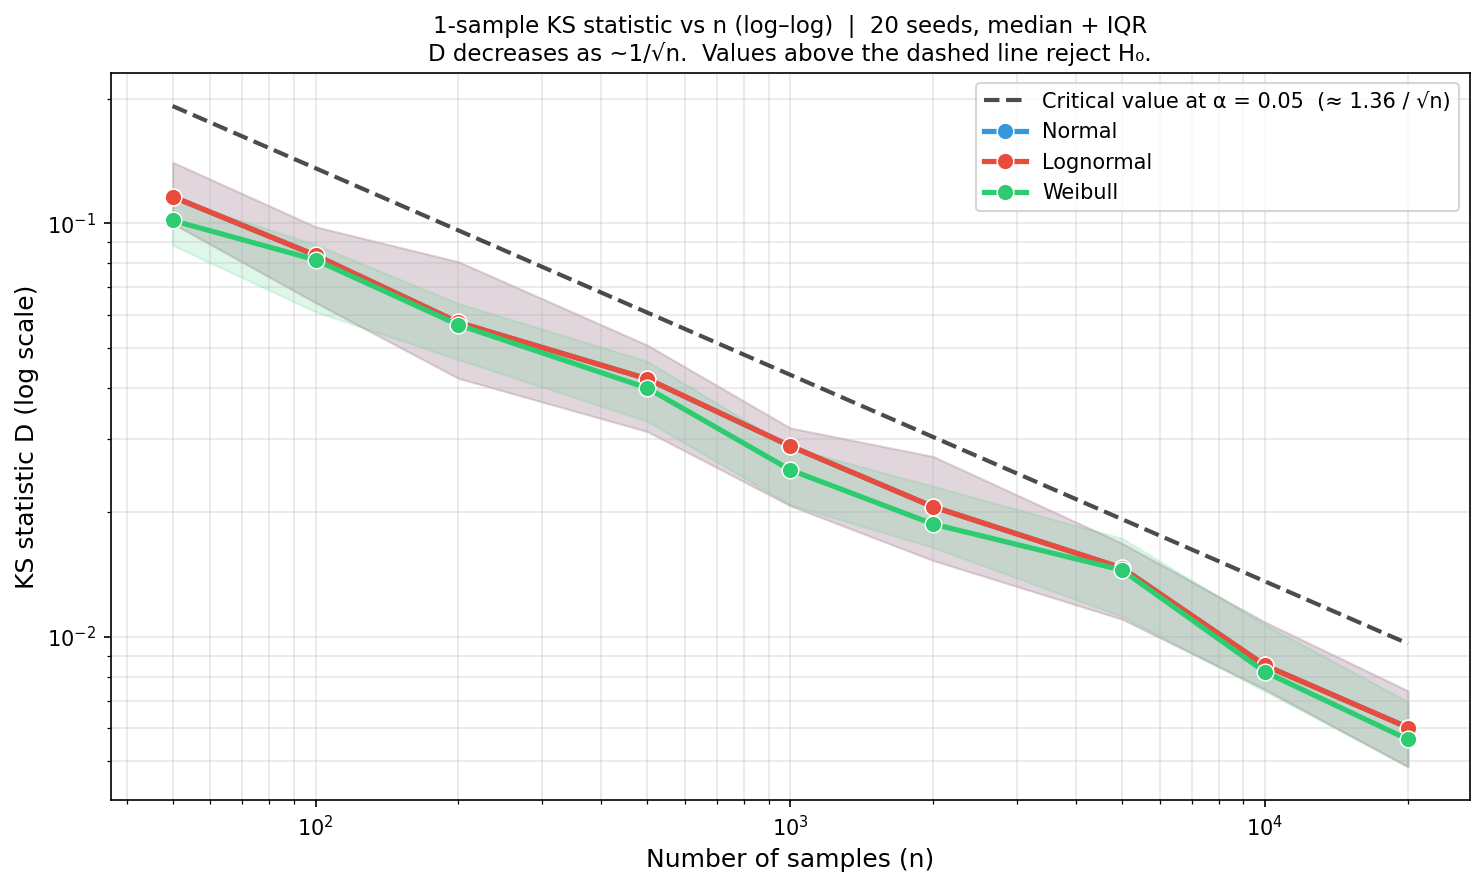
\includegraphics[width=\textwidth]{ks_statistic_vs_n.png}
\caption{One-sample Kolmogorov-Smirnov statistic as \(n\) increases.}
\label{fig:app-ks-statistic}
\end{figure}

\begin{figure}[htbp]
\centering
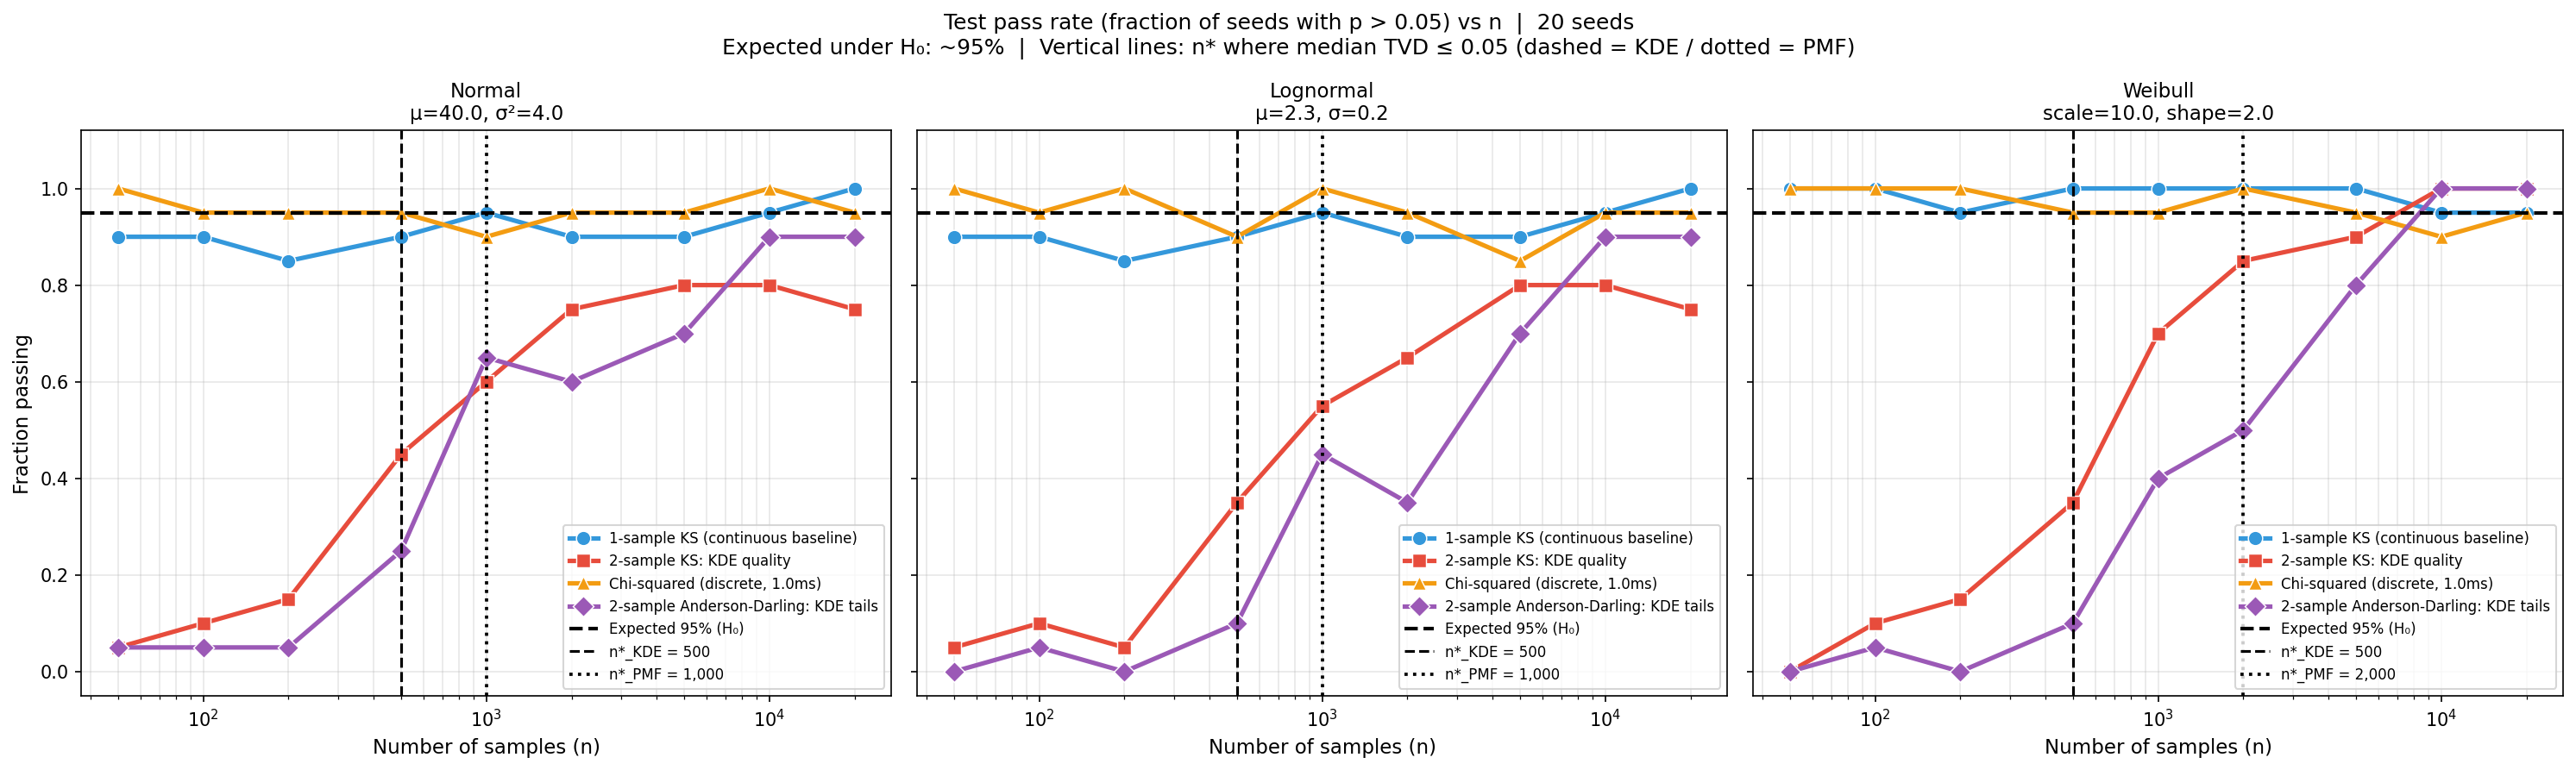
\includegraphics[width=\textwidth]{ks_pass_rate_vs_n.png}
\caption{Fraction of seeds passing each statistical test as \(n\) increases.}
\label{fig:app-ks-pass-rate}
\end{figure}

\clearpage

\section{Adaptive stopping diagnostics}
\label{app:adaptive-diagnostics}

\begin{figure}[htbp]
\centering
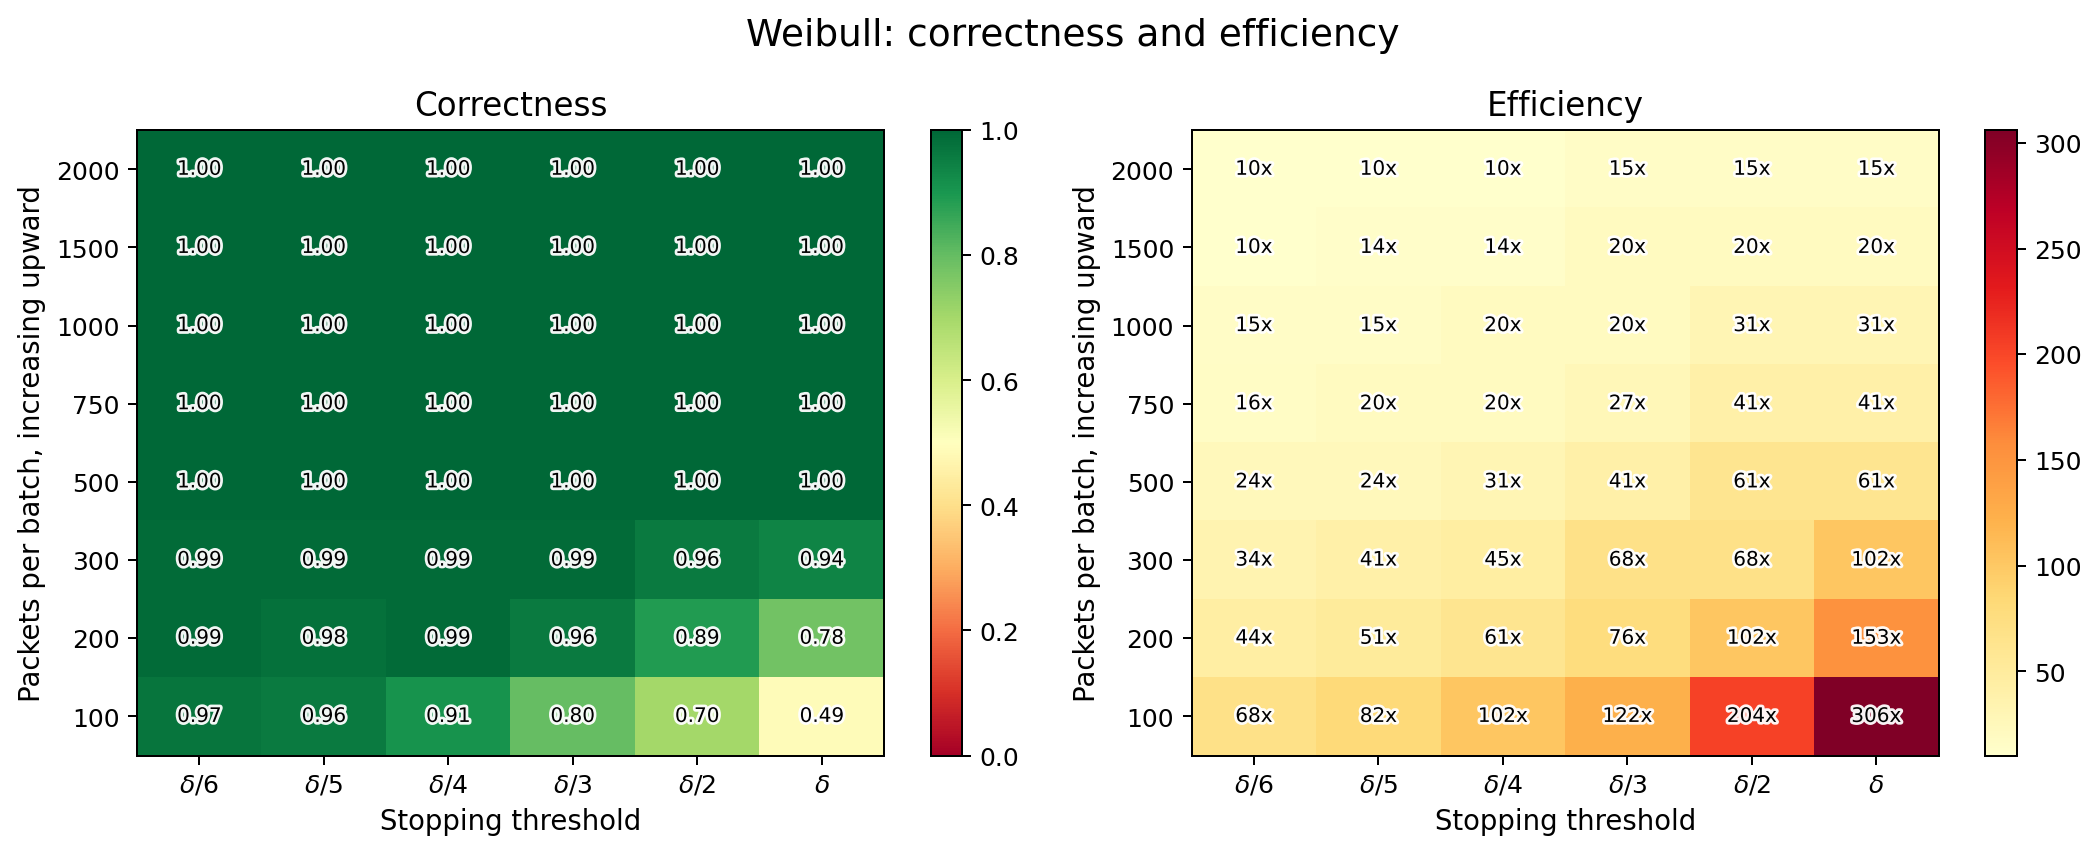
\includegraphics[width=\textwidth]{heatmap_cont_weibull.png}
\caption{Correctness and efficiency for the Weibull distribution. Efficiency is the ratio between the theoretical bound and the median stopping sample size.}
\label{fig:adaptive-weibull-efficiency}
\end{figure}

\begin{figure}[htbp]
\centering
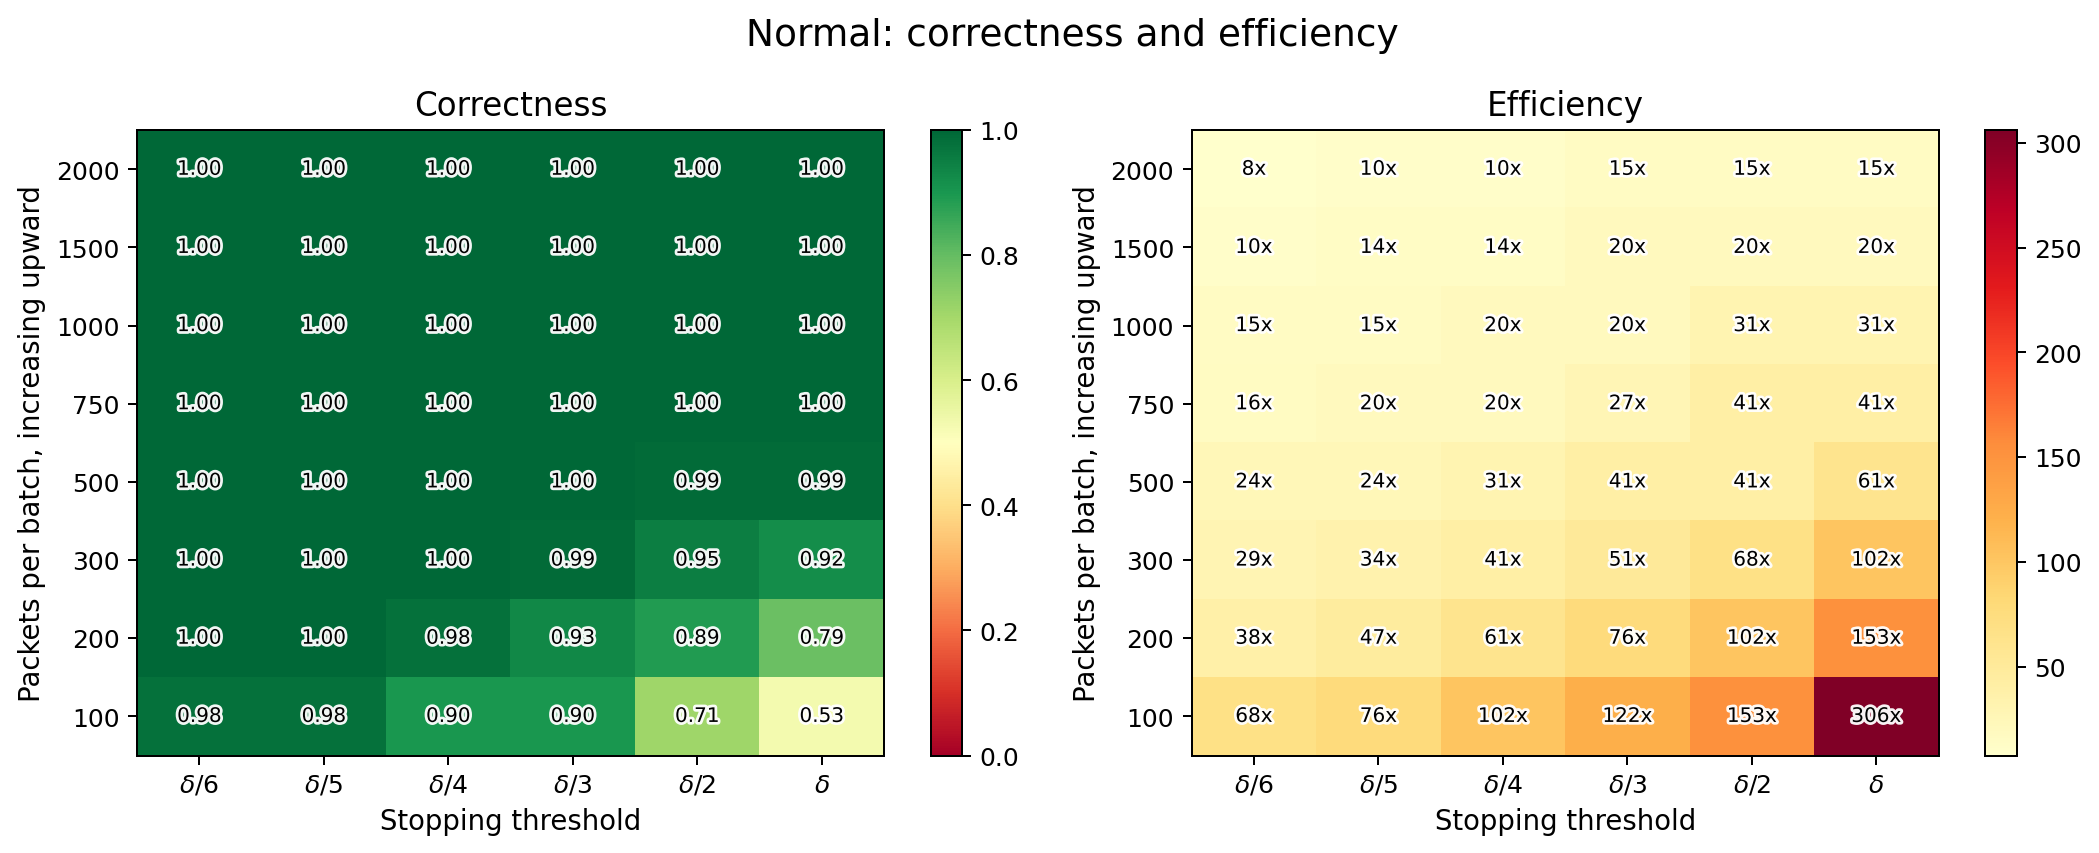
\includegraphics[width=\textwidth]{heatmap_cont_normal.png}
\caption{Correctness and efficiency for the normal distribution. The supporting heatmap shows that the conservative continuous operating point is not specific to Weibull.}
\label{fig:app-adaptive-normal-efficiency}
\end{figure}

\begin{figure}[htbp]
\centering

\includegraphics[width=\textwidth]{heatmap_cont_lognormal.png}
\caption{Correctness and efficiency for the lognormal distribution. Loose thresholds still stop too early, while \(B=200,\theta=\delta/6\) gives a reliable estimate.}
\label{fig:app-adaptive-lognormal-efficiency}
\end{figure}

\begin{figure}[htbp]
\centering
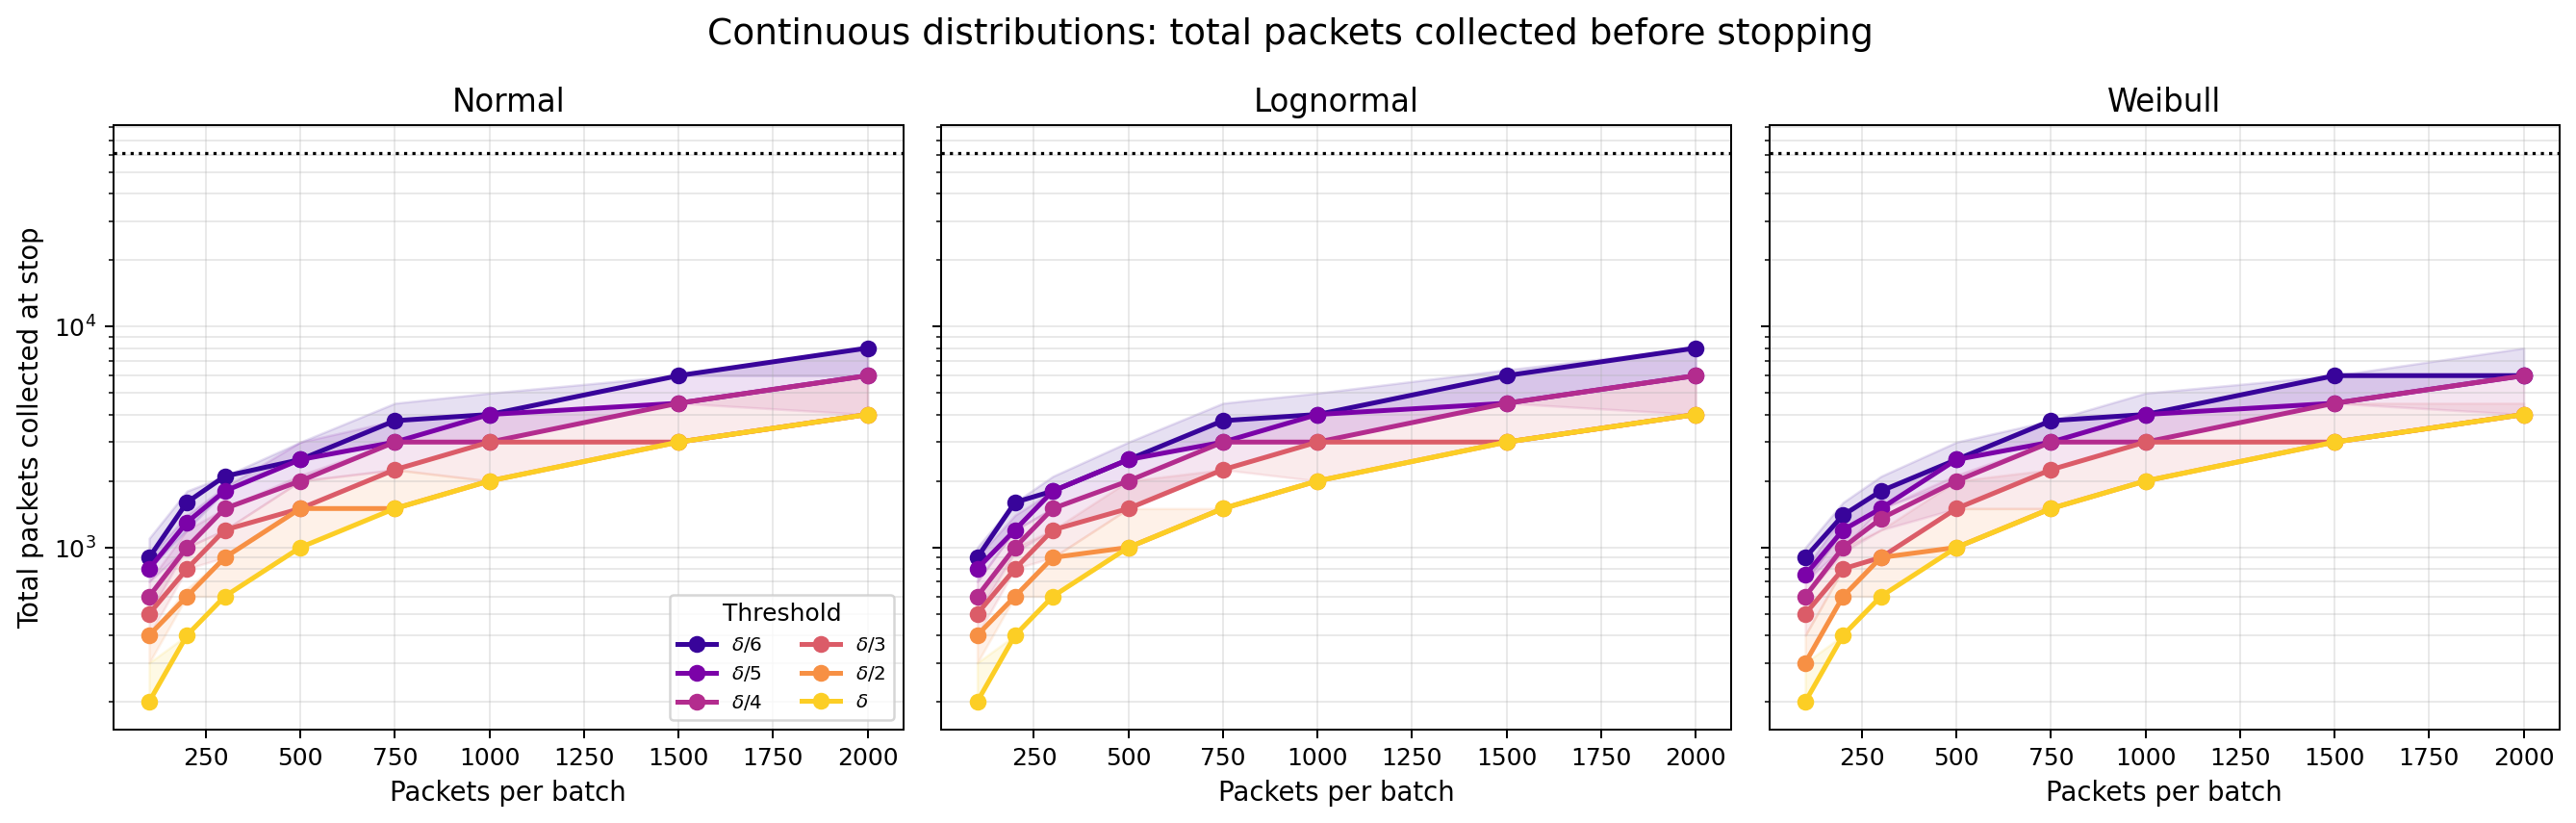
\includegraphics[width=\textwidth]{n_stop_summary_cont_all.png}
\caption{Median total packets collected before stopping for the continuous distributions. Shading shows the interquartile range across seeds, and the dotted line shows the theoretical sample bound used in the adaptive sweep.}
\label{fig:n-stop-summary-cont-all}
\end{figure}

\begin{figure}[htbp]
\centering
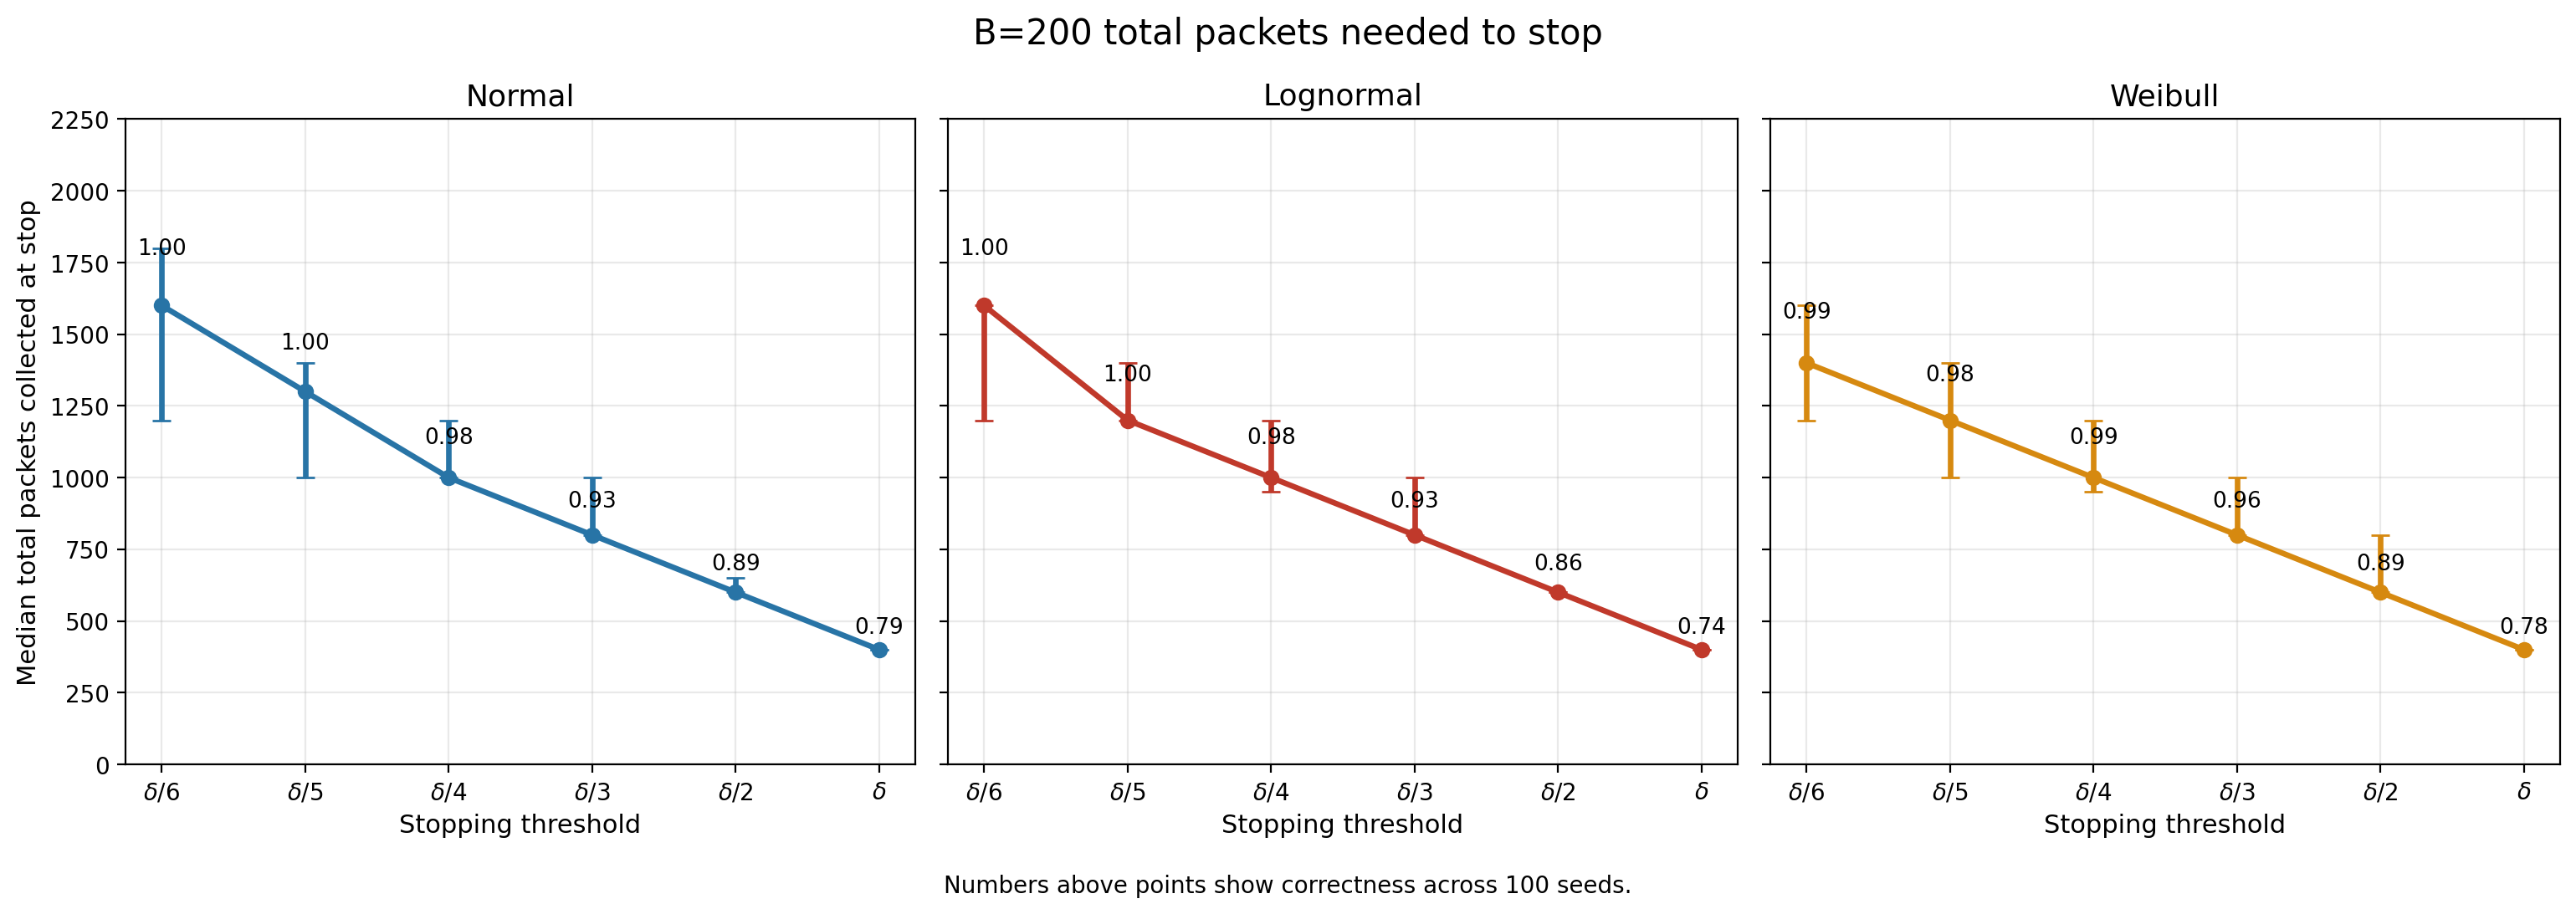
\includegraphics[width=\textwidth]{n_stop_b200_continuous.png}
\caption{Median total packets collected before stopping at \(B=200\) for the continuous distributions. Error bars show the interquartile range across seeds, and the number above each point is the correctness over 100 seeds.}
\label{fig:n-stop-b200-continuous}
\end{figure}

\begin{figure}[htbp]
\centering
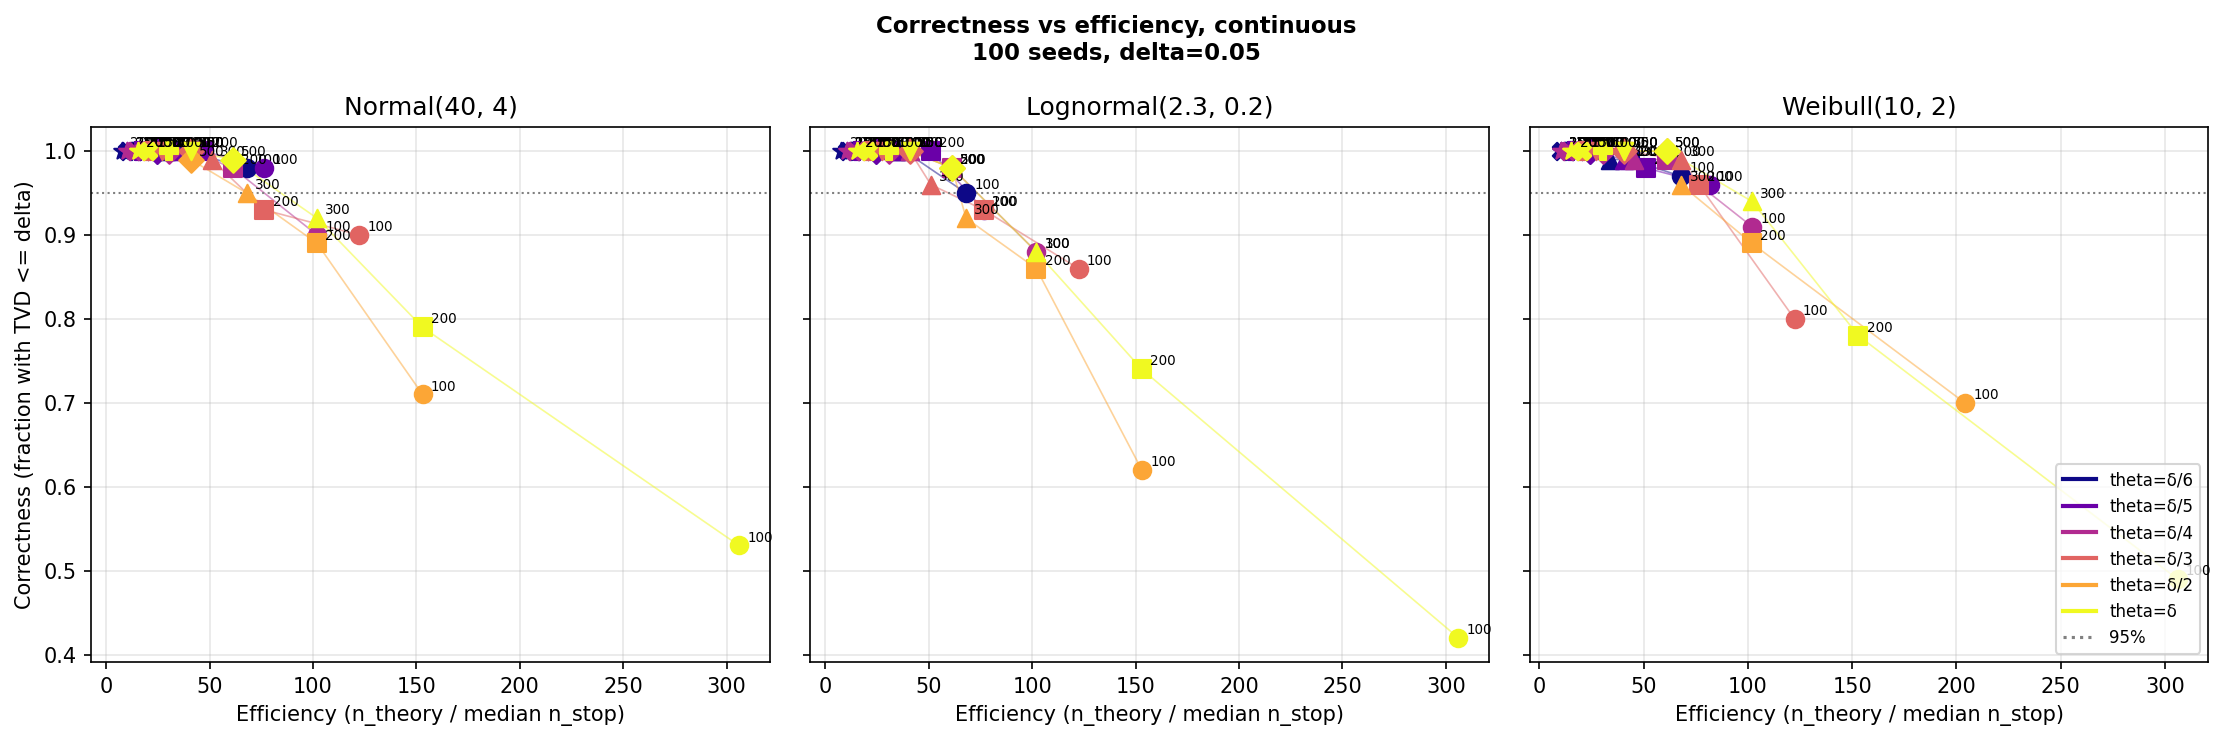
\includegraphics[width=\textwidth]{scatter_cont.png}
\caption{Continuous correctness against efficiency. Each point is one stopping configuration.}
\label{fig:app-scatter-cont}
\end{figure}

\begin{figure}[htbp]
\centering
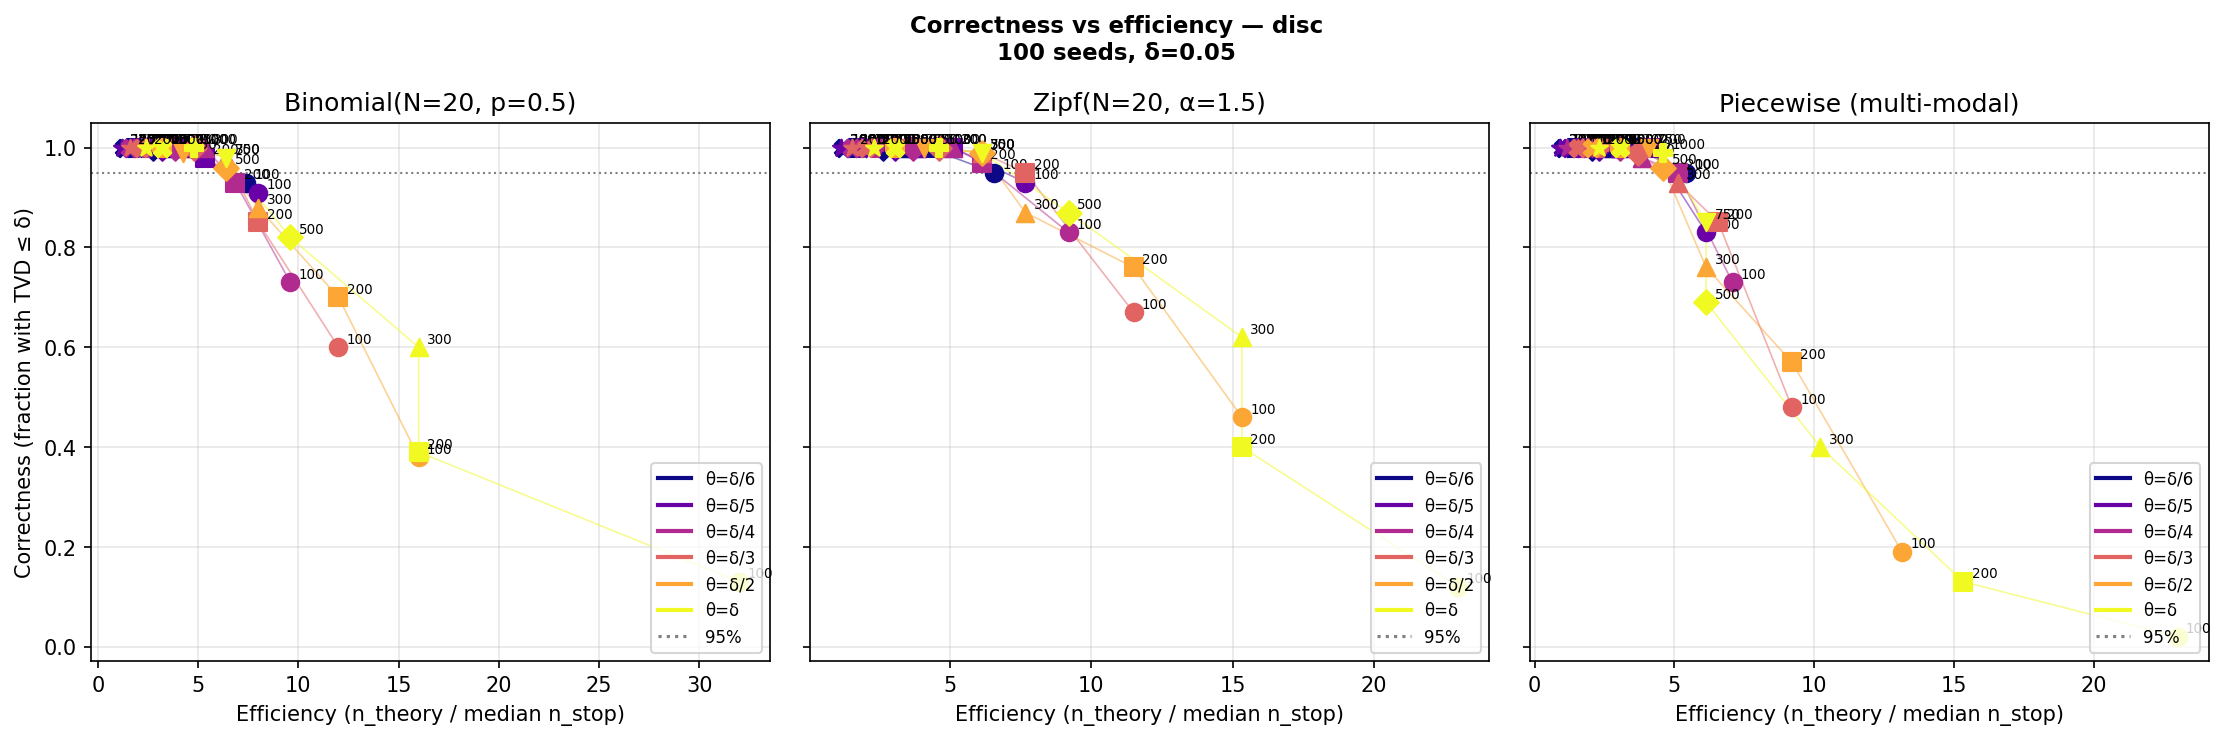
\includegraphics[width=\textwidth]{scatter_disc.png}
\caption{Discrete correctness against efficiency. The safe region is further left than in the continuous plot.}
\label{fig:app-scatter-disc}
\end{figure}

\begin{figure}[htbp]
\centering
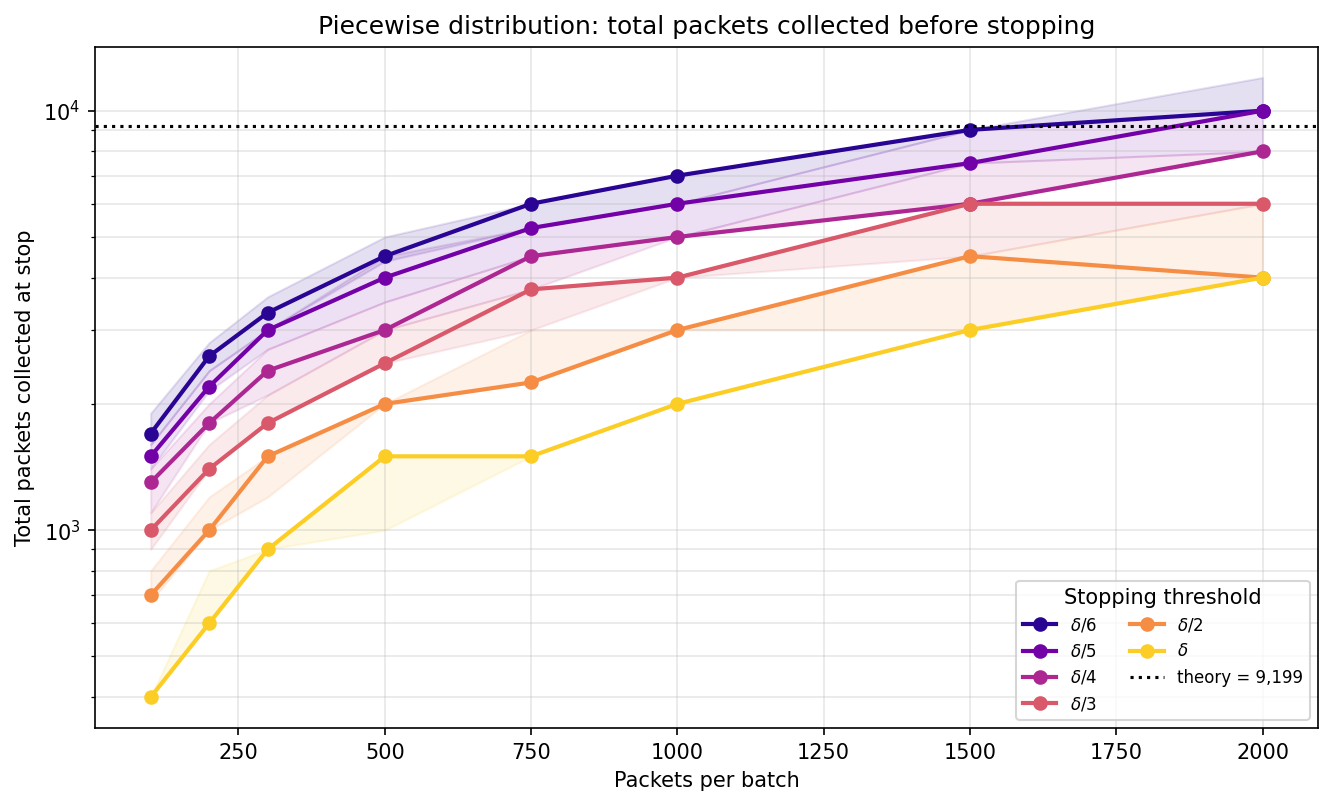
\includegraphics[width=0.92\textwidth]{n_stop_summary_disc_piecewise.png}
\caption{Median total packets collected before stopping for the piecewise distribution.}
\label{fig:app-n-stop-piecewise}
\end{figure}

\begin{figure}[htbp]
\centering
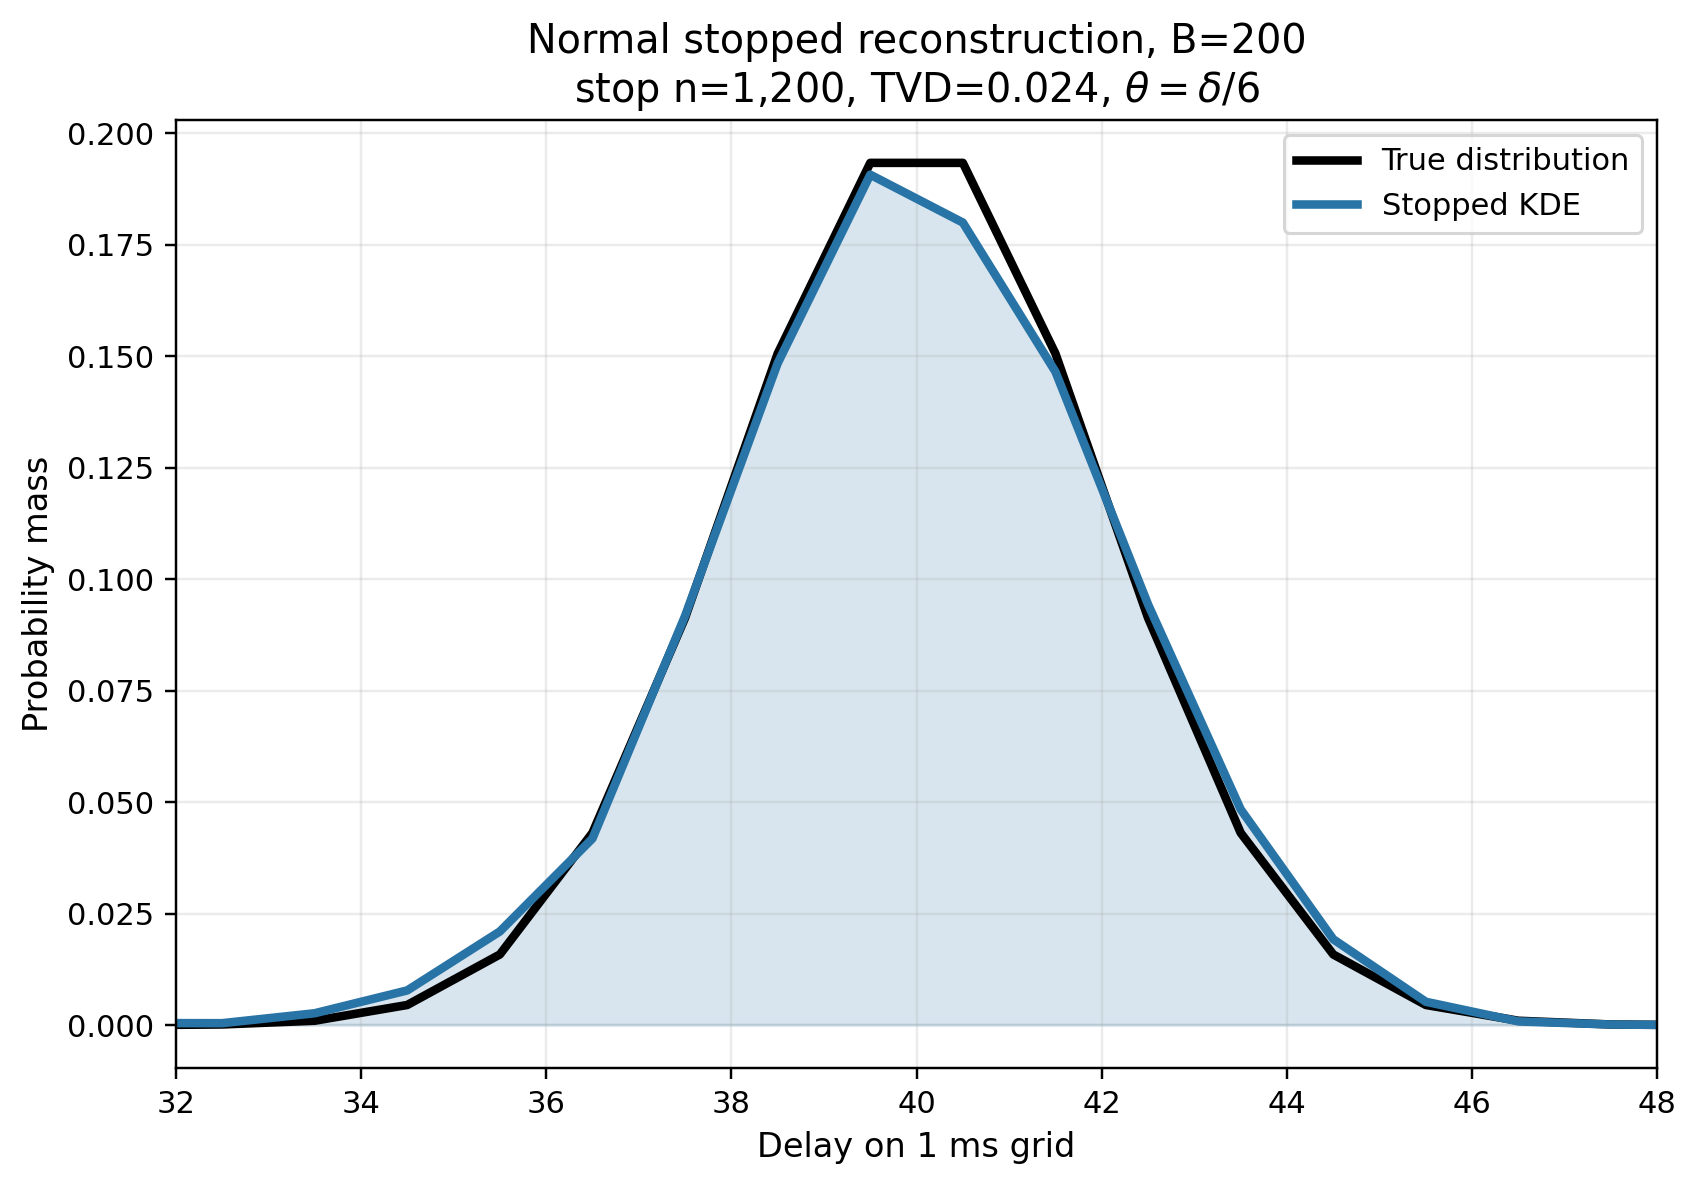
\includegraphics[width=0.92\textwidth]{stopped_distribution_normal_b200.png}
\caption{Stopped KDE reconstruction for the normal distribution at \(B=200\) and \(\theta=\delta/6\). The centre and tails are already close to the true distribution at the stopping point.}
\label{fig:app-stopped-distribution-normal-b200}
\end{figure}

\begin{figure}[htbp]
\centering
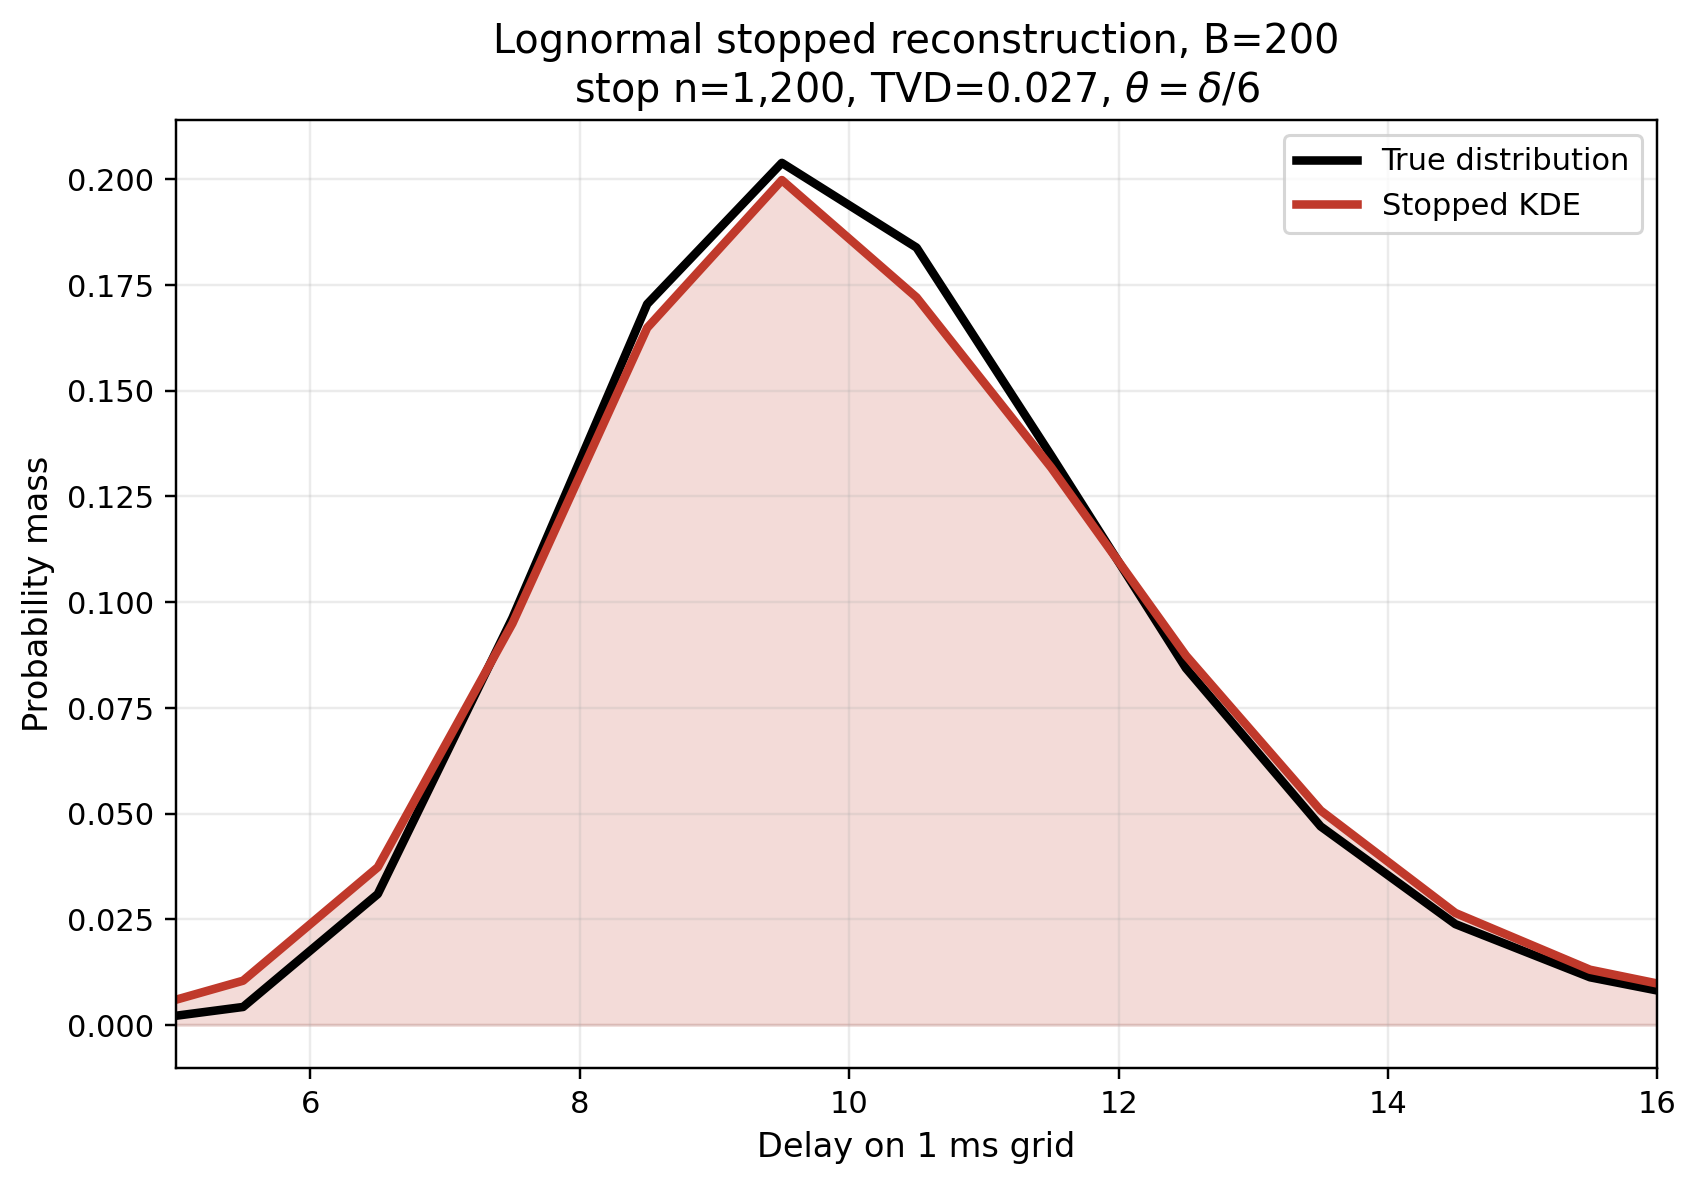
\includegraphics[width=0.92\textwidth]{stopped_distribution_lognormal_b200.png}
\caption{Stopped KDE reconstruction for the lognormal distribution at \(B=200\) and \(\theta=\delta/6\). The estimate preserves the right-skewed shape used by the later distributional comparison.}
\label{fig:app-stopped-distribution-lognormal-b200}
\end{figure}

\begin{figure}[htbp]
\centering
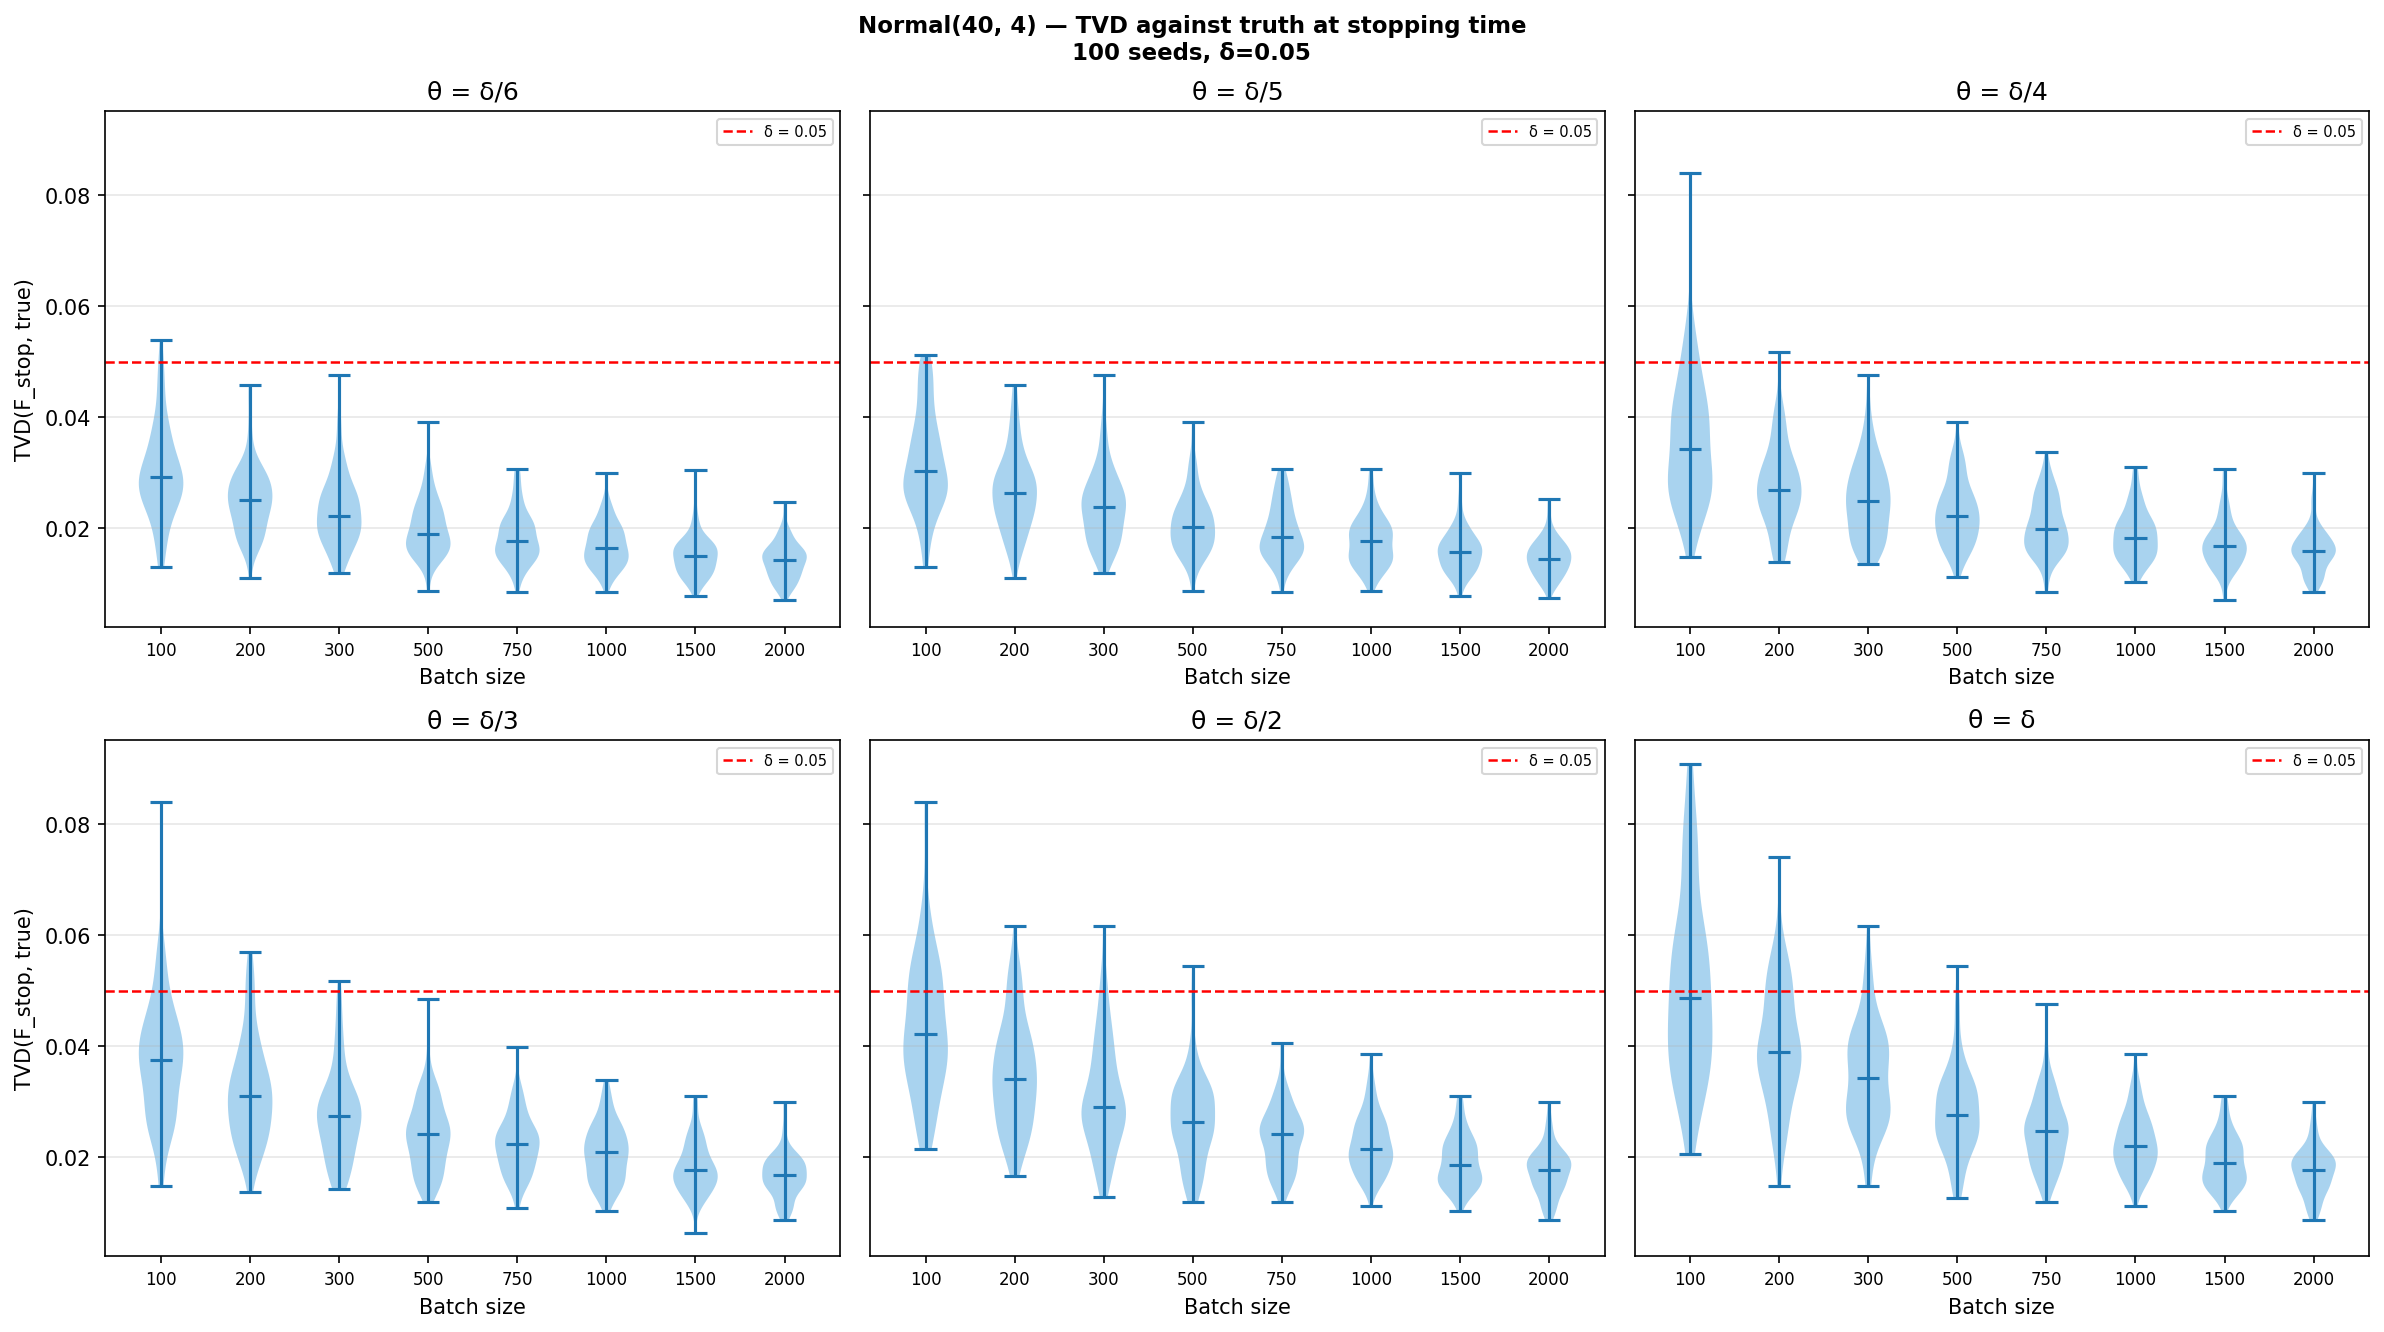
\includegraphics[width=\textwidth]{tvd_at_stop_cont_normal.png}
\caption{Distribution of TVD against truth at the stopping time for the normal distribution.}
\label{fig:app-tvd-stop-normal}
\end{figure}

\begin{figure}[htbp]
\centering
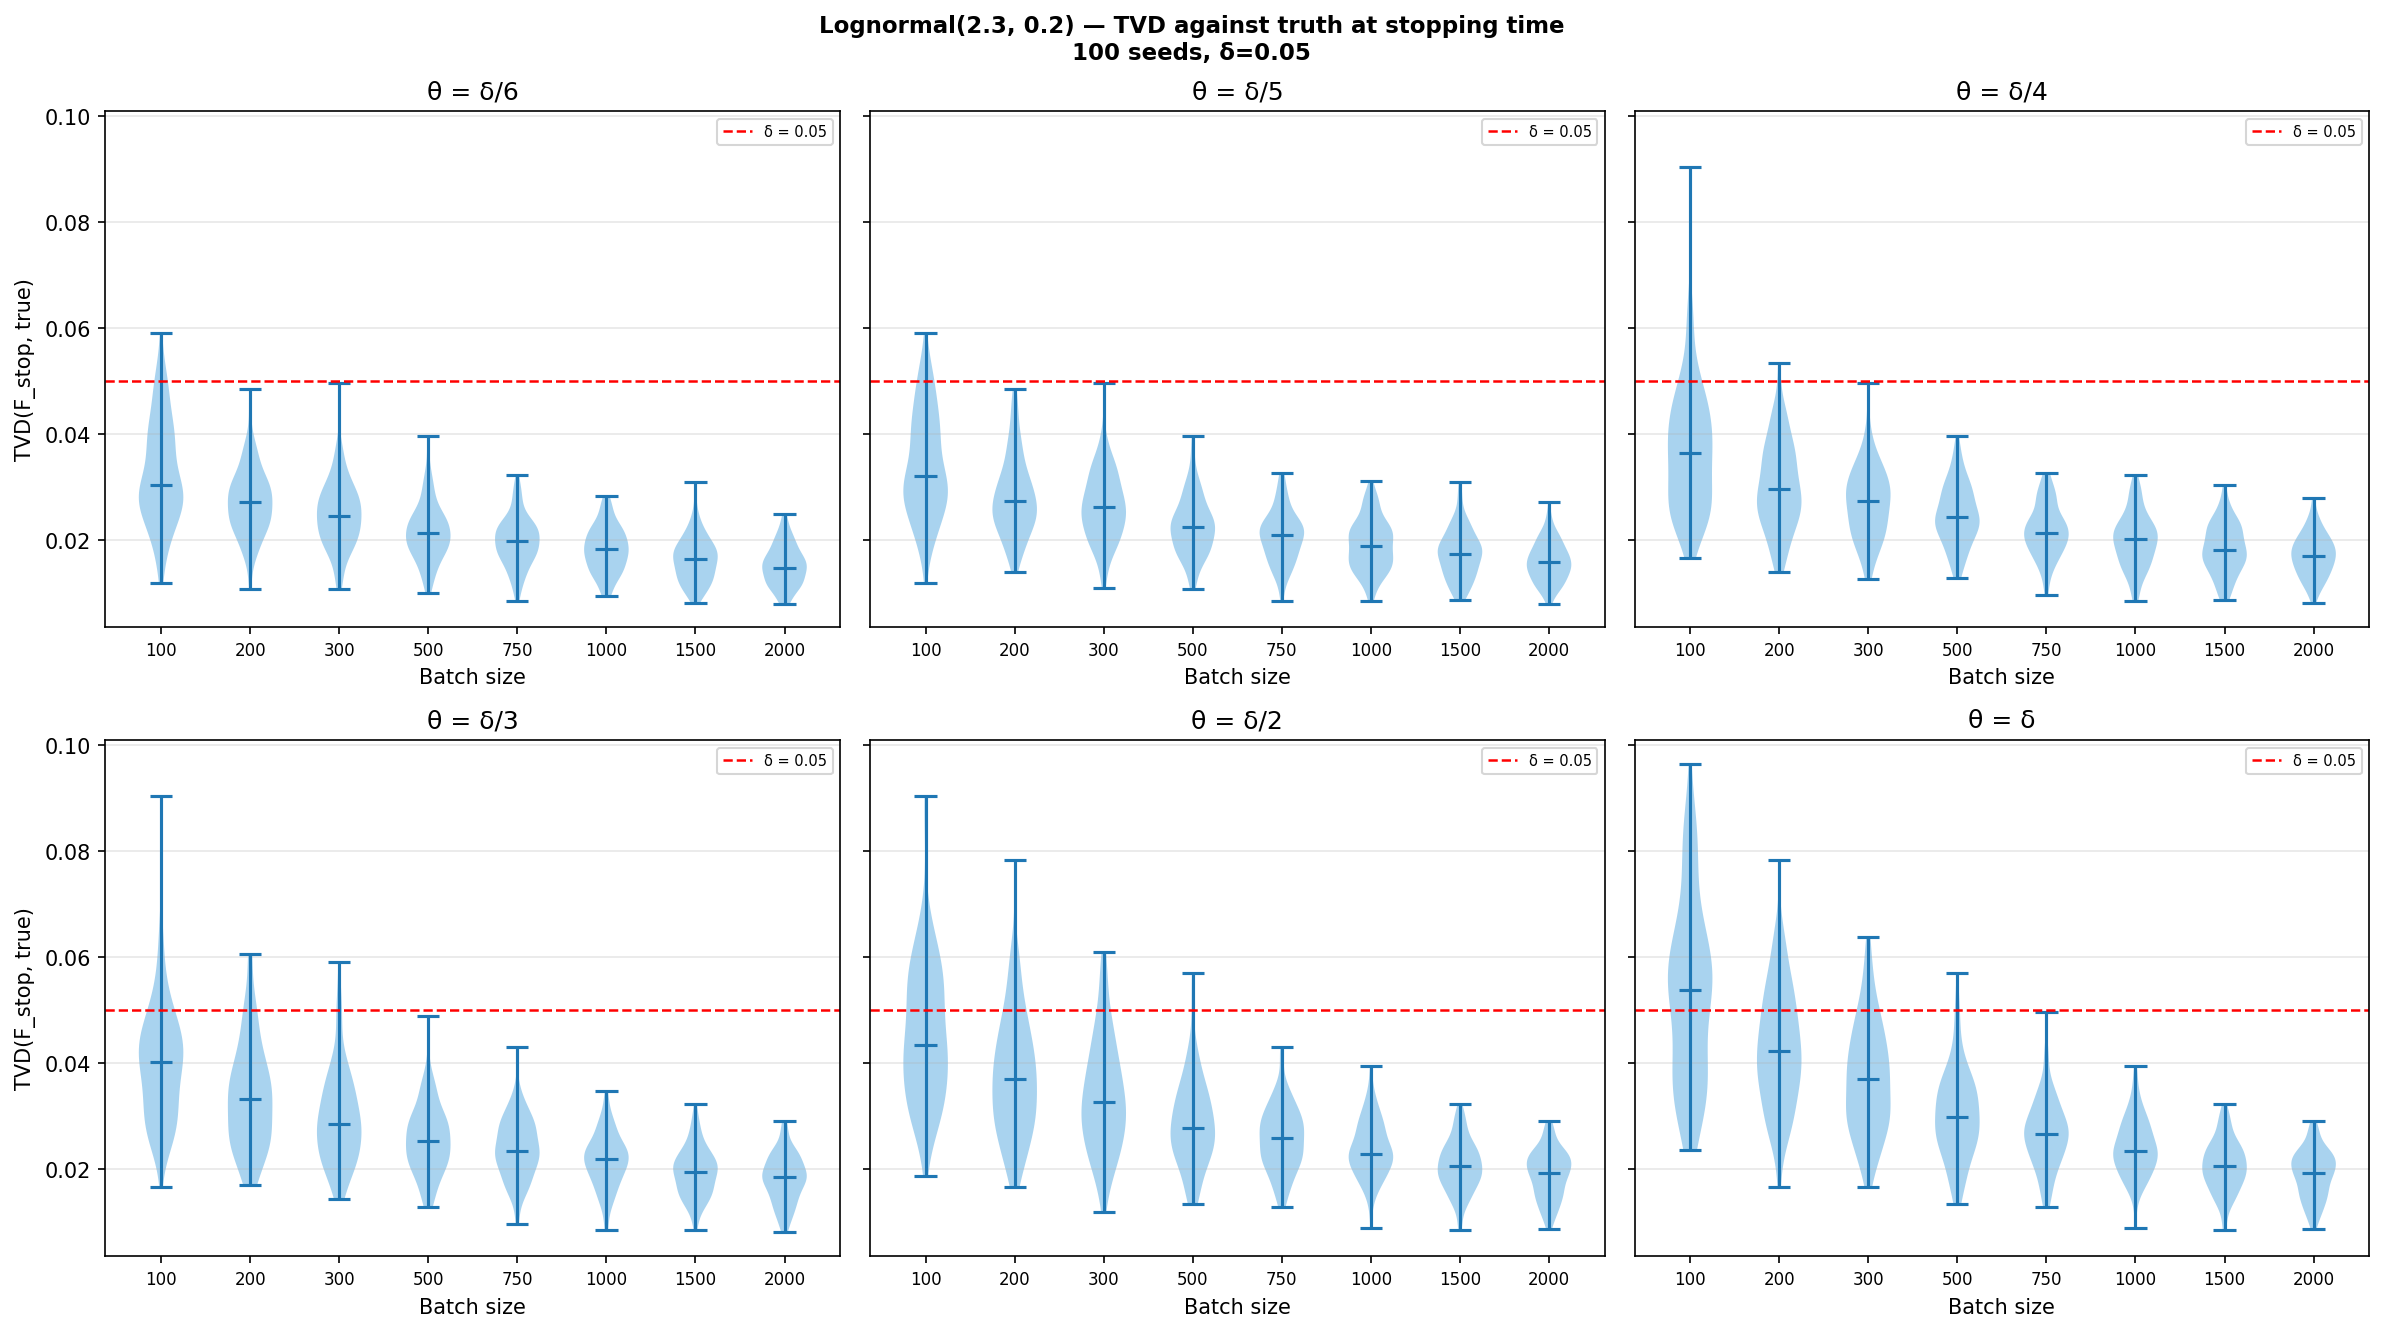
\includegraphics[width=\textwidth]{tvd_at_stop_cont_lognormal.png}
\caption{Distribution of TVD against truth at the stopping time for the lognormal distribution.}
\label{fig:app-tvd-stop-lognormal}
\end{figure}

\begin{figure}[htbp]
\centering
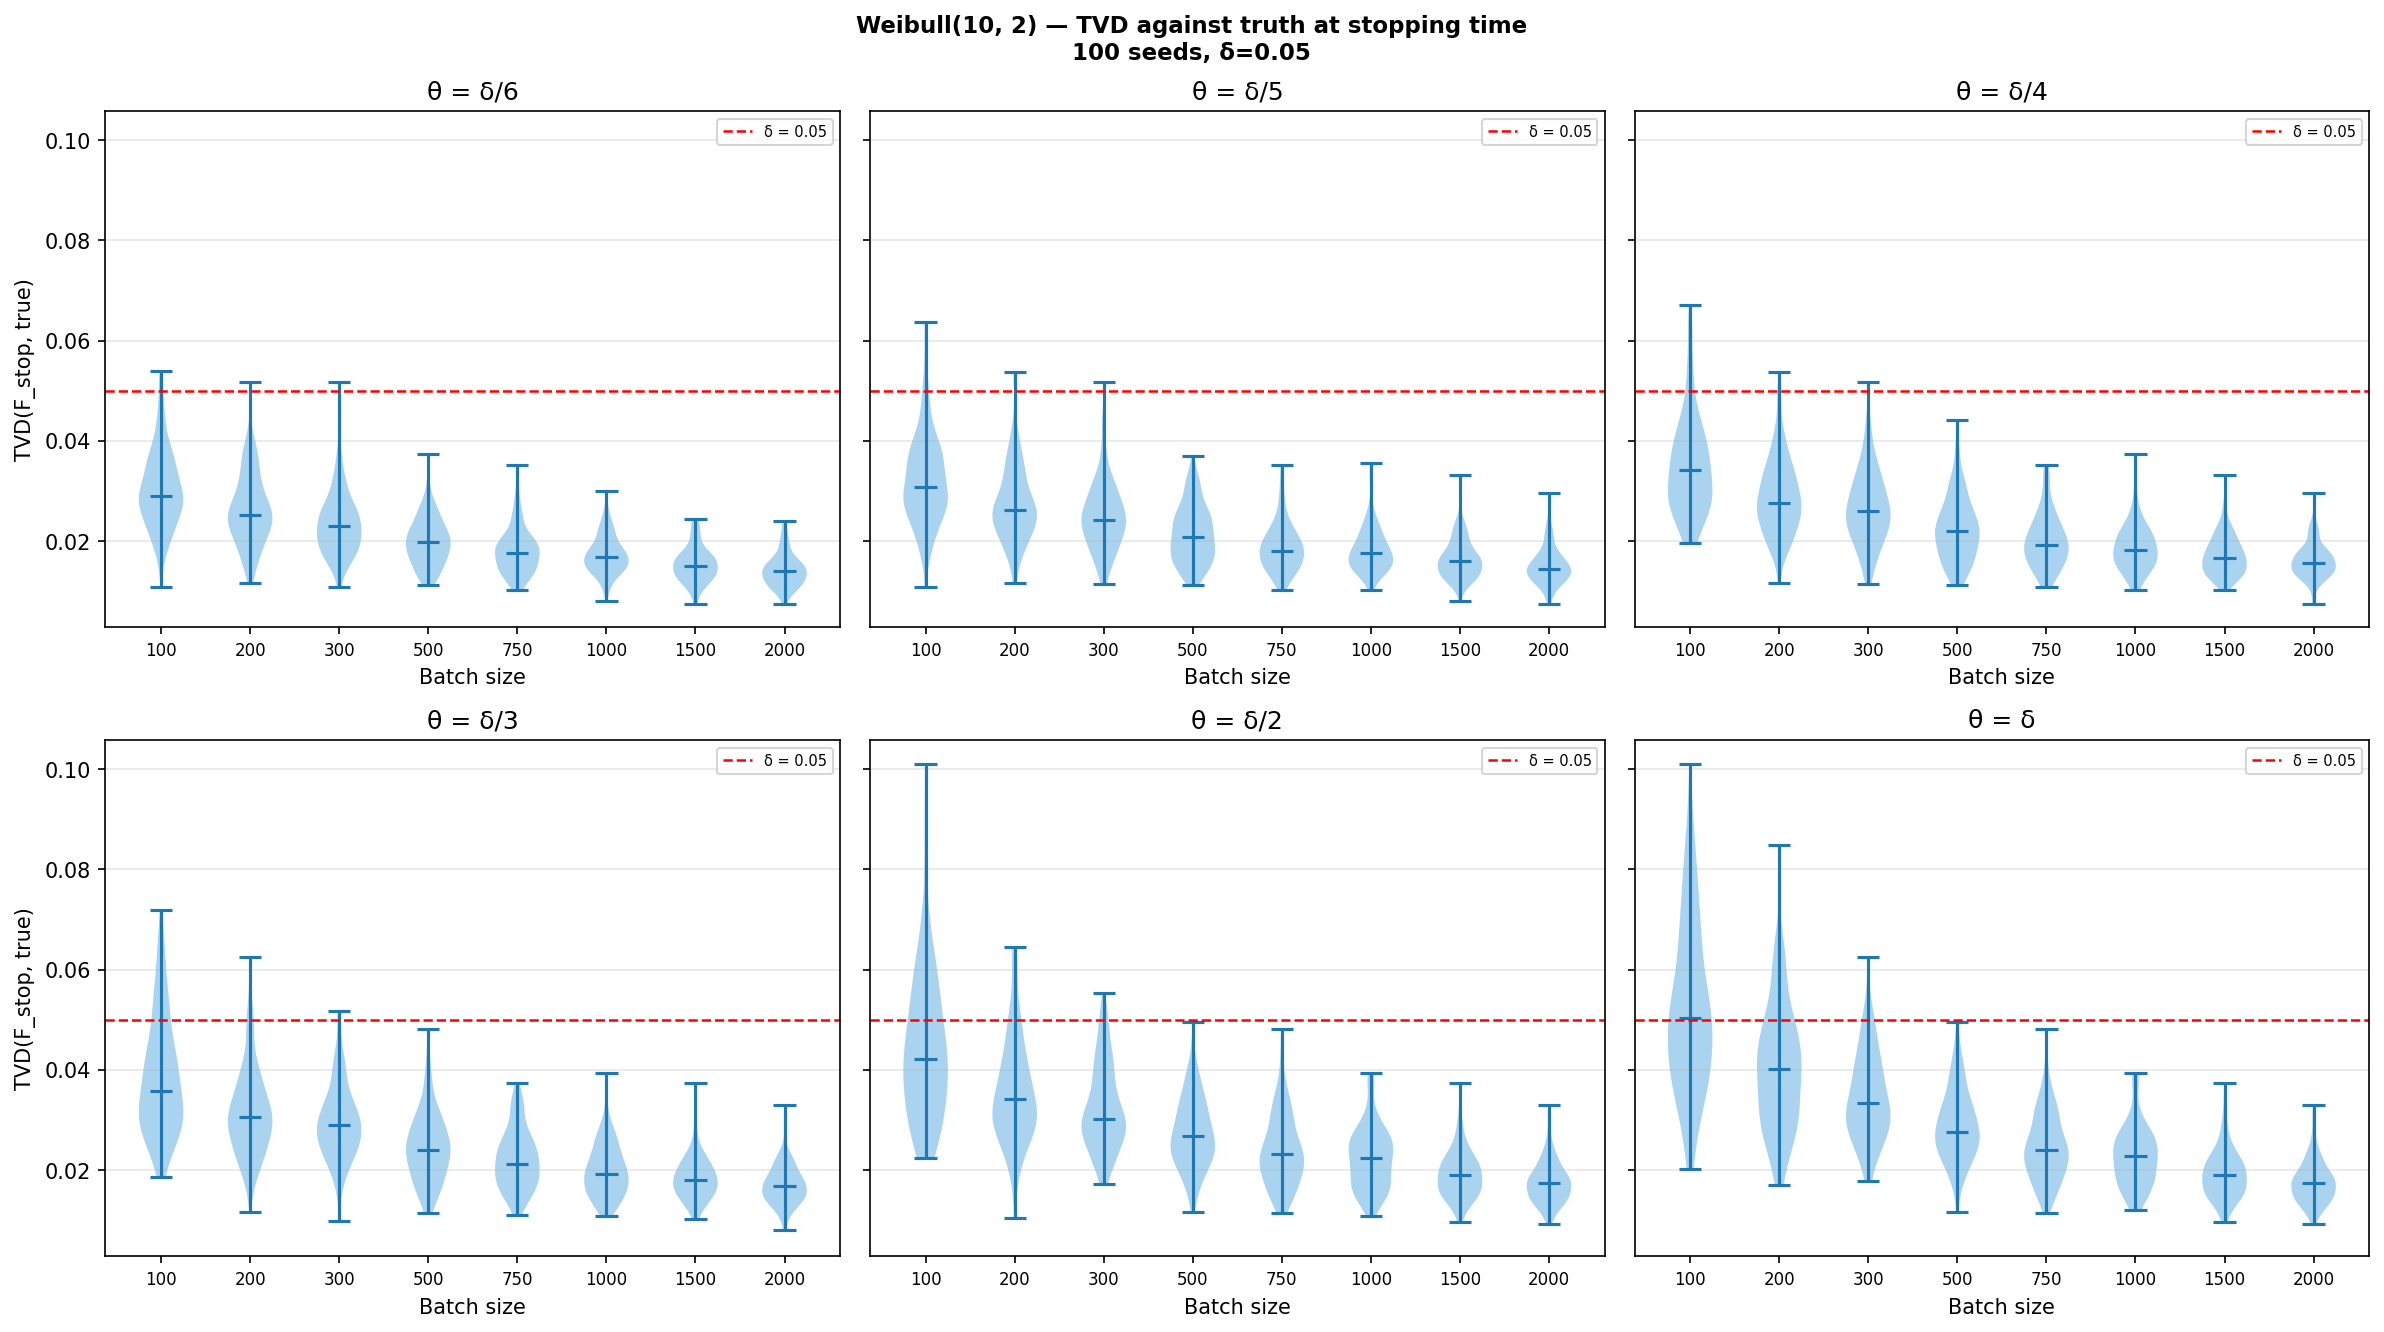
\includegraphics[width=\textwidth]{tvd_at_stop_cont_weibull.png}
\caption{Distribution of TVD against truth at the stopping time for the Weibull distribution.}
\label{fig:app-tvd-stop-weibull}
\end{figure}

\begin{figure}[htbp]
\centering
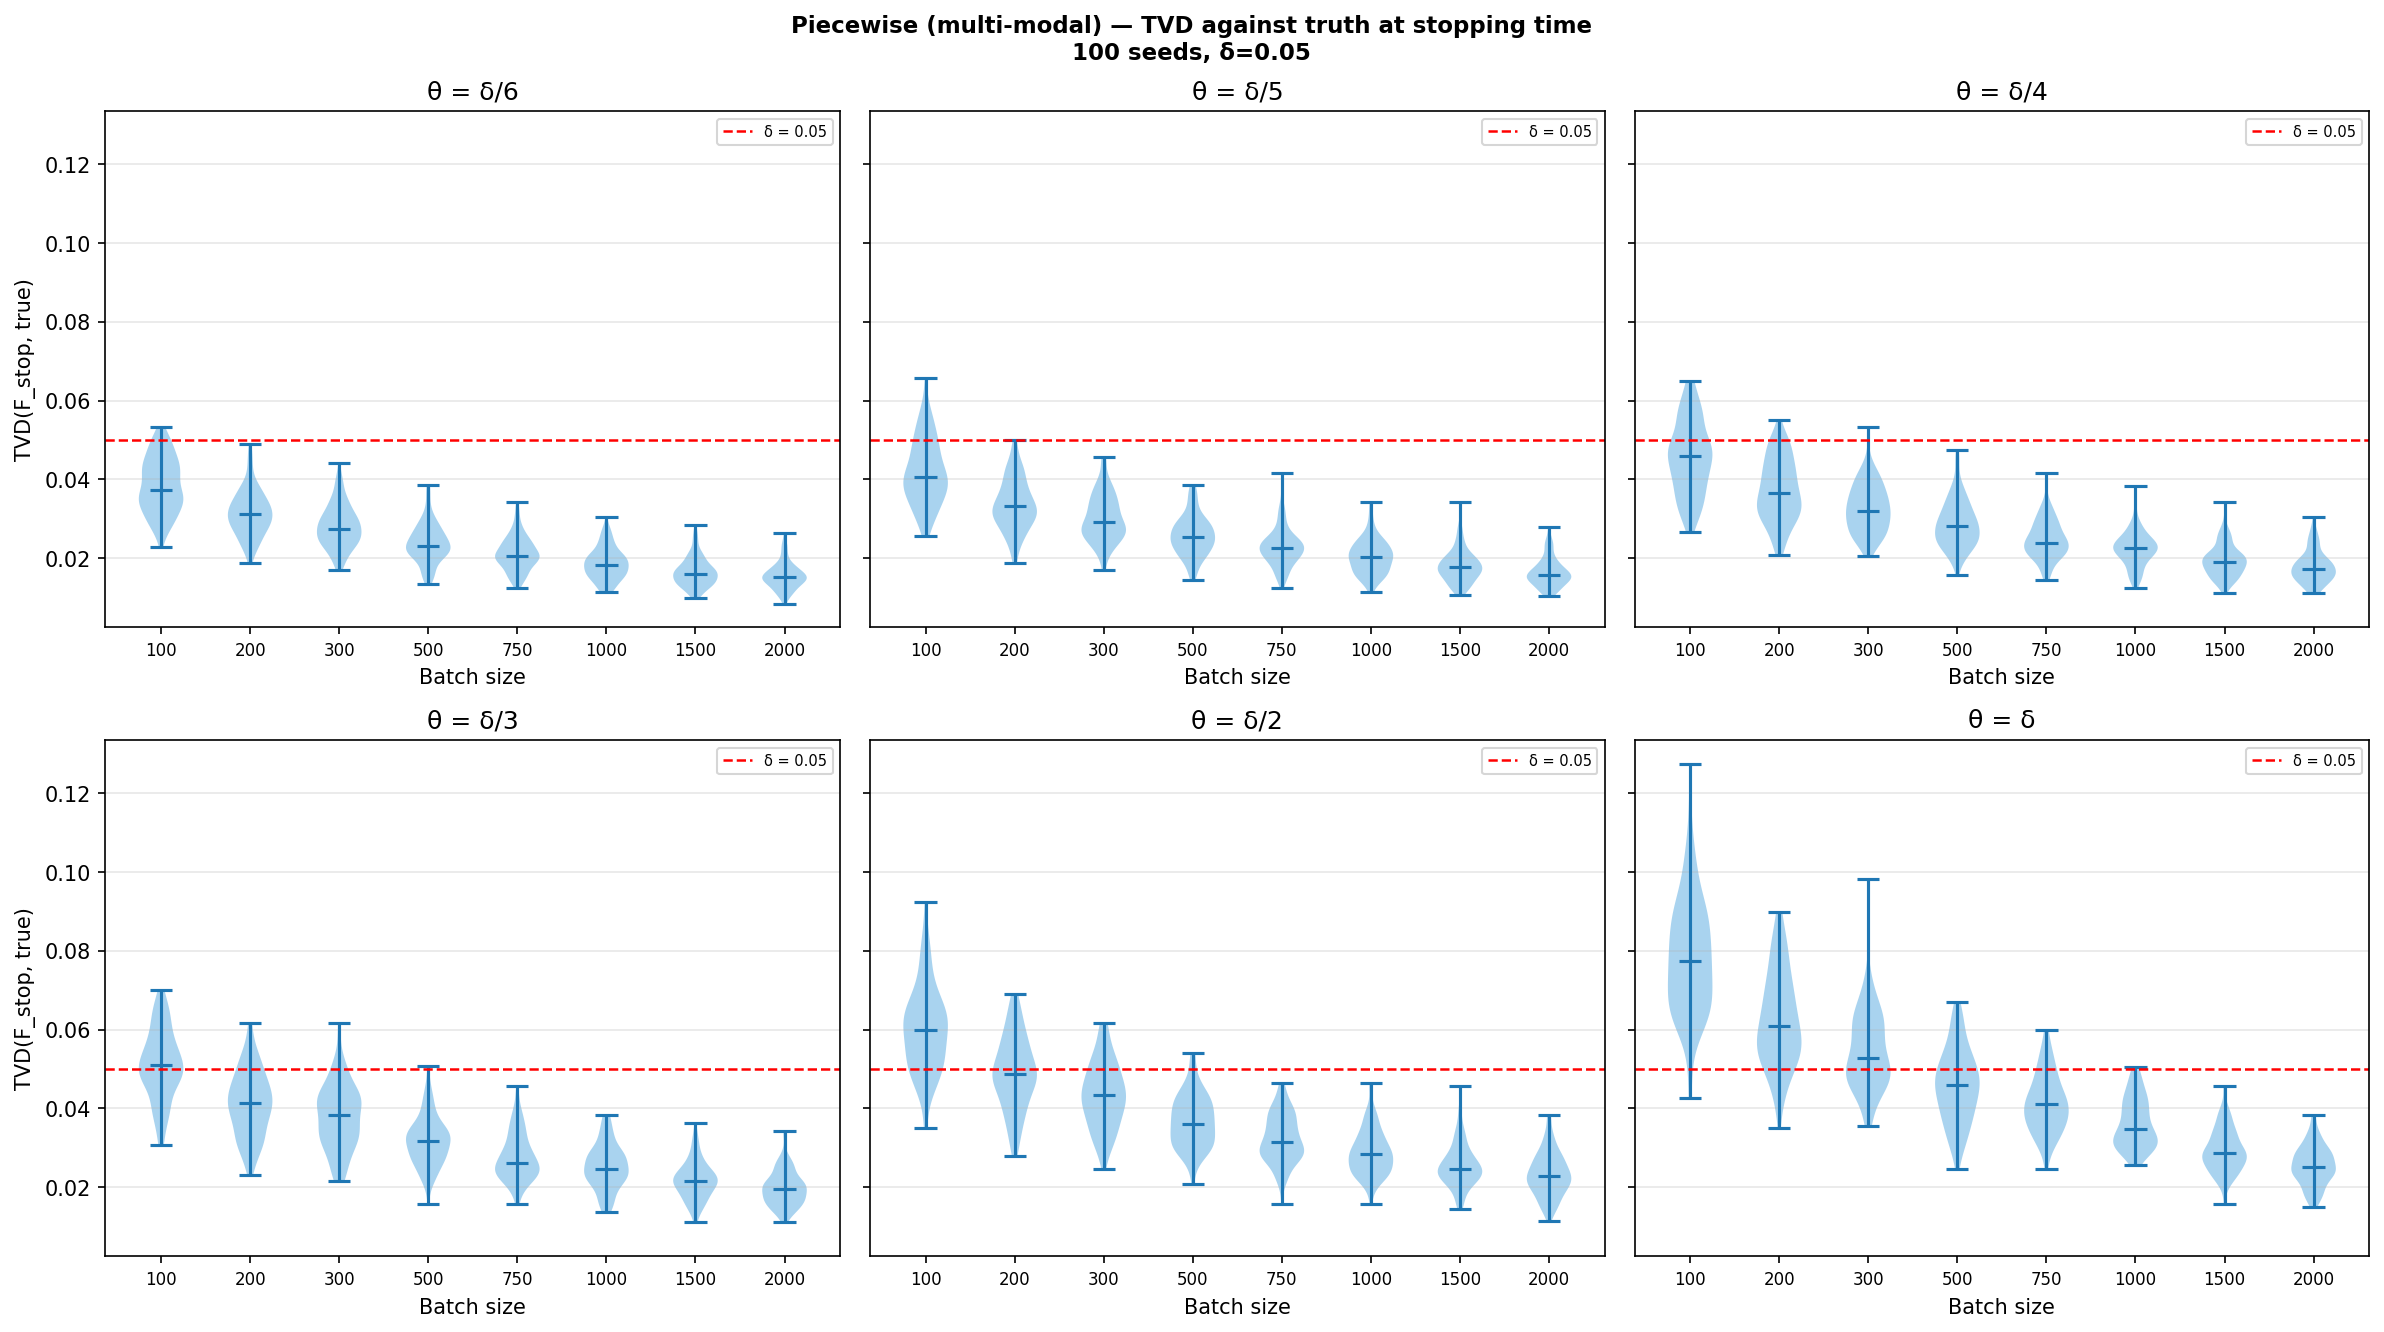
\includegraphics[width=\textwidth]{tvd_at_stop_disc_piecewise.png}
\caption{Distribution of TVD against truth at the stopping time for the piecewise distribution.}
\label{fig:app-tvd-stop-piecewise}
\end{figure}

\clearpage

\section{Capacity use-case diagnostics}
\label{app:capacity-use-case-diagnostics}

\begin{figure}[htbp]
\centering
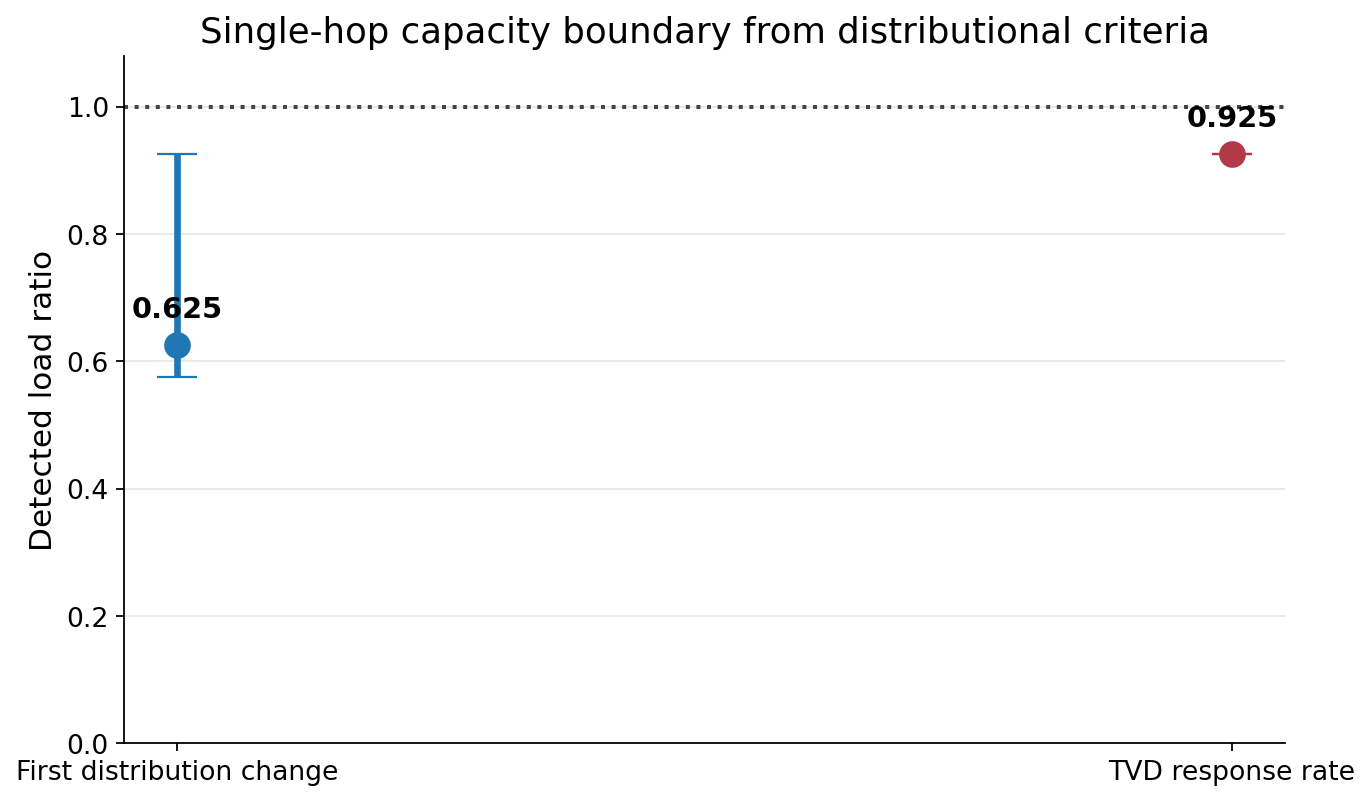
\includegraphics[width=\textwidth]{observable_capacity_single_methods.png}
\caption{Single-hop detection load for the two distributional capacity criteria. The configured capacity is used only for post-hoc evaluation.}
\label{fig:observable-single-methods}
\end{figure}

\begin{figure}[htbp]
\centering
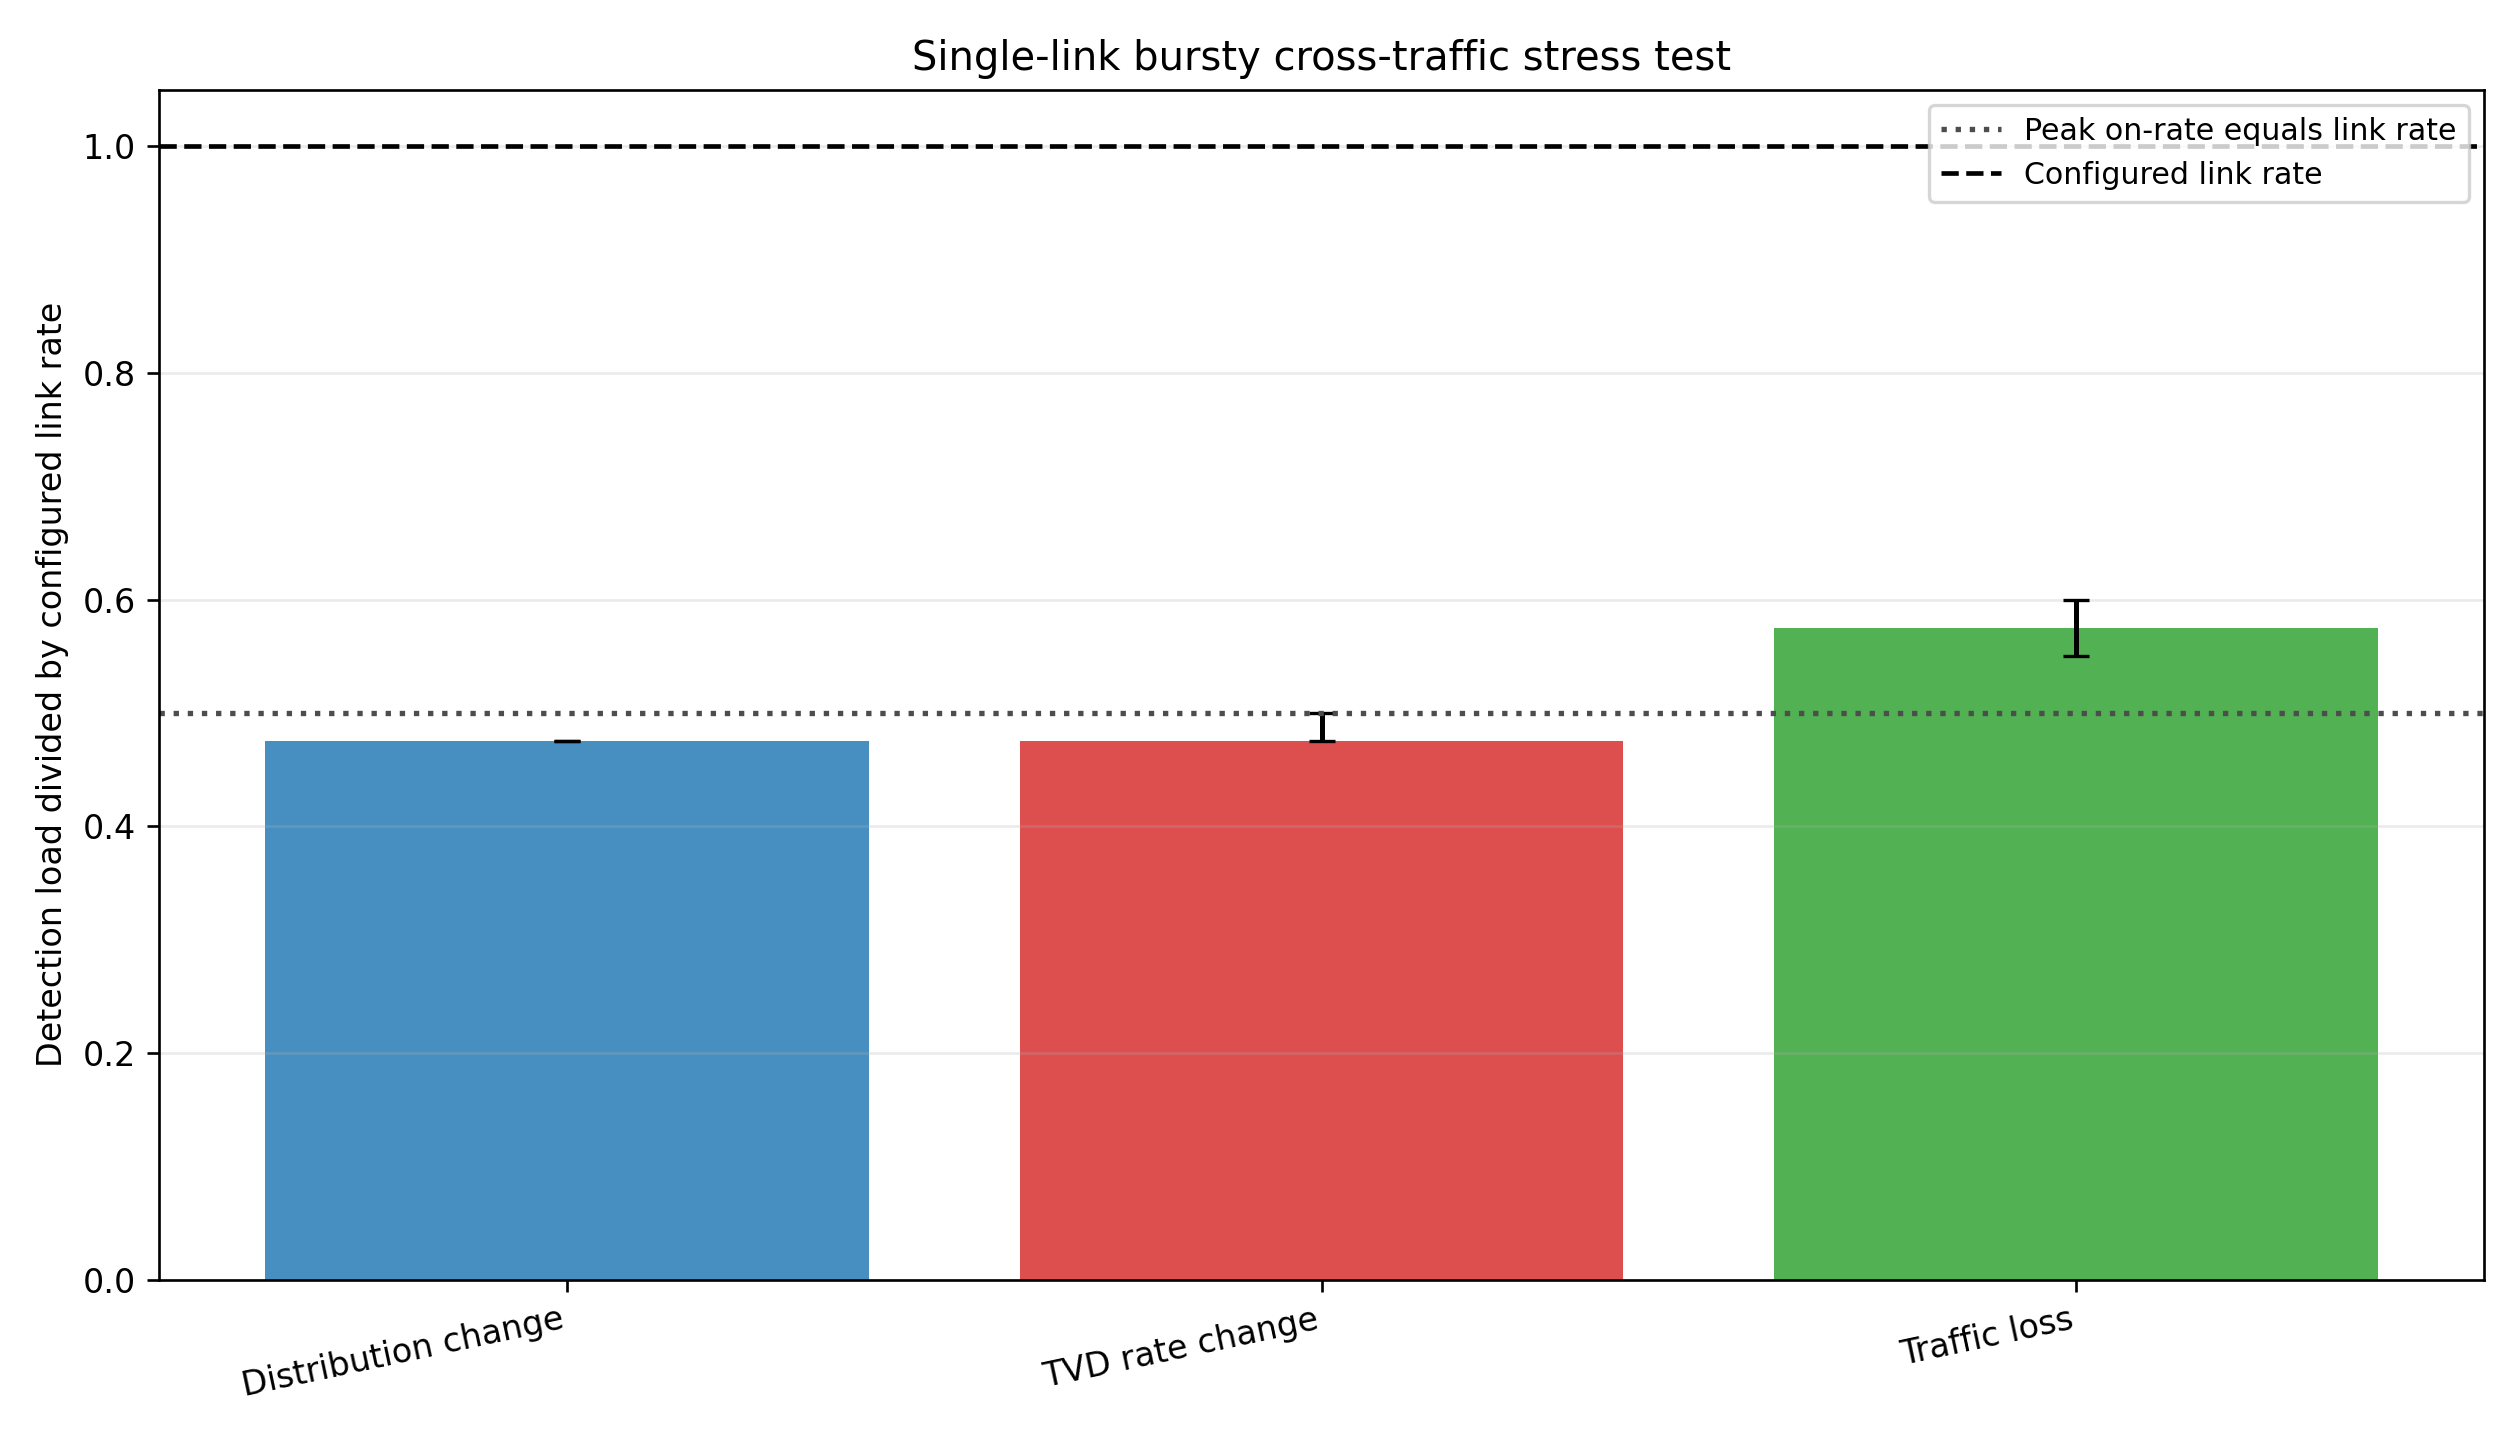
\includegraphics[width=\textwidth]{observable_capacity_bursty_methods.png}
\caption{Single-link detection load under Pareto on-off bursty cross traffic. The reported load ratio is the swept average rate, while the on-period sending rate is twice that value.}
\label{fig:observable-bursty-methods}
\end{figure}

\begin{figure}[htbp]
\centering
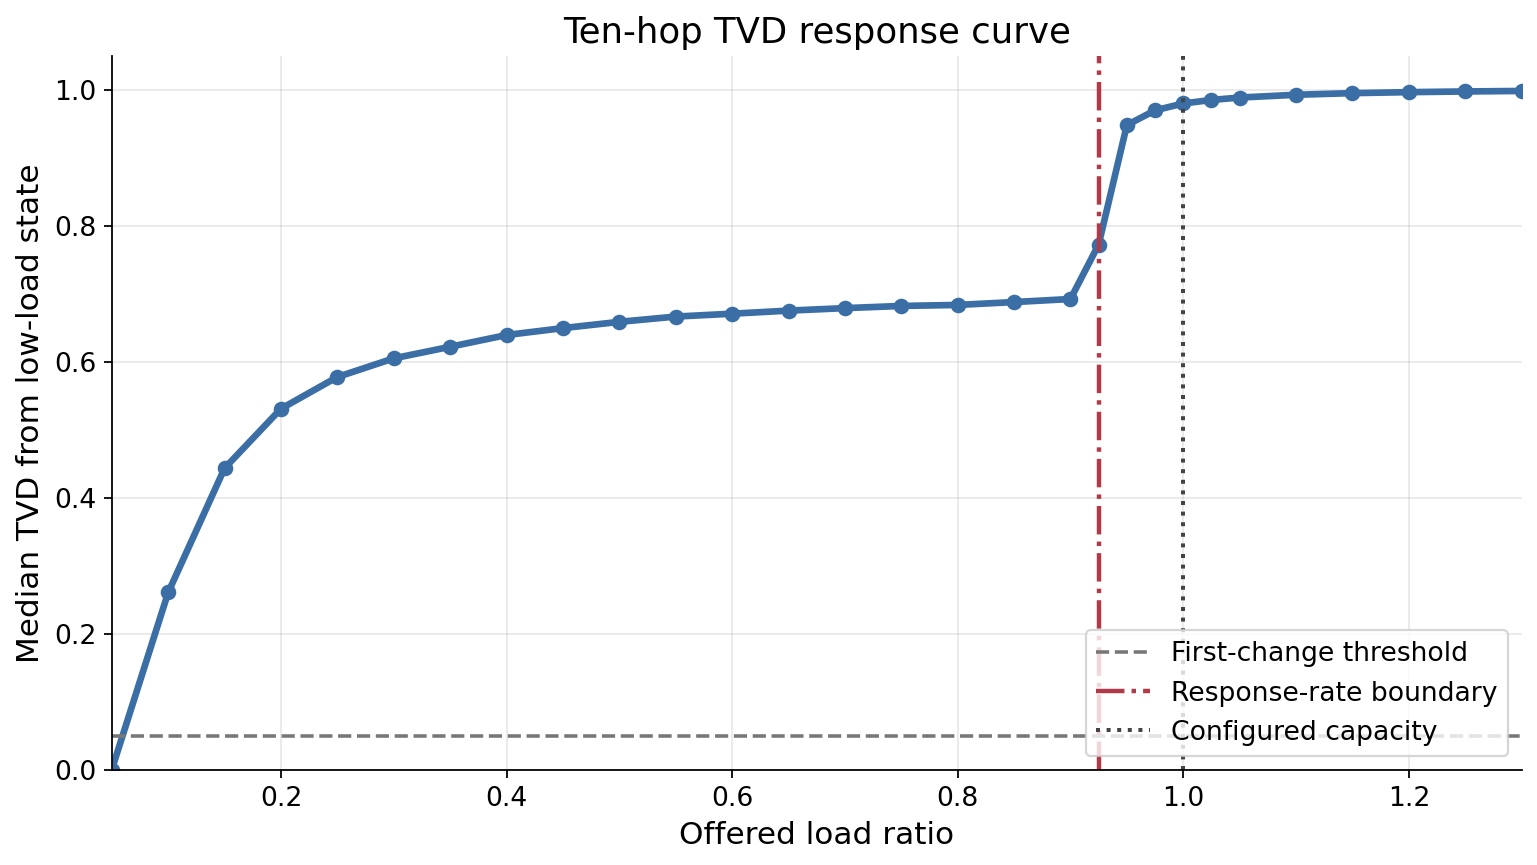
\includegraphics[width=\textwidth]{observable_capacity_multi_tvd_response.png}
\caption{TVD response for the ten-hop path-wide cross-traffic experiment. The response-rate boundary appears where the curve leaves its gradual low-load trend.}
\label{fig:app-observable-multi-tvd-response}
\end{figure}

\begin{figure}[htbp]
\centering
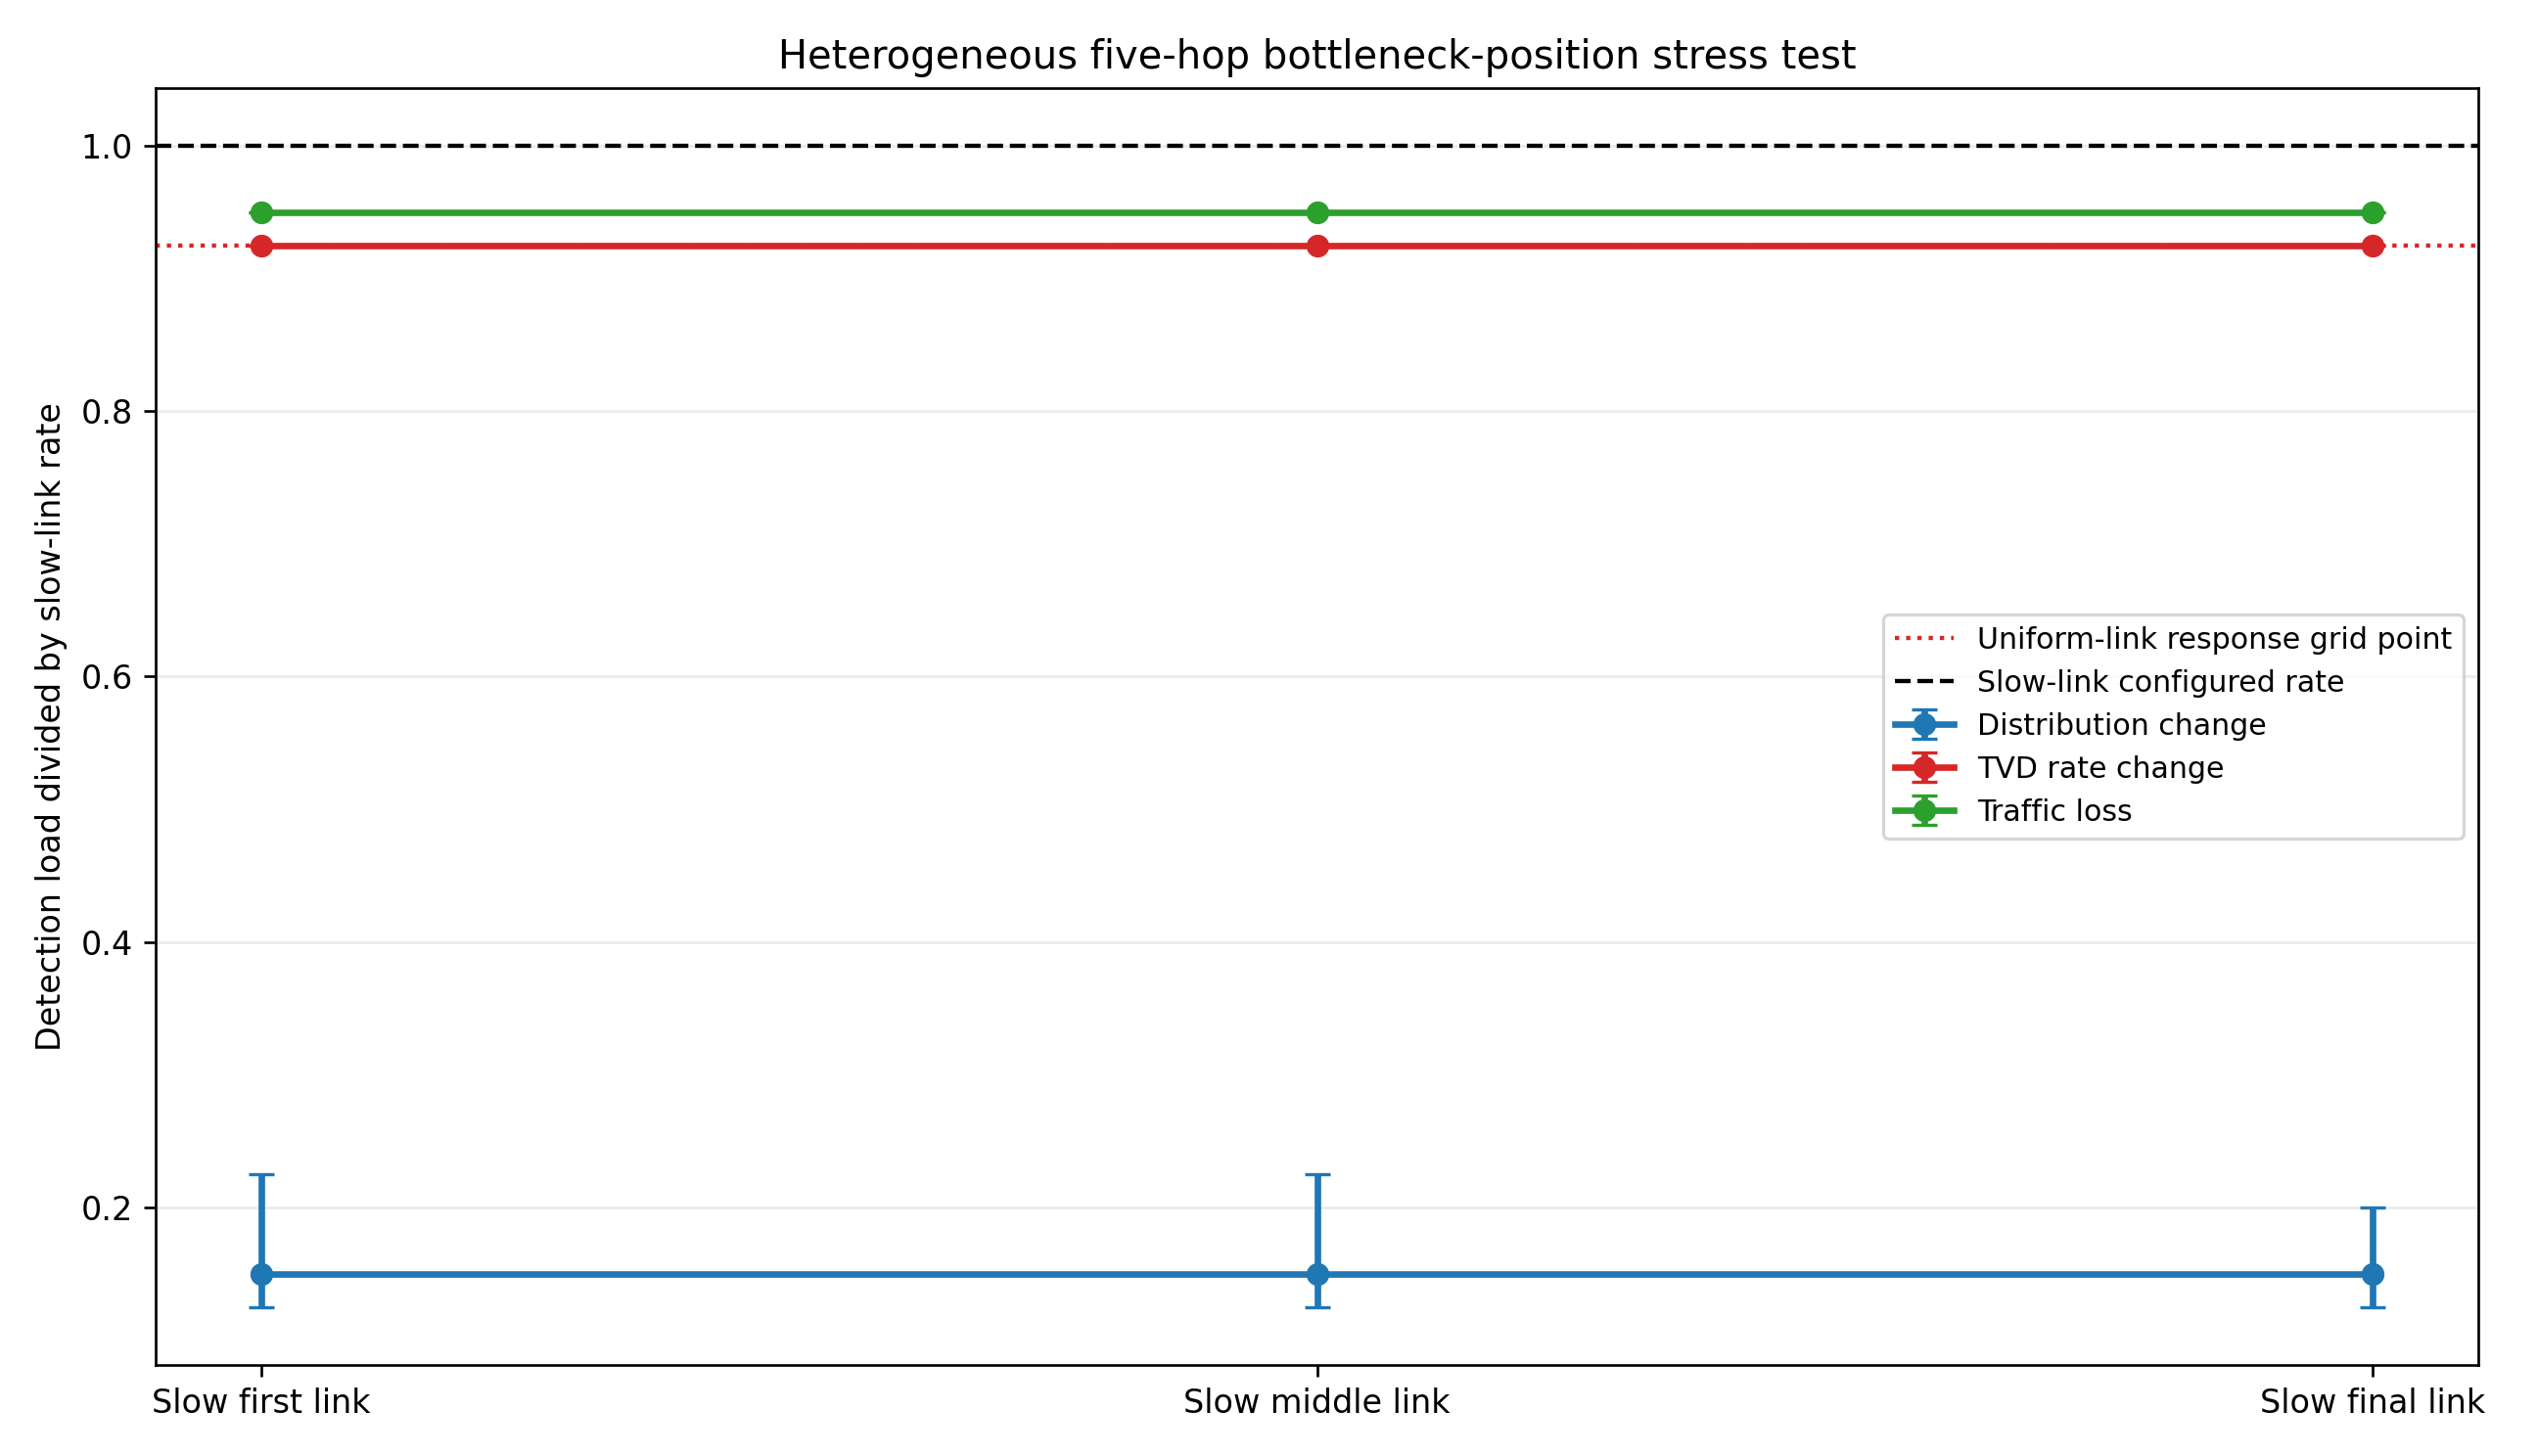
\includegraphics[width=\textwidth]{observable_capacity_heterogeneous_methods.png}
\caption{Detection load in the heterogeneous five-hop stress test. One link is 10 Mbit/s, the other four are 20 Mbit/s, and the slow link is moved across the path.}
\label{fig:observable-heterogeneous-methods}
\end{figure}

\begin{figure}[htbp]
\centering
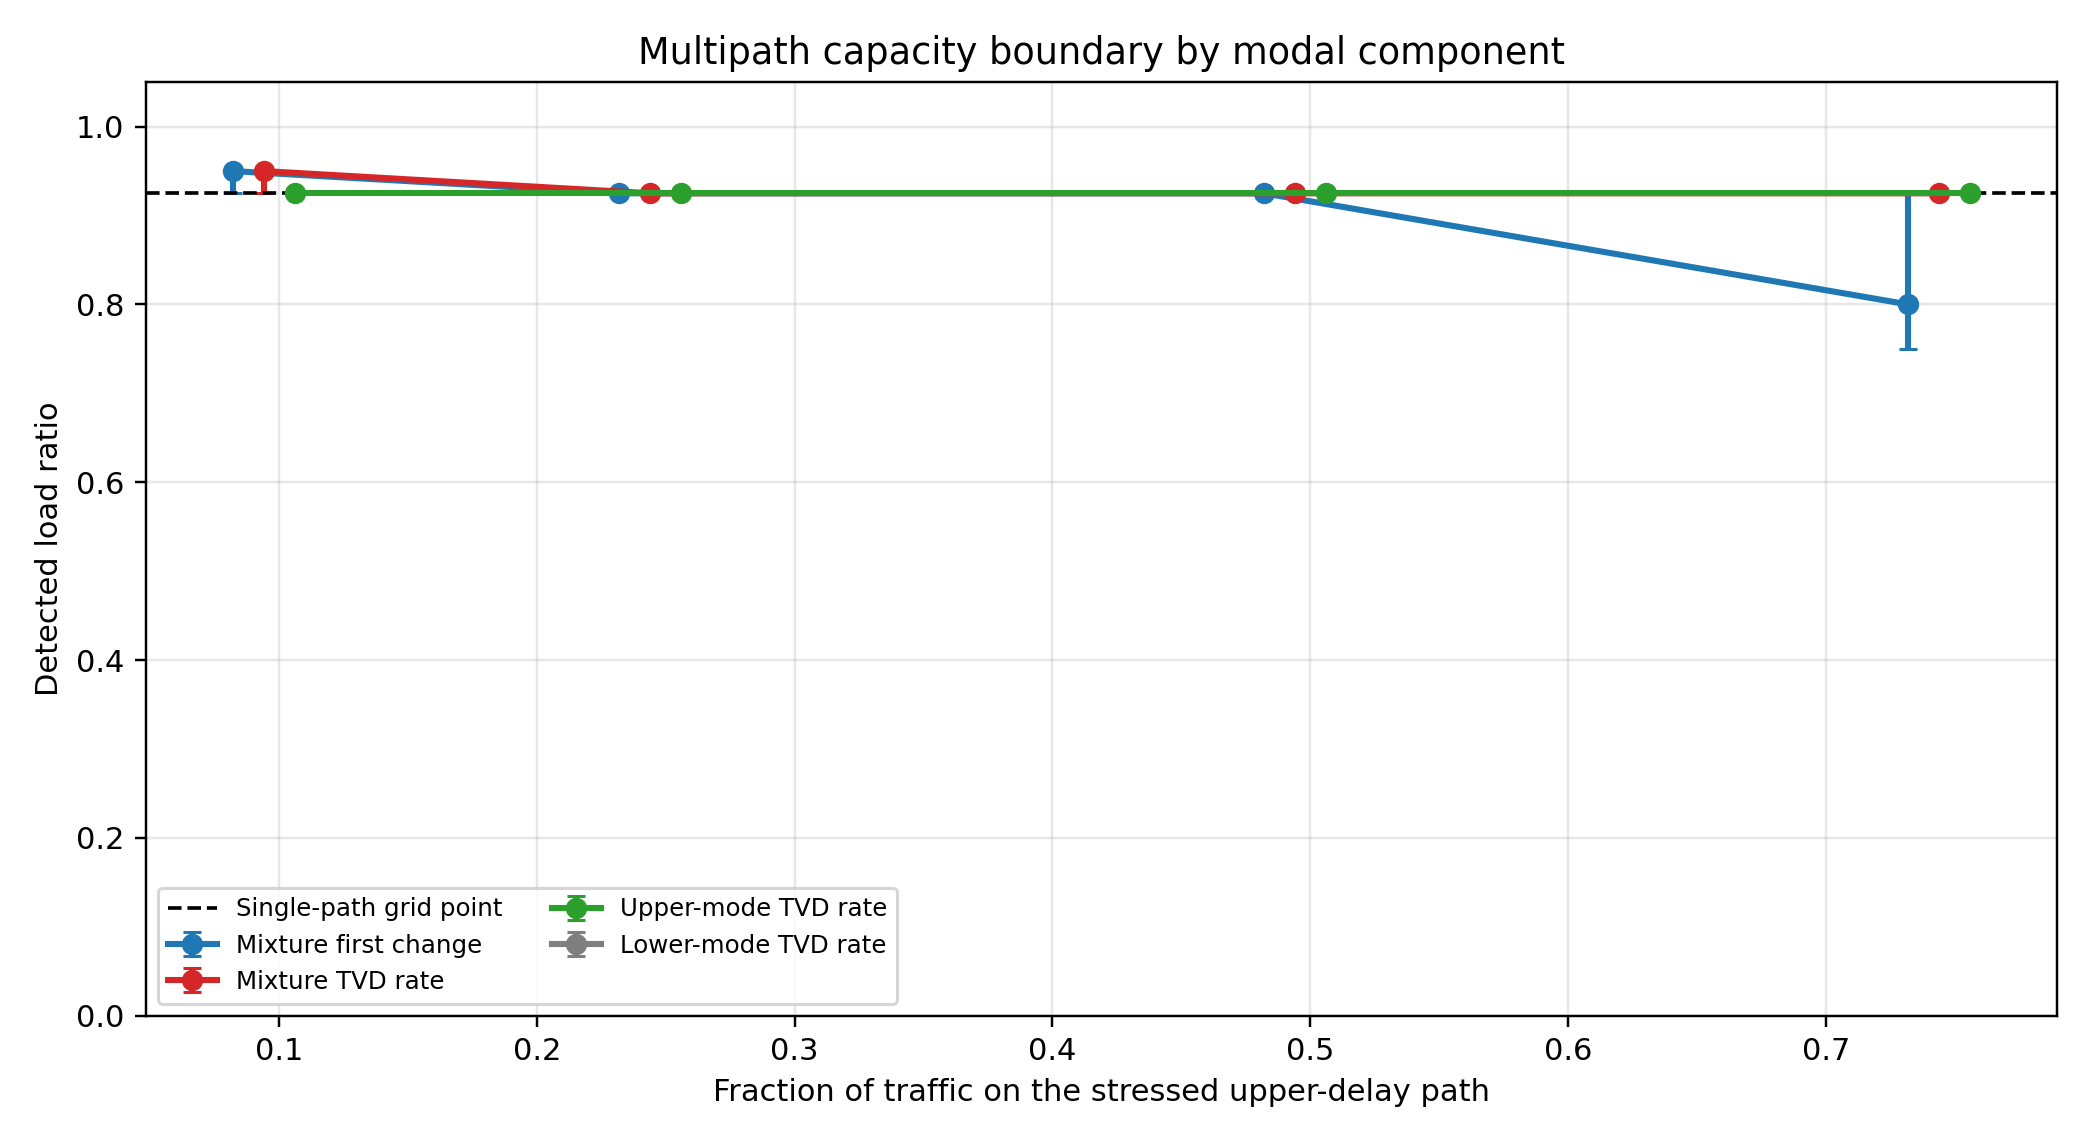
\includegraphics[width=\textwidth]{multipath_detection_by_method.png}
\caption{Detected capacity boundary in the multi-path mixture experiment. Whole-mixture rules depend on traffic share, while the upper-mode response remains aligned with the single-path grid point.}
\label{fig:multipath-methods}
\end{figure}

\begin{thebibliography}{99}

\bibitem{alFaresFatTree}
Mohammad Al-Fares, Alexander Loukissas, and Amin Vahdat.
\newblock A scalable, commodity data center network architecture.
\newblock In Proceedings of the ACM SIGCOMM Conference, pages 63 to 74, 2008.
\newblock \url{https://doi.org/10.1145/1402958.1402967}.

\bibitem{alFaresHedera}
Mohammad Al-Fares, Sivasankar Radhakrishnan, Barath Raghavan, Nelson Huang, and Amin Vahdat.
\newblock Hedera: Dynamic flow scheduling for data center networks.
\newblock In Proceedings of the USENIX Symposium on Networked Systems Design and Implementation, pages 281 to 296, 2010.
\newblock \url{https://www.usenix.org/conference/nsdi10/hedera-dynamic-flow-scheduling-data-center-networks}.

\bibitem{alizadehConga}
Mohammad Alizadeh, Tom Edsall, Sarang Dharmapurikar, Ramanan Vaidyanathan, Kevin Chu, Andy Fingerhut, Vinh The Lam, Francis Matus, Rong Pan, Navindra Yadav, and George Varghese.
\newblock CONGA: Distributed congestion-aware load balancing for datacenters.
\newblock In Proceedings of the ACM SIGCOMM Conference, pages 503 to 514, 2014.
\newblock \url{https://doi.org/10.1145/2619239.2626316}.

\bibitem{alizadehDctcp}
Mohammad Alizadeh, Albert Greenberg, David A. Maltz, Jitendra Padhye, Parveen Patel, Balaji Prabhakar, Sudipta Sengupta, and Murari Sridharan.
\newblock Data Center TCP (DCTCP).
\newblock In Proceedings of the ACM SIGCOMM Conference, pages 63 to 74, 2010.
\newblock \url{https://doi.org/10.1145/1851182.1851192}.

\bibitem{arfeenWeibull}
Asad Arfeen, Krzysztof Pawlikowski, Don McNickle, and Andreas Willig.
\newblock The role of the Weibull distribution in modelling traffic in Internet access and backbone core networks.
\newblock Journal of Network and Computer Applications, volume 141, pages 1 to 22, 2019.
\newblock \url{https://doi.org/10.1016/j.jnca.2019.05.002}.

\bibitem{barfordSignalAnalysis}
Paul Barford, Jeffery Kline, David Plonka, and Amos Ron.
\newblock A signal analysis of network traffic anomalies.
\newblock In Proceedings of the ACM SIGCOMM Internet Measurement Workshop, pages 71 to 82, 2002.
\newblock \url{https://doi.org/10.1145/637201.637210}.

\bibitem{chenConQuest}
Xiaoqi Chen, Shir Landau Feibish, Yaron Koral, Jennifer Rexford, Ori Rottenstreich, Steven A. Monetti, and Tzuu-Yi Wang.
\newblock Fine-grained queue measurement in the data plane.
\newblock In Proceedings of the ACM International Conference on emerging Networking EXperiments and Technologies, pages 15 to 29, 2019.
\newblock \url{https://doi.org/10.1145/3359989.3365408}.

\bibitem{benBasatPint}
Ran Ben Basat, Sivaramakrishnan Ramanathan, Yuliang Li, Gianni Antichi, Minlan Yu, and Michael Mitzenmacher.
\newblock PINT: Probabilistic in-band network telemetry.
\newblock In Proceedings of the ACM SIGCOMM Conference, pages 662 to 680, 2020.
\newblock \url{https://doi.org/10.1145/3387514.3405894}.

\bibitem{brutlagAberrant}
Jake D. Brutlag.
\newblock Aberrant behavior detection in time series for network monitoring.
\newblock In Proceedings of the 14th USENIX Conference on System Administration, pages 139 to 146, 2000.
\newblock \url{https://www.usenix.org/publications/library/proceedings/lisa2000/brutlag.html}.

\bibitem{canonneShort}
Clement L. Canonne.
\newblock A short note on learning discrete distributions.
\newblock arXiv:2002.11457, 2020.
\newblock \url{https://arxiv.org/abs/2002.11457}.

\bibitem{canonneSurvey}
Clement L. Canonne.
\newblock A Survey on Distribution Testing: Your Data is Big. But is it Blue?
\newblock Theory of Computing Library, Graduate Surveys 9, 2020.
\newblock \url{https://theoryofcomputing.org/articles/gs009/}.

\bibitem{canonneTopics}
Clement L. Canonne.
\newblock Topics and Techniques in Distribution Testing: A Biased but Representative Sample.
\newblock Foundations and Trends in Communications and Information Theory, volume 19, number 6, pages 1032 to 1198, 2022.
\newblock \url{https://ccanonne.github.io/files/misc/main-survey-fnt.pdf}.

\bibitem{devroyeLugosi}
Luc Devroye and Gabor Lugosi.
\newblock Combinatorial Methods in Density Estimation.
\newblock Springer, 2001.

\bibitem{claiseNetflow}
Benoit Claise.
\newblock Cisco Systems NetFlow Services Export Version 9.
\newblock RFC 3954, 2004.
\newblock \url{https://www.rfc-editor.org/rfc/rfc3954}.

\bibitem{dingRdProbe}
Rui Ding, Xunpeng Liu, Shibo Yang, Qun Huang, Baoshu Xie, Ronghua Sun, Zhi Zhang, and Bolong Cui.
\newblock RD-Probe: Scalable monitoring with sufficient coverage in complex datacenter networks.
\newblock In Proceedings of the ACM SIGCOMM Conference, 2024.
\newblock \url{https://doi.org/10.1145/3651890.3672256}.

\bibitem{dovrolisPacketDispersion}
Constantinos Dovrolis, Parameswaran Ramanathan, and David Moore.
\newblock Packet-dispersion techniques and a capacity-estimation methodology.
\newblock IEEE/ACM Transactions on Networking, volume 12, number 6, pages 963 to 977, 2004.
\newblock \url{https://doi.org/10.1109/TNET.2004.838606}.

\bibitem{downeyLognormal}
Allen B. Downey.
\newblock Lognormal and Pareto distributions in the Internet.
\newblock Computer Communications, volume 28, number 7, pages 790 to 801, 2005.
\newblock \url{https://doi.org/10.1016/j.comcom.2004.11.001}.

\bibitem{guoPingmesh}
Chuanxiong Guo, Lihua Yuan, Dong Xiang, Yingnong Dang, Ray Huang, Dave Maltz, Zhaoyi Liu, Vin Wang, Bin Pang, Hua Chen, Zhi-Wei Lin, and Varugis Kurien.
\newblock Pingmesh: A large-scale system for data center network latency measurement and analysis.
\newblock In Proceedings of the ACM SIGCOMM Conference, pages 139 to 152, 2015.
\newblock \url{https://doi.org/10.1145/2785956.2787496}.

\bibitem{greenbergVl2}
Albert Greenberg, James R. Hamilton, Navendu Jain, Srikanth Kandula, Changhoon Kim, Parantap Lahiri, David A. Maltz, Parveen Patel, and Sudipta Sengupta.
\newblock VL2: A scalable and flexible data center network.
\newblock In Proceedings of the ACM SIGCOMM Conference, pages 51 to 62, 2009.
\newblock \url{https://doi.org/10.1145/1592568.1592576}.

\bibitem{ghorbaniDrill}
Soudeh Ghorbani, Zibin Yang, P. Brighten Godfrey, Yashar Ganjali, and Amin Firoozshahian.
\newblock DRILL: Micro load balancing for low-latency data center networks.
\newblock In Proceedings of the ACM SIGCOMM Conference, pages 225 to 238, 2017.
\newblock \url{https://doi.org/10.1145/3098822.3098839}.

\bibitem{handigolNetSight}
Nikhil Handigol, Brandon Heller, Vimalkumar Jeyakumar, David Mazieres, and Nick McKeown.
\newblock I Know What Your Packet Did Last Hop: Using packet histories to troubleshoot networks.
\newblock In Proceedings of the USENIX Symposium on Networked Systems Design and Implementation, pages 71 to 85, 2014.
\newblock \url{https://www.usenix.org/conference/nsdi14/technical-sessions/presentation/handigol}.

\bibitem{hongSwan}
Chi-Yao Hong, Srikanth Kandula, Ratul Mahajan, Ming Zhang, Vijay Gill, Mohan Nanduri, and Roger Wattenhofer.
\newblock Achieving high utilization with software-driven WAN.
\newblock In Proceedings of the ACM SIGCOMM Conference, pages 15 to 26, 2013.
\newblock \url{https://doi.org/10.1145/2486001.2486012}.

\bibitem{harringtonSnmp}
David Harrington, Randy Presuhn, and Bert Wijnen.
\newblock An Architecture for Describing Simple Network Management Protocol (SNMP) Management Frameworks.
\newblock RFC 3411, 2002.
\newblock \url{https://doi.org/10.17487/RFC3411}.

\bibitem{hartiganDip}
John A. Hartigan and Pamela M. Hartigan.
\newblock The dip test of unimodality.
\newblock The Annals of Statistics, volume 13, number 1, pages 70 to 84, 1985.
\newblock \url{https://doi.org/10.1214/aos/1176346577}.

\bibitem{jainDovrolisPathload}
Manish Jain and Constantinos Dovrolis.
\newblock End-to-end available bandwidth: measurement methodology, dynamics, and relation with TCP throughput.
\newblock IEEE/ACM Transactions on Networking, volume 11, number 4, pages 537 to 549, 2003.
\newblock \url{https://doi.org/10.1109/TNET.2003.815304}.

\bibitem{jainB4}
Sushant Jain, Alok Kumar, Subhasree Mandal, Joon Ong, Leon Poutievski, Arjun Singh, Subbaiah Venkata, Jim Wanderer, Junlan Zhou, Min Zhu, Jonathan Zolla, Urs Holzle, Stephen Stuart, and Amin Vahdat.
\newblock B4: Experience with a globally-deployed software defined WAN.
\newblock In Proceedings of the ACM SIGCOMM Conference, pages 3 to 14, 2013.
\newblock \url{https://doi.org/10.1145/2486001.2486019}.

\bibitem{karakasDelay}
Mehmet Karakas.
\newblock Determination of network delay distribution over the internet.
\newblock M.S. thesis, Middle East Technical University, 2003.
\newblock \url{https://hdl.handle.net/11511/13840}.

\bibitem{lakhinaDistributions}
Anukool Lakhina, Mark Crovella, and Christophe Diot.
\newblock Mining anomalies using traffic feature distributions.
\newblock In Proceedings of the ACM SIGCOMM Conference, pages 217 to 228, 2005.
\newblock \url{https://doi.org/10.1145/1080091.1080118}.

\bibitem{lakhinaDiagnosing}
Anukool Lakhina, Mark Crovella, and Christophe Diot.
\newblock Diagnosing network-wide traffic anomalies.
\newblock In Proceedings of the ACM SIGCOMM Conference, pages 219 to 230, 2004.
\newblock \url{https://doi.org/10.1145/1015467.1015492}.

\bibitem{laiSequential}
Tze Leung Lai.
\newblock Sequential analysis: Some classical problems and new challenges.
\newblock Statistica Sinica, volume 11, number 2, pages 303 to 408, 2001.
\newblock \url{https://www3.stat.sinica.edu.tw/statistica/j11n2/j11n21/j11n21.htm}.

\bibitem{linLmsa}
Yu Lin, Shiduan Cheng, Chonggang Wang, Haitao Wu, Keping Long, and Shihong Zou.
\newblock A new approach for path capacity measurement in Internet.
\newblock High Speed Networks, volume 13, number 3, pages 183 to 206, 2004.
\newblock \url{https://doi.org/10.3233/HSN-2004-243}.

\bibitem{liuUnivMon}
Zaoxing Liu, Antonis Manousis, Gregory Vorsanger, Vyas Sekar, and Vladimir Braverman.
\newblock One sketch to rule them all: Rethinking network flow monitoring with UnivMon.
\newblock In Proceedings of the ACM SIGCOMM Conference, pages 101 to 114, 2016.
\newblock \url{https://doi.org/10.1145/2934872.2934906}.

\bibitem{moshrefTrumpet}
Masoud Moshref, Minlan Yu, Ramesh Govindan, and Amin Vahdat.
\newblock Trumpet: Timely and precise triggers in data centers.
\newblock In Proceedings of the ACM SIGCOMM Conference, pages 129 to 143, 2016.
\newblock \url{https://doi.org/10.1145/2934872.2934879}.

\bibitem{narayanaMarple}
Srinivas Narayana, Anirudh Sivaraman, Vikram Nathan, Prateesh Goyal, Venkat Arun, Mohammad Alizadeh, Vimalkumar Jeyakumar, and Changhoon Kim.
\newblock Language-directed hardware design for network performance monitoring.
\newblock In Proceedings of the ACM SIGCOMM Conference, pages 85 to 98, 2017.
\newblock \url{https://doi.org/10.1145/3098822.3098829}.

\bibitem{nychisEntropy}
George Nychis, Vyas Sekar, David G. Andersen, Hyong Kim, and Hui Zhang.
\newblock An empirical evaluation of entropy-based traffic anomaly detection.
\newblock In Proceedings of the ACM Internet Measurement Conference, pages 151 to 156, 2008.
\newblock \url{https://doi.org/10.1145/1452520.1452539}.

\bibitem{p4IntSpec}
P4 Applications Working Group.
\newblock In-band Network Telemetry (INT) Dataplane Specification, version 2.1.
\newblock 2020.
\newblock \url{https://p4.org/p4-spec/docs/INT_v2_1.pdf}.

\bibitem{pageCusum}
E. S. Page.
\newblock Continuous inspection schemes.
\newblock Biometrika, volume 41, number 1, pages 100 to 115, 1954.
\newblock \url{https://doi.org/10.1093/biomet/41.1-2.100}.

\bibitem{panMultipathDelay}
Sheng Pan, Yong Wang, Min Xiong, Li Gu, and Guo Min Hu.
\newblock Detection of multipath routing with passive delay measurements.
\newblock In Proceedings of the IEEE Conference on Computer Communications Workshops, pages 127 to 132, 2019.
\newblock \url{https://doi.org/10.1109/INFCOMW.2019.8845038}.

\bibitem{phaalSflow}
Peter Phaal, Sonia Panchen, and Neil McKee.
\newblock InMon Corporation's sFlow: A Method for Monitoring Traffic in Switched and Routed Networks.
\newblock RFC 3176, 2001.
\newblock \url{https://doi.org/10.17487/RFC3176}.

\bibitem{qiuPacketDoppler}
Tongqing Qiu, N. Hua, Jian Ni, Y. Richard Yang, and Hong Wang.
\newblock Packet Doppler: network monitoring using packet shift detection.
\newblock In Proceedings of the ACM CoNEXT Conference, pages 1 to 12, 2008.
\newblock \url{https://doi.org/10.1145/1544012.1544015}.

\bibitem{qureshiFathom}
Mubashir Adnan Qureshi, Junhua Yan, Yuchung Cheng, Soheil Hassas Yeganeh, Neal Cardwell, Yousuk Seung, Willem de Bruijn, Van Jacobson, Amin Vahdat, and David Wetherall.
\newblock Fathom: Understanding datacenter application network performance.
\newblock In Proceedings of the ACM SIGCOMM Conference, 2023.
\newblock \url{https://doi.org/10.1145/3603269.3604815}.

\bibitem{ribeiroPathchirp}
Vinay J. Ribeiro, Rudolf H. Riedi, Jiri Navratil, Les Cottrell, and Richard G. Baraniuk.
\newblock pathChirp: Efficient available bandwidth estimation for network paths.
\newblock SLAC Technical Report SLAC-PUB-9732, 2003.
\newblock \url{https://doi.org/10.2172/813038}.

\bibitem{shobhanaPirate}
Bhavana Vannarth Shobhana, Yen-lin Chien, Jonathan Diamant, Badri Nath, Shir Landau Feibish, and Srinivas Narayana.
\newblock Measuring round-trip response latencies under asymmetric routing.
\newblock arXiv:2505.14358, 2025.
\newblock \url{https://arxiv.org/abs/2505.14358}.

\bibitem{singhJupiter}
Arjun Singh, Joon Ong, Amit Agarwal, Glen Anderson, Ashby Armistead, Roy Bannon, Seb Boving, Gaurav Desai, Bob Felderman, Paulie Germano, Anand Kanagala, Hong Liu, Jeff Provost, Jason Simmons, Eiichi Tanda, Jim Wanderer, Urs Holzle, Stephen Stuart, and Amin Vahdat.
\newblock Jupiter Rising: A decade of Clos topologies and centralized control in Google's datacenter network.
\newblock ACM SIGCOMM Computer Communication Review, volume 45, number 4, pages 183 to 197, 2015.
\newblock \url{https://doi.org/10.1145/2829988.2787508}.

\bibitem{silvermanModes}
Bernard W. Silverman.
\newblock Using kernel density estimates to investigate multimodality.
\newblock Journal of the Royal Statistical Society: Series B, volume 43, number 1, pages 97 to 99, 1981.
\newblock \url{https://doi.org/10.1111/j.2517-6161.1981.tb01155.x}.

\bibitem{sommersSla}
Joel Sommers, Paul Barford, Nick Duffield, and Amos Ron.
\newblock Accurate and efficient SLA compliance monitoring.
\newblock In Proceedings of the ACM SIGCOMM Conference, pages 109 to 120, 2007.
\newblock \url{https://doi.org/10.1145/1282427.1282394}.

\bibitem{straussSpruce}
Jacob Strauss, Dina Katabi, and Frans Kaashoek.
\newblock A measurement study of available bandwidth estimation tools.
\newblock In Proceedings of the ACM SIGCOMM Internet Measurement Conference, pages 39 to 44, 2003.
\newblock \url{https://doi.org/10.1145/948205.948211}.

\bibitem{tsangDelayTomography}
Yolanda Tsang, Mark Coates, and Robert D. Nowak.
\newblock Network delay tomography.
\newblock IEEE Transactions on Signal Processing, volume 51, number 8, pages 2125 to 2136, 2003.
\newblock \url{https://doi.org/10.1109/TSP.2003.814520}.

\bibitem{waldSequential}
Abraham Wald.
\newblock Sequential tests of statistical hypotheses.
\newblock The Annals of Mathematical Statistics, volume 16, number 2, pages 117 to 186, 1945.
\newblock \url{https://doi.org/10.1214/aoms/1177731118}.

\bibitem{zhengMuMon}
Hao Zheng, Chengyuan Huang, Xiangyu Han, Jiaqi Zheng, Xiaoliang Wang, Chen Tian, Wanchun Dou, and Guihai Chen.
\newblock \(\mu\)Mon: Empowering microsecond-level network monitoring with wavelets.
\newblock In Proceedings of the ACM SIGCOMM Conference, pages 274 to 290, 2024.
\newblock \url{https://doi.org/10.1145/3651890.3672236}.

\bibitem{zhuEverflow}
Yibo Zhu, Nanxi Kang, Jiaxin Cao, Albert Greenberg, Guohan Lu, Ratul Mahajan, Dave Maltz, Lihua Yuan, Ming Zhang, Ben Y. Zhao, and Haitao Zheng.
\newblock Packet-level telemetry in large datacenter networks.
\newblock In Proceedings of the ACM SIGCOMM Conference, pages 479 to 491, 2015.
\newblock \url{https://doi.org/10.1145/2785956.2787483}.

\end{thebibliography}

\end{document}
